%\documentclass[a4paper, 12pt, oneside]{amsbook}
\documentclass[a4paper,oneside,12pt]{book}
\usepackage{setspace}
\usepackage{float}

%% PROFUNDIDADE DO SUMARIO %%%%
\setcounter{tocdepth}{2}

%%%% MISC %%%%%
\usepackage[useregional]{datetime2}

%%%%%%%%% TABELAS %%%%%%%%%
\usepackage[table]{xcolor}
%\usepackage{tablestyles}
\usepackage{tabularx}
\usepackage{booktabs}
\usepackage{multirow}
\usepackage{xcolor}
%%%%%%%%%%%%%%%%%%%%%%%%%%%

%%%%%%%%%%%%%%%%%%%%%%%%%%%%%%%

%%%%%% MARGENS %%%%%%
%\usepackage{anysize}
\sloppy
%\setstretch{1.125}
\usepackage{geometry}
%\usepackage[headheight=16pt, vmargin=1in,hmargin=1in]{geometry}
%\stretch{1}
\usepackage{marginnote}
\usepackage[bottom]{footmisc}

%%%%%%%%%%%%%%%%%%%%%%%%%%%%%%

%%%%%% FONTES %%%%%%%%%
%\usepackage[light,math]{anttor}
\usepackage[T1]{fontenc}

%\renewcommand*\familydefault{\sfdefault} %%
%\usepackage{sfmath}
%\usepackage[usenames,dvipsnames]{xcolor}

%\usepackage{tgbonum} %% <---- Fonte teen ("How do you do fellow kids?")
%\usepackage{tgschola}
%\usepackage{helvet}
%\fontfamily{qcr}\selectfont
%\usepackage{lmodern}

%%%%%%%%%%%%%%%%%%%%%%

%%%%%%% CONTADORES %%%%%
\makeatletter
\def\providecounter#1{%
  \@ifundefined{c@#1}%
    {\newcounter{#1}}{\@newctr}}
\makeatother

\usepackage{enumitem}% http://ctan.org/pkg/enumitem
%%%%%%%%%%%%%%%%%%%%%%

%%%%%% links %%%%%%%%%%
\usepackage{hyperref}
\usepackage{url}
\hypersetup{
    colorlinks=true,
    linkcolor=blue,
    % filecolor=magenta,      
    % urlcolor=cyan,
    % pdftitle={Overleaf Example},
    % pdfpagemode=FullScreen,
    }
%%%%%%%%%%%%%%%%%%%%%%%

%%%%%%% Português %%%%%%%%
\usepackage[utf8]{inputenc}
\usepackage[brazil]{babel}
%%%%%%%%%%%%%%%%%%%%%%%%%

%%%%%%% Condicionais %%%%%%%
\usepackage{xifthen}
%%%%%%%%%%%%%%%%%%%%%%%%%%%

%%%%%%% Figuras e Tikz %%%%%%%
\usepackage{incgraph}
\usepackage{tikz}

% \usetikzlibrary{external}
% \tikzexternalize % activate!

\usepackage{graphicx}
\usetikzlibrary{shapes.geometric, arrows, arrows.meta} % diamonds e outras formas
\usetikzlibrary{decorations.pathreplacing}
\usetikzlibrary{decorations.pathmorphing}
\usetikzlibrary{bending}
\usetikzlibrary{positioning}
\usetikzlibrary{tikzmark}
\usetikzlibrary{calc}
\usetikzlibrary{patterns}
\usetikzlibrary{fadings}
% \usetikzlibrary{patterns.meta}

\usepackage{dot2texi}

\usepackage{framed}
\usepackage{caption}
\usepackage{subcaption}
%\usepackage{subfig}
%%%%%%%%%%%%%%%%%%%%%%%%%%%


%%%%%% Matemática %%%%%%%
\usepackage{amsmath, amssymb}
\usepackage{amsthm} %% teoremas
\newtheorem{theorem}{Teorema}
\newtheorem{prop}{Proposição}
%%%%%%%%%%%%%%%%%%%%%%%%%%

%%%%% ALGORITMOS %%%%%%%
\usepackage{mathtools}
\usepackage[ruled, vlined, linesnumbered, portuguese,onelanguage]{algorithm2e}
%%%%%%%%%%%%%%%%%%%%%%

%%%%%%%% CÓDIGO %%%%%%%%
\usepackage{listings}
\renewcommand{\lstlistingname}{Código}
\usepackage[scaled=0.9]{DejaVuSansMono}
\lstdefinestyle{cplusplusListStyle}{
  % backgroundcolor=\color{blue!10},
  belowcaptionskip=1\baselineskip,
  breaklines=true,
  xleftmargin=\parindent,
  language=C++,
  % frame=lrtb,
  frame=tb,
  showstringspaces=false,
  tabsize=2,
  %basicstyle=\footnotesize,
  basicstyle=\footnotesize\ttfamily,
  keywordstyle=\bfseries\color{green!40!black},
  commentstyle=\itshape\color{purple!40!black},
  identifierstyle=\color{blue},
  stringstyle=\color{orange},
numbers=left,
stepnumber=1
}
%%%%%%%%%%%%%%%%%%%%%%

%%%% headers %%%%% %%%%%
\usepackage[fit]{truncate}
\usepackage{fancyhdr}
\pagestyle{headings}
\pagestyle{fancy}
\fancyhf{}
\fancyfoot{}
%\rhead{\rightmark}
%\lhead{\truncate{.5\headwidth}{\leftmark}}
\chead{\leftmark}
% \rhead{\thepage}
\renewcommand{\headrulewidth}{0pt}
%\lhead{\leftmark}
\cfoot{\thepage}
%%%%%%%%%%%%%%%%%%%%%%%%

%%%%%%%%%%% CHAPTER STYLE %%%%%%%%%%%
\usepackage{titlesec}
\titleformat{\chapter}[display]
  {\normalfont\bfseries\centering}{\Huge\textbf{\fontsize{70}{80}\selectfont\thechapter}\vspace{0.25cm}}{0pt}{\LARGE}
%%%%%%%%%%%%%%%%%%%%%%%%

%%%%%%%%% COMANDOS %%%%%%%%%%% 
\renewcommand{\chaptermark}[1]{\markboth{\textit{#1}}{}}
\newcommand{\referencia}{{\color{blue} REF}}
%%%%%%%%%%%%%%%%%%%%%%%%

\title{O Kit}
%\author{}
%\date{2020}

\begin{document}

% % CAPA %
% \begin{center}
% %\vspace*{2cm}
% \Large \textbf{OTIMIZAÇÃO COMBINATÓRIA} \\ 
% \vspace{0.5cm}
% \vspace{0.75cm}
% \vspace{0.5cm}
% 
% \end{center}
% \vspace{2cm}
% 
% \begin{figure}[H]
% \centering
% 
% 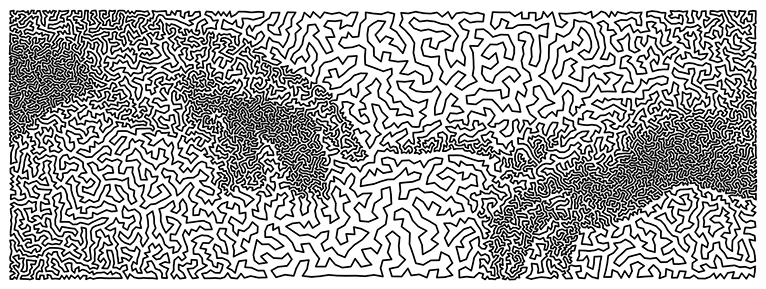
\includegraphics[width=1\textwidth]{imagens/tsp_art.jpg}
% \end{figure}
% \vspace*{\fill}
% \begin{center}
% 
% %\textbf{LASER-GO} \\
% \textbf{UFPB}
% \end{center}

\incgraph[documentpaper,
  overlay={\node[red] at (page.center) {};}]
  [width=\paperwidth,height=\paperheight]{capa.jpg}

%\maketitle
% \thispagestyle{empty}

\tableofcontents

%\part{Meta-heurísticas}

% \newpage
% \thispagestyle{empty}

\chapter*{Prefácio}
\thispagestyle{empty}
Compilado em \today.
% tem que ver 


\part{Heurísticas Gulosas e Busca Local}
\thispagestyle{empty}

\chapter{Introdução}
Um problema é dito de otimização combinatória quando envolve escolher uma solução ótima de um conjunto finito de soluções. Neste capítulo serão abordados conceitos importantes sobre grafos, que são importantes na otimização combinatória.

\section{Grafos}
Sejam $V$ e $E$ conjuntos de nós e arestas, respectivamente, o par \(G = (V, E)\) é considerado um grafo. Mais precisamente, \(E\) é um conjunto de pares \(\{i, j\}\) tais que \(i, j \in V, i \neq j\). Em outras palavras, qualquer conjunto de nós e arestas que conectem esses nós pode ser considerado um grafo. Um exemplo de grafo é mostrado na Figura \ref{fig:exemploGrafo}. Nela, \(V = \{1,2,3,4,5\}\) e \(E = \{\{1,2\}, \{2,3\}, \{2,4\}, \{3,5\}\}\).

\begin{figure}[!htbp]
    \centering
    \tikzset{mystyle/.style={circle, draw=black,inner sep=0pt, minimum width=12pt}}

    \begin{tikzpicture}
    
    \node[mystyle] (v1) at (-3,0) {1};
    \node[mystyle] (v2) at (0,2.5) {2};
    \node[mystyle] (v3) at (1,-2.5) {3};
    \node[mystyle] (v4) at (3,2) {4};
    \node[mystyle] (v5) at (4,-0.5) {5};
    \draw[-] (v1)--(v2);
    \draw[-] (v2)--(v3);
    \draw[-] (v5)--(v3);
    \draw[-] (v2)--(v4);

    
    \end{tikzpicture} 
    \caption{Exemplo de grafo não-orientado.}
    \label{fig:exemploGrafo}
\end{figure}

\subsection{Grafo completo}
Se, num grafo \(G = (V, E)\), a condição \(\{i, j\} \in E \;\; \forall i,j \in V, i \neq j\) é satisfeita (todos os nós estão conectados uns aos outros por arestas), \(G\) é um grafo completo.

\subsection{Grafo orientado}
Se, num grafo \(G = (V, E)\), \(\{i, j\} \neq \{j, i\} \;\; \forall i, j \in V, i \neq j\), \(G\) é um grafo orientado (ou dirigido), e \((i, j), (j, i) \in E\) são considerados arcos (e não arestas). Um exemplo de grafo orientado é mostrado na Figura \ref{fig:exemploGrafoOrientado}.

\subsection{Caminho}
Considere um grafo \(G = (V, E)\). Se houver uma sequência de nós \((v_1, \dots, v_n)\), a sequência de arestas \(e_i = \{v_i, v_{i+1}\} \in E, 1 \leq  i \leq n-1\) é um caminho. Observe que tanto a sequência de nós quanto a sequência de arestas podem possuir repetições.

\subsection{Ciclo}
Um ciclo é um caminho que inicia e termina em um nó.

\subsection{Ciclo Hamiltoniano}
Um ciclo Hamiltoniano é um ciclo que visita todos os nós de um grafo uma única vez.

\begin{figure}[!htbp]
    \centering
    \tikzset{mystyle/.style={circle, draw=black,inner sep=0pt, minimum width=12pt}}

    \begin{tikzpicture}
    
    \node[mystyle] (v1) at (-3,0) {1};
    \node[mystyle] (v2) at (0,2.5) {2};
    \node[mystyle] (v3) at (1,-2.5) {3};
    \node[mystyle] (v4) at (3,2) {4};
    \node[mystyle] (v5) at (4,-0.5) {5};
    \draw[->] (v1)--(v2);
    \draw[->] (v2)--(v3);
    \draw[->] (v5)--(v3);
    \draw[->] (v2)--(v4);
    \end{tikzpicture} 
    \caption{Exemplo de grafo orientado.}
    \label{fig:exemploGrafoOrientado}
\end{figure}

\section{TSP}
O Problema do Caixeiro Viajante (\textit{Traveling Salesman Problem} (TSP), em inglês) se trata de um problema de otimização combinatória famoso na literatura. Dado um grafo \(G = (V, E)\), em que \(V\) é um conjunto de cidades e \(c_{ij}\) é o custo de viagem da cidade \(i \in V\) para a cidade \(j \in V\) --- associado às arestas \(\{i, j\} \in E\) ---, o TSP visa  encontrar o ciclo Hamiltoniano (ou rota) que possui o custo de viagem total mínimo.

\subsection{Instâncias do TSP}
Qualquer conjunto de cidades com latitudes e longitudes --- ou coordenadas quaisquer --- pode ser entendido como uma instância do TSP. Em posse dessas coordenadas, é possível calcular a distância entre qualquer par de cidades. É possível, ainda, associar essas distâncias a uma matriz \(M\), na qual o elemento \(m_{ij}\) representa a distância entre a cidade \(i\) e a cidade \(j\).

Na Figura \ref{fig:instanciaTSP}, um grafo completo e não orientado com 4 nós representa uma instância do TSP. Os números próximos às arestas representam as distâncias entre as cidades. A mesma instância pode ser representada pela matriz de distâncias\footnote{Quando a instância se trata de um grafo não orientado --- como no exemplo ---, a matriz \(M\) é simétrica.} \[M = \begin{bmatrix}
0 & 40 & 30 & 20  \\
40 & 0 & 35 & 25  \\
30 & 35 & 0 & 45  \\
20 & 25 & 45 & 0  \\
\end{bmatrix}.\]

\begin{figure}[!htbp]
    \centering
    \tikzset{mystyle/.style={circle, draw=black,inner sep=0pt, minimum width=16pt}}

    \begin{tikzpicture}
    
    \node[mystyle] (v1) at (0,1) {1};
    \node[mystyle] (v2) at (0,5) {2};
    \node[mystyle] (v3) at (6,0) {3};
    \node[mystyle] (v4) at (4,7) {4};
   
   \path
    (v1) edge node [left] {40} (v2)
    (v1) edge node [below] {30} (v3)
    (v1) edge node [below right]{20} (v4)
    
    (v2) edge node [below left] {35} (v3)
    (v2) edge node [above] {25} (v4)

    (v3) edge node [right] {45} (v4);


    
    \end{tikzpicture} 
    \caption{Exemplo de instância.}
    \label{fig:instanciaTSP}
\end{figure}

\section{Meta-heurísticas e algoritmos exatos}
Os métodos heurísticos visam obter boas soluções para problemas de otimização combinatória em pouco tempo. Contudo, soluções ótimas não são garantidas. As meta-heurísticas são procedimentos genéricos que fazem uso de métodos heurísticos para resolver problemas de otimização. Uma mesma meta-heurística pode ser adaptada para resolver diferentes problemas --- levando-se em conta as particularidades de cada um. 

Os algoritmos exatos, por sua vez, garantem a obtenção de soluções ótimas --- embora não consigam fazê-lo em pouco tempo, muitas vezes.

Tanto as meta-heurísticas quanto os algoritmos exatos serão abordados nos próximos capítulos.

\chapter{Abordagem meta-heurística para o TSP}
\thispagestyle{empty}

Uma meta-heurística é um método heurístico para resolver problemas de otimização combinatória de forma genérica. Uma única meta-heurística pode ser reutilizada para resolver vários problemas diferentes, exigindo, por vezes, pouco esforço de adaptação para cada um deles. Este capítulo descreve a meta-heurística \textit{Iterated Local Search} (ILS), além das devidas adaptações necessárias para utilizá-la para resolver o TSP.

\section{\textit{Framework} ILS}
Considere um problema de otimização combinatória qualquer. Assuma que o problema é de minimização. O código a seguir apresenta um algoritmo genérico para resolvê-lo: 

%\begin{lstlisting}[style=cplusplusListStyle, caption={Framework do ILS.}, label={lst:ilsAlg}]
\begin{lstlisting}[style=cplusplusListStyle]
Solution ILS(int maxIter, int maxIterIls)
{
	Solution bestOfAll;
	bestOfAll.cost = INFINITY;
	for(int i = 0; i < maxIter; i++)
	{
		Solution s = Construcao();
		Solution best = s;
	
		int iterIls = 0;
	
		while(iterIls <= maxIterIls)
		{
			BuscaLocal(&s);
			if(s.cost < best.cost)
			{
				best = s;
				iterIls = 0;		
			}
			s = Perturbacao(best);
			iterIls++;
		}
		if (best.cost < bestOfAll.cost)
			bestOfAll = best;	
	}

return bestOfAll;
}
\end{lstlisting}

Primeiramente, algoritmo constrói uma solução baseando-se em palpites educados através do método Construção() (linha 7). Em seguida, tenta-se melhorar o custo dessa solução fazendo-se pequenas modificações através do método BuscaLocal() enquanto houver melhoras (linhas 14--18). Quando não for mais possível melhorar a solução, continua-se a partir de uma cópia levemente modificada da melhor solução da iteração corrente \texttt{best}, gerada pelo procedimento Perturbação() (linha 20). Continua-se até que um critério de parada seja atingido (linha 12). Se \texttt{best.cost} for menor que \texttt{bestOfAll.cost}, \texttt{best} passa a ser a melhor solução (linhas 23 e 24). Esse processo é repetido \texttt{maxIter} vezes (linha 5), e a melhor solução \texttt{bestOfAll} é retornada (linha 27).

Os procedimentos Construção(), BuscaLocal() e Perturbação() serão explicados em detalhes para o caso do TSP nas próximas seções. Recomenda-se que o leitor implemente-os na ordem em que são apresentados, para que então possa implementar o código acima.

\iffalse

O algoritmo possui três rotinas principais: (i) construir uma solução para a instância do problema baseando-se em palpites educados (método Construção()); (ii) buscar soluções parecidas com a solução corrente de forma a diminuir o seu valor objetivo através de pequenas modificações (método BuscaLocal()); e (iii) quando não for mais possível encontrar melhorias durante a busca local, modificar levemente a solução de forma aleatória (método Perturbação()).

\begin{figure}
    \begin{center}
    \scalebox{0.9}{
\begin{tikzpicture}[node distance=2cm, cross/.style={path picture={ 
  \draw[black]
(path picture bounding box.south east) -- (path picture bounding box.north west) (path picture bounding box.south west) -- (path picture bounding box.north east);
}}]
\tikzstyle{startstop} = [rectangle, rounded corners, minimum width=3cm, minimum height=1cm,text centered, draw=black, fill=red!30]
\tikzstyle{io} = [trapezium, trapezium left angle=70, trapezium right angle=110, minimum width=3cm, minimum height=1cm, text centered, align=center, draw=black, fill=blue!30]
\tikzstyle{process} = [rectangle, minimum width=3cm, minimum height=1cm, text centered, align = center, draw=black, fill=orange!30]
\tikzstyle{decision} = [diamond,aspect=2, minimum width=3cm, minimum height=1cm, text centered, align = center, draw=black, fill=green!30]
\tikzstyle{arrow} = [thick,->,>=latex, rounded corners]


\node (construction) [process] { \(s \leftarrow \text{Construção}()\)\\ \(s' \leftarrow s\) \\ \(\texttt{iterILS} \leftarrow 0\) }; 

\node (startAlgorithm) [startstop, above of = construction, xshift = -5cm] {Início};
\node (algorithmInput) [io, above of = construction] {\(\texttt{i} \leftarrow 0\) \\ \(s^* \leftarrow \infty\)};

\node (assignS1) [process, below of = construction, yshift = -0.25cm] {\(s' \leftarrow s\) \\ \(\texttt{iterILS} \leftarrow 0\)}; 
\node (isItBetter) [decision, below of = assignS1, yshift = -0.7cm] {\(f(s) < f(s')\)};
\node (localSearch) [process, below of = isItBetter, yshift = -0.5cm] {\(s \leftarrow \text{BuscaLocal}(s)\)};


\node (perturbation) [process, right of = isItBetter, xshift = 3.5cm] {\(s \leftarrow \text{Perturbação}(s')\) \\ \(\texttt{iterILS} \leftarrow \texttt{iterILS} + 1\) };


\node (keepGoing) [decision, below of = localSearch, yshift = -1cm] {\(\texttt{iterILS} \leq \texttt{maxIterILS}\)};
\node (betterThanBestOfAll) [decision, below of = keepGoing, yshift = -1.5cm] {\(f(s') < f(s^*)\)};
\node (updateBestOfAll) [process, below of = betterThanBestOfAll, yshift = -1cm] {\(s^* \leftarrow s'\)};

\node (auxNode1) [circle,cross, draw=black, left of = betterThanBestOfAll, xshift=-1cm] {};
%\node (auxNode2) [circle,cross, draw=black, left of = construction, xshift=-1.5cm] {};


\node (restart) [decision, left of = auxNode1, xshift = -0.35cm] {\(\texttt{i} \leq \texttt{N}\)};

\node (stopAlgorithm) [startstop, below of = restart, yshift = -0.5cm] {Fim};
\node (updateRestart) [process, above of = restart, yshift=1cm] {\(\texttt{i} \leftarrow \texttt{i} + 1\)};

%\node (localSearch) [process, below of = construction] {Busca local};

%\draw [arrow] (isItBetter.west) -| ++(-1.5,0)  node[anchor=north] {Sim} |- (assignS1.west);

\draw [arrow] (isItBetter.north) --  node[anchor=east] {Sim}  (assignS1.south);
\draw [arrow] (assignS1.east) -| (perturbation.north);
\draw [arrow] (localSearch.north) -- (isItBetter.south);
\draw [arrow] (isItBetter.east) -- node[anchor=north] {Não} (perturbation.west);
\draw [arrow] (perturbation.south) |- (keepGoing.east);
%\draw [arrow] (startIls) -- (construction);
%\draw [arrow] (construction.west)  -- ++(-1,0) |-  (localSearch.west);
\draw [arrow] (keepGoing.north) -- node[anchor=east]{Sim} (localSearch.south);
\draw [arrow] (keepGoing.south) -- node[anchor=east]{Não} (betterThanBestOfAll.north);

\coordinate (coord1) [above of = construction];

\draw[arrow] (betterThanBestOfAll.south) -- node[anchor=east]{Sim}  (updateBestOfAll.north);
\draw[arrow] (betterThanBestOfAll.west)--  node[anchor=south, yshift = 0.1cm]{Não}  (auxNode1.east);


\draw[arrow] (updateBestOfAll.west) -| (auxNode1.south);
\draw[arrow] (auxNode1.west) -- (restart.east);
\draw[arrow] (updateRestart.north) |- (construction.west);
\draw[arrow] (restart.south) -- node[anchor = east]{Não} (stopAlgorithm.north);
\draw[arrow] (restart.north) -- node[anchor = east]{Sim} (updateRestart.south);

\draw[arrow] (construction.south) |- ++(-3,-0.3) |- (localSearch);

\draw[arrow] (startAlgorithm) -- (algorithmInput.west);
\draw[arrow] (algorithmInput.south) -- (construction);

\end{tikzpicture}}
\end{center}
    \caption{Fluxograma da meta-heurística ILS.}
    \label{fig:ILSFlowChart}
\end{figure}
\fi

\section{Construção()}
Uma heurística construtiva busca criar uma solução razoável para um problema de otimização. A solução criada pode então ser modificada e melhorada ao longo do tempo. Por esse motivo, é comum que o valor objetivo de soluções geradas por procedimentos esteja longe do valor ótimo. A heurística construtitva  utilizada no método Construção() baseia-se no método \textit{Greedy Randomized Adaptive Search Procedure} (GRASP) \referencia{}. 

\subsection{Inserção mais barata}
Considere uma instância do TSP dada pelo grafo completo com pesos \(G = (V,E)\). Considere, ainda, um subconjunto arbitrário de vértices \(V' \subset V\), e que \(s'\) é um \textit{tour} que visita todos os vértices de \(V'\)\footnote{Nesse caso, diz-se que \(s'\) é um \textit{subtour}, já que visita apenas alguns vértices de \(V\).}. Seja \(CL = V \setminus V'\) uma lista de candidatos a serem inseridos em \(s'\) de forma a obter um \textit{tour} completo.

Analisemos o que ocorre quando um único vértice \(k \in CL\) é inserido em \(s'\). Note que para isso, é sempre necessário colocar \(k\) entre dois vértices adjacentes \(i\) e \(j\). Essa operação implica na remoção da aresta \(\{i,j\}\), e na adição de duas arestas \(\{i,k\}\) e \(\{k,j\}\). Suponha que \(s''\) é um novo \textit{subtour}, resultado da inserção de \(k\) em \(s'\). A partir disso, deduz-se que o custo de inserção de \(k\) em \(s'\) é \(\Delta = f(s'') - f(s') = c_{ik} + c_{kj} - c_{ij}\). Um exemplo dessa operação é mostrado na Figura \ref{fig:insercaoMaisBarata}, na qual o vértice 5 é inserido entre os vértices 1 e 3, resultando em um novo \textit{subtour}.


\begin{figure}[t]
    \centering
    \begin{tikzpicture}
    \tikzstyle{vertex} = [circle, rounded corners, minimum width=0.5cm, minimum height=0.625cm,text centered, draw=black, fill=white]
    
    \node[vertex] (v1) at  (-2,-2) {1};
    \node[vertex] (v4) at  (2,2) {4};
    \node[vertex] (v6) at  (-2,2) {6};
    \node[vertex] (v3) at  (2,-2) {3};
    \node[vertex] (v5) at (0, -4) {5};
    
    \draw[-] (v1)--(v6);
    \draw[-] (v6)--(v4);
    \draw[-] (v4)--(v3);
    \draw[-] (v1)--(v3);
    
        
    \node[vertex] (v11) at  (4,-2) {1};
    \node[vertex] (v41) at  (8,2) {4};
    \node[vertex] (v61) at  (4,2) {6};
    \node[vertex] (v31) at  (8,-2) {3};
    \node[vertex] (v5) at (6, -4) {5};
    
    \draw[->,>=stealth, ultra thick] (2.5,0) -- (3.5,0);
    
    \draw[-] (v11)--(v61);
    \draw[-] (v61)--(v41);
    \draw[-] (v41)--(v31);
    \draw[dashed, color = red, ultra thick] (v11)-- node[yshift = 0.5cm]{\(-c_{1,3}\)}(v31);
    
    \draw[-, color = blue, ultra thick] (v11)-- node[xshift = -0.5cm, yshift = -0.25cm]{\(+c_{1,5}\)}(v5);
    \draw[-, color = blue, ultra thick] (v31)--node[xshift = 0.5cm, yshift = -0.25cm]{\(+c_{5,3}\)}(v5);
    
    \end{tikzpicture} 
    \caption{Inserção de um novo nó.}
    \label{fig:insercaoMaisBarata}
\end{figure}

É fácil perceber que escolher o vértice \(k\) e a aresta \(\{i,j\}\) de forma a minimizar \(\Delta\) significa diminuir o prejuízo no valor objetivo após a inserção. No entanto, escolher sempre o par \((k, \{i,j\})\) que minimiza \(\Delta\) pode ``viciar'' o método, levando-o sempre a soluções parecidas, o que pode dificultar as buscas locais. Portanto, convém introduzir um pouco de aleatoriedade na escolha do par. Baseando-se nessas ideias, pode-se enumerar as etapas do método Construção() como segue.

\begin{enumerate}
    \item Construir uma solução parcial \(s'\) de forma aleatória; \label{insercaomaisbaratainicio}
    \item \(V' \leftarrow \) vértices de \(s'\) e \(CL \leftarrow V \setminus V'\); 
    \item Computar os pares \((k, \{i,j\})\) para todo \(k \in CL\), \(\{i,j\} \in s'\) e armazená-los em uma lista \(\Omega\); \label{insercaomaisbarataloop}
    \item Ordenar os pares em \(\Omega\) em ordem crescente de \(\Delta\);
    \item \(\alpha \leftarrow\) número aleatório no intervalo \([0,1]\);
    \item Selecionar aleatoriamente um dos \(\lfloor \alpha \times |\Omega| \rfloor \) primeiros pares em \(\Omega\);
    \item Sendo \((k, \{i,j\})\) o par escolhido, retirar a aresta \(\{i,j\}\) de \(s'\) e inserir o vértice \(k\) entre $i$ e $j$;
    \item Remover \(k\) da lista de candidatos \(CL\);
    \item Se \(CL\) estiver vazio, retornar \(s'\). Senão, voltar para o passo \ref{insercaomaisbarataloop}.
\end{enumerate}

É suficiente construir o \textit{subtour} inicial do passo \ref{insercaomaisbaratainicio} com 3 vértices. Para isso, pode-se iniciar \(s'\) sempre como \texttt{s' = \{1, 1\}} e inserir 3 vértices de forma aleatória. Assim, o \textit{subtour} inicial da  Figura \ref{fig:insercaoMaisBarata}, por exemplo, seria \texttt{s' = \{1,6,4,3,1\}}.

Um exemplo de implementação do procedimento Construção() pode ser visto a seguir:

%\begin{lstlisting}[style=cplusplusListStyle, caption={Procedimento Construção().}, label={lst:construction}]
\begin{lstlisting}[style=cplusplusListStyle]
struct InsertionInfo
{
	int noInserido; // no k a ser inserido
	int arestaRemovida; // aresta {i,j} na qual o no k sera inserido
	double custo; // delta ao inserir k na aresta {i,j}
};
    
std::vector<InsertionInfo> calcularCustoInsercao(Solution& s, std::vector<int>& CL)
{
	std::vector<InsertionInfo> custoInsercao = std::vector<InsertionInfo> custoInsercao((s.size() - 1) * CL.size());
	int l = 0;	
	for(int a = 0; a < s.sequence.size() - 1; a++) {
		int i = s.sequence[a];
		int j = s.sequence[a + 1];
		for (auto k : CL) {
			custoInsercao[l].custo = c[i][k] + c[j][k] - c[i][j];
			custoInsercao[l].noInserido = k;
			custoInsercao[l].arestaRemovida = a;
			l++;
		}
	}
	return custoInsercao;
}

Solution Construcao()
{
	Solution s;
	s.sequence = escolher3NosAleatorios();
	std::vector<int> CL = nosRestantes();
	/* Ex: V = {1,2,3,4,5,6,7,8,9,10}
		 s.sequence = {1,2,9,5,1} 
		 CL = {3,4,6,7,8,10} */
	while(!CL.empty()) {
		std::vector<InsertionInfo> custoInsercao = calcularCustoInsercao(s, CL);
		ordenarEmOrdemCrescente(custoInsercao);
		double alpha = (double) rand() / RAND_MAX;
		int selecionado = rand() % ((int) ceil(alpha * custoInsercao.size()));
		inserirNaSolucao(s, custoInsercao[selecionado].k);
	}

    return s;
}
\end{lstlisting}

No exemplo, armazena-se as informações de cada par \((k, \{i,j\})\) em uma estrutura do tipo \texttt{InsertionInfo}. Os custos de inserção de cada par \((k, \{i,j\})\) são calculados pela função \texttt{calcularCustoInsercao()}, que é chamada na função \texttt{Construcao()} até que $CL$ esteja vazio.


\section{BuscaLocal()}
A etapa de busca local possui como objetivo melhorar a solução corrente no decorrer da execução do algoritmo. O procedimento é feito modificando-se as soluções e avaliando o impacto das modificações na função objetivo. Antes de descrever o procedimento BuscaLocal(), alguns conceitos são apresentados nas subseções que seguem.

\subsection{Movimentos}
Seja \(s\) uma solução viável qualquer para um problema de otimização, e \(m\) uma operação que altera \(s\) de alguma maneira. Diz-se que \(m\) é um ``movimento'', e que \(s' =  s \oplus m \) é  uma nova solução, obtida após executá-lo. Há varios tipos de movimentos possíveis, que dependem, por sua vez, do problema de otimização em questão. Um exemplo de movimento para o TSP é trocar as posições de dois vértices na sequência.

\subsection{Estruturas de vizinhança}
Sejam \(s\) uma solução qualquer, e \(M_k\) um conjunto de movimentos estruturalmente parecidos. O conjunto \(\mathcal{N}_k (s)\) contém todas as posíveis soluções que se poderia obter executando em \(s\) os movimentos do conjunto \(M_k\). Já que as soluções \(s\) e \(s' \in \mathcal{N}_k(s)\) diferem em apenas um movimento, diz-se que elas são ``vizinhas''. Por esse motivo, \(\mathcal{N}_k\) é considerado uma ``estrutura de vizinhança''. 

Para compreender melhor o conceito, consulte a Figura \ref{fig:exemploEstruturaVizinhanca}. Na figura, todas as combinações possíveis de movimentos da estrutura de vizinhança \textsc{Swap}, que envolve trocar a posição de dois vértices quaisquer na sequência, foram listadas para a solução \[s = (1, 3, 5, 2, 4, 6, 1).\]
 % \(\mathcal{N}_k (s) = \{s': s' = s \oplus m, m \in M_k \}\)

\begin{figure}
    \centering
    \scalebox{0.8}{
    \begin{tikzpicture}
    

    
      \tikzstyle{vertexBlue} = [rectangle, draw=black, fill=white!30!, minimum height = 0.7cm, minimum width = 1cm, thick];
      \tikzstyle{vertexRed} = [rectangle, draw=black, fill=blue!30!, minimum height = 0.7cm, minimum width = 1cm, thick];
      \def\vertexArrayB{3,5,2,4,6};
      \def\n{6}
 %   \node[vertexBlue] at (0,1) {1};
 %   \foreach [count = \x] \i in \vertexArrayB
 %   {
%        \node[vertexBlue] at (\x,1) {\i};
   % }
    
  %  \node[vertexBlue] at (\n,1) {1};
    
    %%\draw [decorate,decoration={brace,amplitude=5pt,mirror,raise=4ex}, ultra thick]

        \draw [decorate,decoration={brace,amplitude=10pt}, ultra thick]
  (-4,-2) -- (-4+\n,-2) node[midway,yshift=0.8cm]{Antes da troca};
      
        \draw [decorate,decoration={brace,amplitude=10pt}, ultra thick]
  (4,-2) -- (4+\n,-2) node[midway,yshift=0.8cm]{Após a troca};
      
     \edef\mya{0}
      
      \foreach [count = \x from 1] \i in \vertexArrayB
      {
        \foreach [count = \y from 1] \j in \vertexArrayB
        {

            \ifnum \y > \x
            
            \pgfmathparse{\mya+1.5}
            \xdef\mya{\pgfmathresult}
            
            \node[vertexBlue] at (-4,-0.8*\mya -1.5) {\(1\)};

            \foreach [count = \z] \k in \vertexArrayB
            {
                \ifthenelse{\z = \x \OR \z = \y}{
                    \node[vertexRed] at (\z-4,-0.8*\mya - 1.5) {\(\k\)};
                }
                {
                    \node[vertexBlue] at (\z-4,-0.8*\mya - 1.5) {\(\k\)};
                }
            }
            
            \node[vertexBlue] at (-4+\n,-0.8*\mya -1.5) {\(1\)};

            \fi
            

        }
      }
      
       \edef\mya{0}
      
      \foreach [count = \x from 1] \i in \vertexArrayB
      {
        \foreach [count = \y from 1] \j in \vertexArrayB
        {

            \ifnum \y > \x
            
            \pgfmathparse{\mya+1.5}
            \xdef\mya{\pgfmathresult}
            
            \node[vertexBlue] at (0+4,-0.8*\mya -1.5) {\(1\)};

            \foreach [count = \z] \k in \vertexArrayB
            {
                \ifnum \z = \x
                    \node[vertexRed] at (4+\z,-0.8*\mya - 1.5) {\(\j\)};
                \fi
                
                \ifnum \z = \y
                    \node[vertexRed] at (4+\z,-0.8*\mya - 1.5) {\(\i\)};
                \fi
            
                \ifthenelse{\z = \x \OR \z = \y}{
                }
                {
                    \node[vertexBlue] at (4+\z,-0.8*\mya - 1.5) {\(\k\)};
                }
            }
            
            \node[vertexBlue] at (4+\n,-0.8*\mya -1.5) {\(1\)};

            \fi
            

        }
      }
      
     
    \end{tikzpicture}}
    \caption{Exemplo da estrutura de vizinhança \(swap\).}
    \label{fig:exemploEstruturaVizinhanca}
\end{figure}


\subsection{\textit{Best Improvement}}
Dada uma solução \(s\) e uma estrutura de vizinhança \(\mathcal{N}_k\), o método do melhor aprimoramento (\textit{best improvement}) visa encontrar o vizinho de $s$ com o menor custo possível. Em outras palavras, deseja-se encontrar o ``melhor vizinho'' de \(s\) considerando-se a estrutura de vizinhança \(\mathcal{N}_k\). Se \(f(s^*) < f(s)\), diz-se que houve uma melhora, e convém substituir \(s\) por \(s^*\). O trecho de código a seguir mostra como utilizar o método \textit{best improvement} para explorar toda a estrutura de vizinhança \(swap\):

%\begin{lstlisting}[style=cplusplusListStyle, caption={Função que determina o melhor vizinho de $s$.}, label={lst:bestImprovSwap}]
\begin{lstlisting}[style=cplusplusListStyle]
bool bestImprovementSwap(Solution *s)
{
	double bestDelta = 0;
	int best_i, best_j;
	for(int i = 1; i < s->sequence.size() - 1; i++)
	{
	    int vi = s->sequence[i];
	    int vi_next = s->sequence[i + 1];
	    int vi_prev = s->sequence[i - 1];
		for(int j = i + 1; j < s.sequence.size() - 1; j++)
		{
    	    int vj = s->sequence[j];
	        int vj_next = s->sequence[j + 1];
	        int vj_prev = s->sequence[j - 1];
	        double delta = -c[vi_prev][vi] -c[vi][vi_next] + c[vi_prev][vj] 
			               + c[vj][vi_next] - c[vj_prev][vj] - c[vj][vj_next] 
			               + c[vj_prev][vi] + c[vi][vj_next];
			               
				if (delta < bestDelta)
				{
					bestDelta = delta;
					best_i = i;
					best_j = j;
				}
		}
	}
            
	if(bestDelta < 0)
	{
		std::swap(s->sequence[best_i], s->sequence[best_j]);
		s->cost = s->cost + bestDelta;
		return true;
	}
	return false;
}
\end{lstlisting}

No código , enumera-se todos os movimentos de troca entre dois nós possíveis, e o impacto de cada movimento na função objetivo é avaliado nas linhas 15--17. Note que não é necessário recalcular o custo da solução do zero, pois o custo de uma troca pode ser calculado com uma simples fórmula desde que as arestas a serem removidas e inseridas sejam conhecidas\footnote{Levar isso em consideração é crucial para o bom desempenho do algoritmo.}.

\iffalse

Observe que, para cada par \(i\) e \(j\), \(\Delta\) poderia ser obtido fazendo-se \(\Delta \gets f(s\oplus \text{troca}(s_i,s_j)) - f(s)\). Porém, computar os custos \(f(s\oplus \text{troca}(s_i,s_j))\) e \(f(s)\) requer \(n\) operações de soma, ao passo que subtrair os custos das arestas removidas e adicionar os custos das arestas inseridas após a troca, como no Algoritmo \ref{alg:swapBestImprovement}, requer apenas uma única ``conta''. Isso tem um grande impacto no tempo de execução do algoritmo\footnote{Para visualizar isso, considere uma instância com 300 cidades. Computar \(f(s)\) ao avaliar cada possível movimento exigiria executar sempre 300 operações de soma. Computar o valor de \(\Delta\) como no Algoritmo \ref{alg:swapBestImprovement}, no entanto, exigiria sempre o mesmo número de operações, independentemente do tamanho da instância.}.

\begin{algorithm}
\DontPrintSemicolon
\KwIn{Sequência $s$ e número de vértices $n$}
%\KwOut{Sentence instances with cost-vectors for training $S_{i,c_i}$}
\tcp{Exemplo: s = \{1,5,4,3,6,2,1\}, n = 6}
\tcp{\(s_1\) = 1, \(s_2\) = 5, \(s_3\) = 4, ...}
\SetKwBlock{Begin}{função}{end função}
\Begin($\text{BestImprovementSwap} {(} s,n {)}$)
{
    $\Delta^* \gets 0$\; \label{algBestSwapIniciaDelta}
  \ForAll{$i = 2,\dots,n$} 
  {
    $\Delta_1 \gets -c_{s_i s_{i-1}} - c_{s_i s_{i+1}}$ \;
    \ForAll{$j = i + 1, \dots, n$}
    {
        \tcp{Caso especial: vértices adjacentes na sequência}
        \uIf{$j = i + 1$} 
        {
             $\Delta = -c_{s_i s_{i-1}} -c_{s_j s_{j+1}} + c_{s_{i-1} s_{j}} + c_{s_{j+1} s_i}$\;
            \lIf{$\Delta < \Delta^*$}
            {
                $i^*, j^*, \Delta^* \gets i,j,\Delta$ 
            }
        continue
        }
        \tcp{Vértices não adjacentes na sequência}
        \Else{
        $\Delta_2 \gets c_{s_j s_{i-1}} + c_{s_j s_{i+1}} - c_{s_j s_{j-1}} - c_{s_j s_{j+1}}+ c_{s_i s_{j-1}} + c_{s_i s_{j+1}}$  \;
        $\Delta = \Delta_1 + \Delta_2$\;
        \lIf{$\Delta < \Delta^*$}
        {
            $i^*, j^*, \Delta^* \gets i,j,\Delta$ 
        }
      %  \lElse
       % {continue}
       }
    }
   
  }\label{endfor}
  \lIf{$\Delta^* < 0$}
  {
    \(s \gets s \oplus \text{troca}(s_{i^*}, s_{j^*}), f(s) \gets f(s) + \Delta\)
  }
}
\caption{Algoritmo \textit{Best Improvement} para a estrutura de vizinhança \(swap\).}\label{alg:swapBestImprovement}
\end{algorithm}
\fi

\subsection{Estruturas de vizinhaça utilizadas}

As estruturas de vizinhança que devem ser utilizadas são descritas como segue.

\begin{itemize}
    \item \textsc{Swap} --- \(\mathcal{N}_1\): Troca a posição de dois vértices na sequência;
    \item \textsc{2-opt} --- \(N_2\): Duas arestas não adjacentes da solução são removidas e o segmento entre elas é reinserido de maneira invertida, adicionando-se duas novas arestas para reconstruir a solução.
    \item \textsc{Reinsertion} --- \(\mathcal{N}_3\): Um único vértice é retirado de sua posição e inserido em outra;
     \item \textsc{Or-opt-2} --- \(\mathcal{N}_4\): Um bloco composto por dois vértices adjacentes é retirado de sua posição e inserido em outra;
     \item \textsc{Or-opt-3} --- \(\mathcal{N}_5\): Um bloco composto por três vértices adjacentes é retirado de sua posição e inserido em outra;
\end{itemize}

A Figura \ref{fig:estruturasVizinhancaExemplos} apresenta exemplos de movimentos de cada uma das estruturas aplicados em uma solução com 10 vértices.

\begin{figure}[htpb!]
    \centering
        \subfloat[Solução original]{

        \centering
        \scalebox{0.8}{
        \begin{tikzpicture}
        \tikzstyle{arrow} = [->, >=latex]
        \tikzstyle{arrowblue} = [->,>=latex, color=red]
          
          \def\margin{2}
          
          \foreach [count = \x] \n in {1,5,8,2,9,3,10,4,6,7}
          {
          \node[circle, draw=black, fill=black, inner sep=0pt, minimum size = 0.2cm] (a\n) at ({(360*\x/(10))}:2) {};
           \node at ({(360*\x/(10))}:2.5) {\(\n\)};
          }
          
          \draw[-] (0:2) arc (0:360:2);
         
        \end{tikzpicture}
        \label{fig:exemploEstruturaOriginal}}}
        \hspace{0.5cm}
        \subfloat[\textsc{{Swap}}]{
        \centering
        \scalebox{0.8}{
          \begin{tikzpicture}
        \tikzstyle{arrow} = [->, >=latex]
        \tikzstyle{arrowblue} = [->,>=latex, color=red]
          
          \def\margin{2}
          
          \foreach [count = \x] \n in {1,5,8,2,9,3,10,4,6,7}
          {
          \node[circle, draw=black, fill=black, inner sep=0pt, minimum size = 0.2cm] (a\n) at ({(360*\x/(10))}:2) {};
           \node at ({(360*\x/(10))}:2.5) {\(\n\)};
          }
          
          \draw[-] (72:2) arc (72:72+36:2);
          \draw[-] (180:2) arc (180:360:2);
          \draw[-] (a7) to (a2);
          \draw[-] (a2) to (a5);
          \draw[-] (a8) to (a1);
          \draw[-] (a1) to (a9);
         
        \end{tikzpicture}
        \label{fig:exemploEstruturaSwap}}}
    \hspace{0.5cm}
    	\subfloat[\textsc{2-opt}.]{
        \centering
        \scalebox{0.8}{
          \begin{tikzpicture}
        \tikzstyle{arrow} = [->, >=latex]
        \tikzstyle{arrowblue} = [->,>=latex, color=red]
          
          \def\margin{2}
          
          \foreach [count = \x] \n in {1,5,8,2,9,3,10,4,6,7}
          {
          \node[circle, draw=black, fill=black, inner sep=0pt, minimum size = 0.2cm] (a\n) at ({(360*\x/(10))}:2) {};
           \node at ({(360*\x/(10))}:2.5) {\(\n\)};
          }
          
          \draw[-] (36:2) arc (36:4*36:2);
          \draw[-] (180:2) arc (180:360:2);
          \draw[-] (a1) to (a9);
          \draw[-] (a2) to (a7);
         
        \end{tikzpicture}
        \label{fig:exemploEstrutura2Opt}}}
    \hspace{0.5cm}
    \subfloat[\textsc{Reinsertion}.]{
        \centering
        \scalebox{0.8}{
          \begin{tikzpicture}
        \tikzstyle{arrow} = [->, >=latex]
        \tikzstyle{arrowblue} = [->,>=latex, color=red]
          
          \def\margin{2}
          
          \foreach [count = \x] \n in {1,5,8,2,9,3,10,4,6,7}
          {
          \node[circle, draw=black, fill=black, inner sep=0pt, minimum size = 0.2cm] (a\n) at ({(360*\x/(10))}:2) {};
           \node at ({(360*\x/(10))}:2.5) {\(\n\)};
          }
          
          \draw[-] (-36:2) arc (-36:2*36:2);
          \draw[-] (3*36:2) arc (3*36:7*36:2);
          \draw[-] (a4) to (a5);
          \draw[-] (a4) to (a8);
          \draw[-] (a10) to (a6);
        \end{tikzpicture}
        \label{fig:exemploEstruturaReinsertion}}}
    \hspace{0.5cm}
    	\subfloat[\textsc{Or-opt-2}]{
        \centering
        \scalebox{0.8}{
          \begin{tikzpicture}
        \tikzstyle{arrow} = [->, >=latex]
        \tikzstyle{arrowblue} = [->,>=latex, color=red]
          
          \def\margin{2}
          
          \foreach [count = \x] \n in {1,5,8,2,9,3,10,4,6,7}
          {
          \node[circle, draw=black, fill=black, inner sep=0pt, minimum size = 0.2cm] (a\n) at ({(360*\x/(10))}:2) {};
           \node at ({(360*\x/(10))}:2.5) {\(\n\)};
          }
          
          \draw[-] (-36:2) arc (-36:2*36:2);
          \draw[-] (3*36:2) arc (3*36:6*36:2);
          \draw[-] (7*36:2) arc (7*36:8*36:2);
          
          % \draw[-, dashed, red] (a4) to (a5);
          % \draw[-, dashed, red] (a3) to (a6);
          % \draw[-, dashed, red] (a10) to (a8);
          
          % \draw[-, blue] (a6) to (a8);
          % \draw[-, blue] (a3) to (a4);
          % \draw[-, blue] (a10) to (a5);
          \draw[-] (a5) to (a10);
          \draw[-] (a8) to (a4);
          \draw[-] (a3) to (a6);
        \end{tikzpicture}
        \label{fig:exemploEstruturaOrOpt2}}}
    \hspace{0.5cm}
    	\subfloat[\textsc{Or-opt-3}]{
        \centering
        \scalebox{0.8}{
          \begin{tikzpicture}
        \tikzstyle{arrow} = [->, >=latex]
        \tikzstyle{arrowblue} = [->,>=latex, color=red]
          
          \def\margin{2}
          
          \foreach [count = \x] \n in {1,5,8,2,9,3,10,4,6,7}
          {
          \node[circle, draw=black, fill=black, inner sep=0pt, minimum size = 0.2cm] (a\n) at ({(360*\x/(10))}:2) {};
           \node at ({(360*\x/(10))}:2.5) {\(\n\)};
          }
            \draw[-] (-36:2) arc (-36:2*36:2);
          \draw[-] (3*36:2) arc (3*36:5*36:2);
          \draw[-] (6*36:2) arc (6*36:8*36:2);
          
          % \draw[-, red] (a4) to (a5);
          % \draw[-, red] (a9) to (a6);
          % \draw[-, red] (a3) to (a8);

          \draw[-] (a8) to (a4);
          \draw[-] (a3) to (a5);
          \draw[-] (a9) to (a6);
        \end{tikzpicture}
        \label{fig:exemploEstruturaOrOpt3}}}

    
        \caption{Exemplos das estruturas de vizinhança.}


        \label{fig:estruturasVizinhancaExemplos}

\end{figure}


\subsection{RVND}
O procedimento BuscaLocal() consiste em uma implementação do método \textit{Random Variable Neighborhood Descent} (RVND) utilizando-se as estruturas de vizinhança mencionadas. A ideia do procedimento é utilizar o método \textit{best improvement} em diferentes estruturas de vizinhança (escolhidas de forma aleatória) enquanto houver melhora, eliminando estruturas de vizinhança que não provocaram melhoras. Isso pode ser visto no seguinte trecho de código:

%\begin{lstlisting}[style=cplusplusListStyle, caption = {Procedimento BuscaLocal() utilizando o método RVND.}, label = {lst:rvnd}]
\begin{lstlisting}[style=cplusplusListStyle]
void BuscaLocal(Solution *s)
{
  std::vector<int> NL = {1, 2, 3, 4, 5};
  bool improved = false;

  while (NL.empty() == false)
  {
    int n = rand() % NL.size();
    switch (NL[n])
    {
    case 1:
      improved = bestImprovementSwap(s);
      break;
    case 2:
      improved = bestImprovement2Opt(s);
      break;
    case 3:
      improved = bestImprovementOrOpt(s, 1); // Reinsertion
      break;
    case 4:
      improved = bestImprovementOrOpt(s, 2); // Or-opt2
      break;
    case 5:
      improved = bestImprovementOrOpt(s, 3); // Or-opt3
      break;
    }

    if (improved)
      NL = {1, 2, 3, 4, 5};
    else
      NL.erase(NL.begin() + n);
  }
}
\end{lstlisting}

\iffalse
\begin{enumerate}
    \item \(s' \gets s\);
    \item \(NL \gets \{\mathcal{N}_1,\dots,\mathcal{N}_5\}\); \label{buscalocalprimeiropasso}
    \item \(\mathcal{N}_\eta \gets \text{elemento aleatório de } NL\); \label{buscalocalsegundopasso}
    \item \(s_{temp} \gets s', \text{BestImprovement}(s', \mathcal{N}_\eta)\);
    \item Se \(f(s') < f(s_{temp})\), voltar para o passo \ref{buscalocalprimeiropasso};
    \item \(NL \gets NL \setminus \mathcal{N}_\eta\);
    \item Se \(NL = \emptyset\), retornar \(s'\). Caso contrário, voltar para o passo \ref{buscalocalsegundopasso}.
\end{enumerate}
\fi

No código, o procedimento BestImprovement() deve ser implementado para cada uma das 5 estruturas de vizinhança. A implementação de cada um dos procedimentos é semelhante ao exemplo mostrado anteriormente para a estrutura de vizinhança \textsc{Swap}.

 Já que as estruturas de vizinhança \textsc{Reinsertion}, \textsc{Or-opt-2} e \textsc{Or-opt-3} são muito parecidas, encoraja-se que sejam implementadas através de uma única função, que possui como um de seus parâmetros um número de 1 a 3, que representa o tamanho do bloco a ser movido.

\section{Perturbação()}

Uma solução é um ``ótimo local'' se ela não pode mais ser melhorada pelo procedimento BuscaLocal(). O objetivo do procedimento Perturbação() é modificar levemente soluções desse tipo. Embora uma solução obtida após uma perturbação aleatória seja quase sempre pior que a original, espera-se que ela possa ser melhorada através do procedimento BuscaLocal(), conforme ilustrado na Figura \ref{fig:buscaLocalExemplo}. 

Para facilitar a visualização, a função objetivo \(f(s)\) na Figura \ref{fig:buscaLocalExemplo} foi representada por meio de uma curva contínua, enquanto o eixo horizontal representa o espaço de soluções possíveis. As linhas tracejadas delimitam as soluções vizinhas que as buscas locais conseguem ``enxergar''. Ao realizar uma busca local nas vizinhanças de \(s_0\), obtém-se a solução \(s_1\), que é um ótimo local. A solução \(s_1\) é então perturbada, resultando em uma solução ligeiramente pior \(s_2\). Porém, ao realizar uma busca local nas vizinhanças de \(s_2\), obtém-se uma nova solução \(s_3\), que é o mínimo global da função. 


\begin{figure}
    \centering
    \scalebox{1.5}{
    \begin{tikzpicture}
    \draw[->,>=latex, thick] (-1,0) -- (5,0) node[right = 2pt]{\(s\)};
    \draw[->, >=latex,thick] (-0.5,-0.5) -- (-0.5,5) node[above = 2pt]{\(f(s)\) };
    %\draw[thick] plot [smooth, tension = 0.5] coordinates{(0,4) (1,1)  (2,2) (3,0.3) (4,4)};
    
    \draw[domain=0.1:4, smooth, variable=\x, magenta,  thick] plot ({\x}, {6.166666/10*\x*\x*\x*\x - 4.816666666*\x*\x*\x +12.13333333*\x*\x - 10.933333333333*\x + 4.15 + 0.5});

    %  \draw[domain=0:4, smooth, variable=\x, magenta, thick] plot ({\x}, {24.7674*\x - 51.2235*\x*\x + 36.5566*\x*\x*\x - 10.6948*\x*\x*\x*\x + 1.09448*\x*\x*\x*\x*\x});




    \node[circle, draw=black,fill=black, inner sep = 0, minimum size = 0.1cm, label=above:{\small \(s_0\)}] (s0) at (0.1,3.67324) {};
    
    \node[circle, draw=black,fill=black, inner sep = 0, minimum size = 0.1cm, label=below:{\small \(s_1\)}] (s1) at (0.724347,0.935762 + 0.5) {};
    
    \node[circle, draw=black,fill=black, inner sep = 0, minimum size = 0.1cm, label=above:{\small \(s_2\)}] (s2) at (2.2,2.47992) {};
    
    \node[circle, draw=black,fill=black, inner sep = 0, minimum size = 0.1cm, label=below:{ \small \(s_3\)}] (s3) at (3.2522,0.22712 + 0.5) {};
    
   \draw[-, dashed] (s0) -- (0.1,0);
   \draw[-, dashed] (1.35,2.20046) -- (1.35,0);
   \draw[-, dashed] (2,2.65) -- (2,0);
   \draw[-, dashed] (4,4.64998) -- (4,0);

    \draw[decorate,decoration={brace,amplitude=5pt, mirror}, thick] (0.1, -0.25) -- (1.35,-0.25) node[midway, yshift = -15pt, font=\tiny]{{Vizinhança de \(s0\)}};
    \draw[decorate,decoration={brace,amplitude=5pt, mirror}, thick] (2, -0.25) -- (4,-0.25) node[midway, yshift = -15pt, font=\tiny]{{Vizinhança de \(s2\)}};
    
   %% \draw[->, >=latex, color = blue!50!, thick] plot [smooth, tension = 0.5]  coordinates{(0.95, 1.45) (1.55, 1.65) (2.1, 2.38) } node[yshift=0.8cm, xshift=-0.5cm] {};

   %% \draw[->, >=latex, color = orange!50!, thick] plot [smooth, tension = 0.5]  coordinates{(-0.2, 3.45) (0.0, 2) (0.55, 1.3) } node[yshift=0.8cm, xshift=-1.5cm] {};

 %%  \draw[->, >=latex, color = orange!50!, thick] plot [smooth, tension = 0.5]  coordinates{(2.2, 2.25) (2.4, 1.1) (3.05, 0.75) } node[yshift=0.8cm, xshift=-0.5cm] {};


    \end{tikzpicture} 
    }
    \caption{Visualização da busca local.}
    \label{fig:buscaLocalExemplo}
\end{figure}

Neste caso, o procedimento Perturbação() consiste na execução de um movimento chamado \textit{double bridge}. O movimento troca as posições de dois segmentos da sequência. As figuras \ref{fig:solAntesDB} e \ref{fig:solAposDB} ilustram um exemplo de uma solução antes e após esse movimento. 

Uma chamada ao procedimento Perturbação(\(s\)) deve executar os seguintes passos:

\begin{enumerate}
    \item \(s' \gets s\);
    \item Escolher aleatoriamente dois segmentos não sobrepostos de \(s'\) de tamanhos entre \(2\) e \(\lceil |V|/10 \rceil\);
    \item Trocar a posição dos segmentos em \(s'\);
    \item Retornar \(s'\).
\end{enumerate}



\begin{figure}[htpb!]
    \centering
	\subfloat[Solução antes da perturbação.]{\begin{tikzpicture}
	\foreach[count = \i] \x in {1,14,5,4,8,7,13,6,12,3,10,2,11,9,1}{
		\ifthenelse{\i=3 \OR \i=4 \OR \i=10 \OR \i=11 \OR \i=12 \OR \i = 13}{
			\node[draw, thick, minimum width=0.7cm, fill=blue!40]  at (\i*0.7,0) {\x};		
		}
		{
			\node[draw, thick, minimum width=0.7cm]  at (\i*0.7,0) {\x};		
		}
	}
    \end{tikzpicture}\label{fig:solAntesDB}}
    \qquad
	\subfloat[Solução após a perturbação.]{\begin{tikzpicture}
	\foreach[count = \i] \x in {1,14,3,10,2,11,8,7,13,6,12,5,4,9,1}{
		\ifthenelse{\i=3 \OR \i=4 \OR \i=5 \OR \i=6 \OR \i=12 \OR \i=13}{
			\node[draw, thick, minimum width=0.7cm, fill=blue!40]  at (\i*0.7,0) {\x};		
		}
		{
			\node[draw, thick, minimum width=0.7cm]  at (\i*0.7,0) {\x};		
		}
	}
    \end{tikzpicture}\label{fig:solAposDB}}


    \caption{Exemplo do movimento \textit{double bridge} em uma sequência.}
    \label{fig:exemploDoubleBridge}
\end{figure}



\iffalse
\begin{figure}[t]
    \centering
        \begin{subfigure}[b]{0.4\textwidth}
        \centering
        \begin{tikzpicture}
        \tikzstyle{arrow} = [->, >=latex]
        \tikzstyle{arrowblue} = [->,>=latex, color=red]
          
          \def\margin{2}
          
          \foreach [count = \x] \n in {0,...,3}
          {
          \node[circle, draw=black, fill=black, inner sep=0pt, minimum size = 0.2cm] (a\x) at ({(360*\n/(4)) + 10}:2) {};
          \node[circle, draw=black, fill=black, inner sep=0pt, minimum size = 0.2cm] (b\x) at ({(360*\n/(4)) - 10}:2) {};
           \node at ({(360*\n/(4)) + 10}:2.5) {\(a_\x\)};
           \node at ({(360*\n/(4)) + 80}:2.5) {\(b_\x\)};
          }
         
         \draw[arrow] (10:2) arc ({10}:{80-\margin}:2);
         \draw[-] (100:2) arc ({100}:{170-\margin}:2);
         \draw[-] (190:2) arc ({190}:{260-\margin}:2);
         \draw[-] (280:2) arc ({280}:{350-\margin}:2);
         
         \draw[-] (80:2) arc ({80}:{100-\margin}:2);
         \draw[-] (170:2) arc ({170}:{190-\margin}:2);
         \draw[-] (260:2) arc ({260}:{280-\margin}:2);
         \draw[-] (-10:2) arc ({-10}:{10-\margin}:2);
        \end{tikzpicture}
        \caption{Solução antes do \textit{double bridge}}
        \label{fig:antesDoubleBridge}
    \end{subfigure}
    \hspace{0.5cm}
    \begin{subfigure}[b]{0.4\textwidth}
        \centering
        \begin{tikzpicture}
        \tikzstyle{arrow} = [->, >=latex]
        
        \def\margin{2}

         \foreach [count = \x] \n in {0,...,3}
          {
          \node[circle, draw=black, fill=black, inner sep=0pt, minimum size = 0.2cm] (a\x) at ({(360*\n/(4)) + 10}:2) {};
          \node[circle, draw=black, fill=black, inner sep=0pt, minimum size = 0.2cm] (b\x) at ({(360*\n/(4)) - 10}:2) {};
           \node at ({(360*\n/(4)) + 10}:2.5) {\(a_\x\)};
           \node at ({(360*\n/(4)) + 80}:2.5) {\(b_\x\)};
          }
          
         \draw[arrow] (10:2) arc ({10}:{80-\margin}:2);
         \draw[arrow] (100:2) arc ({100}:{170-\margin}:2);
         \draw[arrow] (190:2) arc ({190}:{260-\margin}:2);
         \draw[arrow] (280:2) arc ({280}:{350-\margin}:2);
         
         \draw[arrow] (b3) -- (a1);
         \draw[arrow] (b4) -- (a2);
         \draw[arrow] (b1) -- (a3);
         \draw[arrow] (b2) -- (a4);
        \end{tikzpicture}
        \caption{Solução após o \textit{double bridge}}
        \label{fig:aposDoubleBridge}
    \end{subfigure}
    
        \caption{Movimento \textit{double bridge}.}
        \label{fig:doubleBridge}

\end{figure}
\fi


\section{Parâmetros}
Os parâmetros \texttt{maxIter} e \texttt{maxIterIls} influenciam no desempenho no algoritmo tanto em termos de tempo, quanto na qualidade das soluções. Neste caso, os valores dos parâmetros devem ser inicializados da seguinte forma:
\begin{enumerate}
    \item \(\texttt{maxIter} \gets 50\);
    \item \(\texttt{maxIterILS} \gets \begin{cases}{|V|/2} \text{ se } |V| \geq 150 \\
            |V| \text{ senão}.
            \end{cases}\)
\end{enumerate}

\section{\textit{Benchmark}}

A Tabela \ref{tab:tabelaResultadosIlsTsp} apresenta os valores médios de custo e tempo (em segundos) de resolução de cada instância após 10 execuções do algoritmo em um Intel® Core™ i7-3770 3.40GHz.

\begin{table}[tp!]
\caption{Tempo e custo médios obtidos para cada instância.}
\label{tab:tabelaResultadosIlsTsp}
\centering
{
\setlength{\tabcolsep}{12pt}
\scriptsize
\centering
%\rowcolors{4}{black!7}{white}
\begin{tabular}{cccccc}
\toprule
\multirow{2.5}{*}{\textbf{Instância}} & \multicolumn{2}{c}{\textbf{Resultados}} & \multirow{2.5}{*}{\textbf{Instância}} & \multicolumn{2}{c}{\textbf{Resultados}} \\
\cmidrule{2-3}\cmidrule{5-6}
& \textbf{Tempo} & \textbf{Custo} & & \textbf{Tempo}   & \textbf{Custo} \\ 
%\cmidrule{2-3}\cmidrule{5-6}
\midrule
\texttt{a280}      &  96,623   & 2579    & \texttt{kroA150}   & 11,751  & 26524   \\
\texttt{ali535}    &  1525     & 202384  & \texttt{kroA200}   & 32,951  & 29368   \\
\texttt{att48}     &  0,3      & 10628   & \texttt{kroB100}   & 3,748   & 22141   \\
\texttt{att532}    &  1778,96  & 27731   & \texttt{kroB150}   & 10,634  & 26130   \\
\texttt{bayg29}    &  0,043    & 1610    & \texttt{kroB200}   & 35,53   & 29437,2 \\
\texttt{bays29}    &  0,05     & 2020    & \texttt{kroC100}   & 3,568   & 20749   \\
\texttt{berlin52}  &  0,374    & 7542    & \texttt{kroD100}   & 4,114   & 21294   \\
\texttt{bier127}   &  10,209   & 118282  & \texttt{kroE100}   & 3,745   & 22068   \\
\texttt{brazil58}  &  0,479    & 25395   & \texttt{lin105}    & 4,355   & 14379   \\
\texttt{brg180}    &  12,824   & 1950    & \texttt{lin318}    & 188,78  & 42045,7 \\
\texttt{burma14}   &  0,004    & 3323    & \texttt{linhp318}  & 187,536 & 42053,1 \\
\texttt{ch130}     &  10,91    & 6110    & \texttt{pcb442}    & 597,431 & 50876   \\
\texttt{ch150}     &  10,43    & 6528    & \texttt{pr107}     & 4,582   & 44303   \\
\texttt{d198}      &  33,639   & 15780   & \texttt{pr124}     & 7,021   & 59030   \\
\texttt{d493}      &  1132,48  & 35042   & \texttt{pr136}     & 13,632  & 96772   \\
\texttt{dantzig42} &  0,161    & 699     & \texttt{pr144}     & 10,479  & 58537   \\
\texttt{eil101}    &  4,436    & 629     & \texttt{pr152}     & 8,708   & 73682   \\
\texttt{eil51}     &  0,369    & 426     & \texttt{pr226}     & 45,27   & 80369   \\
\texttt{eil76}     &  1,549    & 538     & \texttt{pr264}     & 64,758  & 49135   \\
\texttt{fl417}     &  365,503  & 11861   & \texttt{pr299}     & 130,098 & 48194,8 \\
\texttt{fri26}     &  0,033    & 937     & \texttt{pr76}      & 1,366   & 108159  \\
\texttt{gil262}    &  82,271   & 2378,7  & \texttt{rat195}    & 28,046  & 2326,1  \\
\texttt{gr120}     &  9,065    & 6942    & \texttt{rat99}     & 4,115   & 1211    \\
\texttt{gr137}     &  11,348   & 69853   & \texttt{rd100}     & 3,983   & 7910    \\
\texttt{gr17}      &  0,008    & 2085    & \texttt{rd400}     & 498,288 & 15296,1 \\
\texttt{gr202}     &  37,105   & 40160,1 & \texttt{si175}     & 17,333  & 21407   \\
\texttt{gr21}      &  0,014    & 2707    & \texttt{si535}     & 758,534 & 48466,8 \\
\texttt{gr229}     &  61,498   & 134613  & \texttt{st70}      & 1,03    & 675     \\
\texttt{gr24}      &  0,028    & 1272    & \texttt{swiss42}   & 0,155   & 1273    \\
\texttt{gr431}     &  721,745  & 171530  & \texttt{ts225}     & 28,869  & 126643  \\
\texttt{gr48}      &  0,314    & 5046    & \texttt{tsp225}    & 45,368  & 3916    \\
\texttt{gr96}      &  3,475    & 55209   & \texttt{u159}      & 10,828  & 42080   \\
\texttt{hk48}      &  0,336    & 11461   & \texttt{ulysses16} & 0,008   & 6859    \\
\texttt{kroA100}   &  3,468    & 21282   & \texttt{ulysses22} & 0,019   & 7013    \\
\bottomrule
\end{tabular}
}
\end{table}
%%%%%%%%%%%%%%%%%%%%%%%%%%%%%%%%%%%%%%%%%%%%%%%%%%%%
\iffalse
\chapter*{COLOCAR EM ALGUM LUGAR}
{\color{red}EVITANDO O USO DE POO, REFERÊNCIAS, ETC. (A.K.A ``PROGRAMAÇÃO ORIENTADA A \textit{STRUCTS}'', OU ``DESORIENTAÇÃO A OBJETOS'')}

\begin{lstlisting}[label=exemploStructSolucao, caption=Representação das soluções, style=cplusplusListStyle]
typedef struct Solucao{
    vector<int> sequencia;
    double valorObj;
} Solucao;

\end{lstlisting}

\begin{lstlisting}[label=exemploInicializacaoInsercao, caption=Inicialização de soluções e inserção de vértices, style=cplusplusListStyle] 
// Exemplo de inicializacao 
Solucao s1 = {{1,6,3,2,5,4,1}, 902.0};

// Iterando pelos vertices da solucao 
void exibirSolucao(Solucao *s)
{
    for(int i = 0; i < s->sequencia.size() - 1; i++)
        std::cout << s->sequencia[i] << " -> ";
    std::cout << s->sequencia.back() << std::endl;
}

exibirSolucao(&s1);
// RESULTADO: "1 -> 6 -> 3 -> 2 -> 5 -> 4 -> 1" 

// Inicializando uma solucao vazia 
Solucao s2 = {{}, 0.0};
// Adicionando vertices na solucao 
s2.push_back(1);
s2.push_back(3);
s2.push_back(1);
exibirSolucao(&s2);
// RESULTADO: "1 -> 3 -> 1"
s2.insert(s2.begin() + 1, 4);
s2.insert(s2.end() - 1, 5);
s2.insert(s2.begin() + 2, 2);
exibirSolucao(&s2);
// RESULTADO: "1 -> 4 -> 2 -> 3 -> 5 -> 1"
\end{lstlisting}


\begin{lstlisting}[label=exemploCalculoValorObj, caption=Cálculo do valor objetivo, style=cplusplusListStyle]
void calcularValorObj(Solucao *s){
    s->valorObj = 0;
    for(int i = 0; i < s->sequencia.size() - 1; i++)
        s->valorObj += MatrizDistancia[s->sequencia[i]][s->sequencia[i+1]];
}
\end{lstlisting}





\begin{lstlisting}[style=cplusplusListStyle, caption=Cálculo de custo de inserção., label=exemploCalculoCustoInsercao]
typedef struct InfoInsercao
{
    int noInserido; // vertice k
    int arestaRemovida; // aresta {i,j}
    double custoInsercao; // impacto ao remover a aresta {i,j} e inserir o vertice k entre i e j
} InfoInsercao;
    
std::vector<InfoInsercao>();

for(int aresta = 0, idx = 0; aresta < s.size() - 1; aresta++, idx++)
{
    for (auto k : listaDeCandidatos)
    {
        int i = s->sequencia[idx];
        int j = s->sequencia[idx+1];
        InfoInsercao info;
        info.custo = MatrizDistancia[i][k] + MatrizDistancia[j][k] - MatrizDistancia[i][j];
        info.noInserido = k;
        info.arestaRemovida = aresta;
        custoInsercao.push(info);
    }
}
\end{lstlisting}

\begin{lstlisting}[style=cplusplusListStyle, caption=Estrutura de vizinhança \textbf{swap}., label=exemploBestImproveSwapCodigo]
void BestImprovementSwap(Solution *s, double **matrizAdj){
    double bestDelta = 0;
    int n = s.size();
    int best_i_idx, best_j_idx;
    double **c = matrizAdj;
    for (int idx_i = 1; idx_i < n - 1; idx_i++){
        int i = s->sequence[idx_i], next_i = s->sequence[idx_i+1], prev_i->sequence = s[idx_i-1];
        for (int idx_j = idx_i+1; idx_j < n - 1; idx_j++){
            int j = s->sequence[idx_j], next_j = s->sequence[idx_j+1], prev_j = s->sequence[idx_j-1];
            double delta;
            // Caso especial: vertices adjacentes
            if(j == next_i)
                delta = -c[i][prev_i] - c[j][next_j] + c[j][prev_i] + c[i][next_j];
            else
                delta = -c[i][prev_i] - c[i][next_i] - c[j][next_j] - c[j][prev_j] + c[j][prev_i] + c[j][next_i] + c[i][prev_j] + c[i][next_j];
            
            if (delta < bestDelta)
            {
                bestDelta = delta;
                best_i_idx = i;
                best_j_idx = j;
            }
        }
    }
    if (bestDelta < 0)
            std::swap(s->sequence[best_i_idx], s->sequence[best_j_idx]);
}
\end{lstlisting}
\fi

 
\chapter{Concatenação de subsequências}
\thispagestyle{empty}
O Problema da Mínima Latência (\textit{Minimum Latency Problem}, MLP) \referencia{} e o Problema de Roteamento de Veículos com Janelas de Tempo (\textit{Vehicle Routing Problem with Time Windows}, VRPTW) \referencia{} são exemplos problemas de otimização combinatória mais difíceis que o TSP. Parte dessa dificuldade reside em características especiais desses problemas, seja em termos de função objetivo ou de restrições. Tais diferenças tornam dificil avaliar o impacto de modificações na solução. No MLP, por exemplo, a aplicação de um movimento como o \textit{swap} pode alterar drasticamente o seu valor objetivo, que não pode mais ser calculado apenas somando e subtraindo custos de arestas, como no caso do TSP. No VRPTW, aplicar o mesmo movimento pode violar restrições do problema, exigindo uma avaliação prévia da sua viabilidade, que pode demandar muitas operações.

Reavaliar o custo de movimentos ou checar a viabilidade de novas soluções durante as buscas locais de forma ingênua pode comprometer e, por vezes, inviabilizar o método. Este capítulo aborda o método de concatenação de subsequências, que permite realizar essas avaliações de maneira eficiente para uma vasta classe de problemas. Para isso, a aplicação do método será apresentada para o MLP e o VRPTW, definidos nas seções seguintes. Ao fim do capítulo, espera-se que o leitor seja capaz de empregar as mesmas técnicas do capítulo anterior para esses problemas de forma eficiente.

\section{MLP}
Seja \(G = (V, E)\) um grafo em que cada aresta $\{\sigma_i, \sigma_j\} \in E$ está associada a um custo \(t_{{\sigma_i}{\sigma_j}}\). Suponha, ainda, que $|V| = n$ e que o \textit{tour} $s = (\sigma_1, \dots, \sigma_{n+1})$ é a sequência de vértices de um ciclo hamiltoniano em $G$, que começa e termina no nó $\sigma_1 = \sigma_{n+1}$. Considera-se $l(i) = \sum_{j=1}^{i-1} t_{{\sigma_j}{\sigma_{j+1}}}$ a ``latência'' $i$-ésimo nó da sequência $s$. Em outras palavras, se $t_{{\sigma_i}{\sigma_j}}$ é o tempo de viagem entre os nós $\sigma_i$ e $\sigma_j$, então $l(i)$ pode ser pensado como o tempo total de viagem do início do \textit{tour} $\sigma_1$ até o nó $\sigma_i$. Assim, se \(s = (1,3,6,2,4,7,5,1)\), por exemplo, então \[l(4) = t_{{1}{3}} + t_{{3}{6}} + t_{{6}{2}}\] é a latência do nó $\sigma_4 = 2$. O MLP visa encontrar um ciclo hamiltoniano $s$ em $G$ cuja latência total --- ou custo acumulado ---  \(f(s) = \sum_{i = 1}^{n+1} l(i) \) é mínima. 

Para compreender a motivação do problema, considere que um motorista deseja realizar uma sequência de entregas para $n$ clientes distintos. Para encontrar uma rota satisfatória em termos de tempo de viagem, o entregador poderia tratar o seu problema como um TSP, visando minimizar o custo total da própria viagem. Para satisfazer os clientes (i.e., realizar as entregas em um tempo razoável para todos eles), por outro lado, o entregador poderia tratar o problema como um MLP, tentando minimizar o tempo de entrega de cada um. Nesse caso, a latência $l(i)$ pode ser vista como o tempo necessário para realizar a entrega do $i$-ésimo cliente. Portanto, numa abordagem mais ``altruísta'', o MLP busca minimizar a soma de todos os tempos de entrega (latências). 

Por ter uma estrutura similar à do TSP, o problema pode ser abordado com o mesmo método baseado em busca local do capítulo anterior. Observe, porém, que a aplicação de qualquer um dos movimentos mostrados acarretaria drásticas mudanças no custo acumulado. Isso ocorre porque, diferente do caso do TSP, modificar um segmento no \textit{tour} implica em alterar a latência de todos os nós seguintes, que dependem diretamente da disposição dos nós anteriores. Dito isso, as próximas seções descrevem uma maneira de recalcular o custo acumulado em um número constante de operações.

%Considerando ainda o exemplo de sequência anterior, se uma nova solução \(\sigma' = (0,3,6,2,5,1,4,0)\) fosse obtida através da troca entre o quinto e sétimo nós, os valores de latência $l(5)$, $l(6)$, $l(7)$ e $l(8)$ seriam todos modificados. Consequentemente, a latência total \(f(\sigma')\) pode mudar drasticamente.

\subsection{Subsequências}
Seja \(s = (\sigma_1, \dots, \sigma_{n+1})\) uma solução viável para uma instância do MLP. Uma subsequência é uma sequência \(\sigma = (\sigma_i, \dots, \sigma_j)\), em que \(i, j \in \{1,\dots, n+1\}\). Além disso, considera-se $C(\sigma) = \sum_{k=i}^{j} l(\sigma_k)$ o custo acumulado da subsequência $\sigma$. Note que o número total de subsequências associadas a $s$, dentre as quais constam até mesmo sequências compostas por um único nó, é $(n+1)^2$.

\subsection{Concatenação de subsequências}
Sejam \(\sigma' = (\sigma'_1,\dots, \sigma'_a)\) e \(\sigma'' = (\sigma''_1, \dots, \sigma''_b)\) duas subsequências. A subsequência
\begin{align*}
    \sigma &= \sigma' \oplus \sigma'' \\
    &= (\sigma'_1,\dots,\sigma'_a,\sigma''_1,\dots,\sigma''_b)
\end{align*}
é resultado da concatenação de $\sigma'$ e $\sigma''$. A utilidade da concatenação de subsequências pode ser vista na Figura \ref{fig:quebraSubseq}, na qual o movimento \textit{swap} é aplicado entre os nós $\sigma_k$ e $\sigma_l$ de uma solução. A aplicação do movimento pode ser compreendida como a ``quebra'' da sequência da solução em um número fixo de subsequências --- 5 neste caso ---, que são então rearranjadas e concatenadas para formar uma nova solução. Todos os outros movimentos mostrados no capítulo anterior também podem ser vistos da mesma forma\footnote{Observe que as subsequências podem ter a sua ordem invertida. Isso ocore no caso do movimento \textit{2-opt}, que divide a solução em três subsequências, inverte uma delas, e as concatena novamente para formar uma nova solução.}. Em outras palavras, se uma maneira eficiente de calcular o custo acumulado de uma subsequência obtida após a concatenação de outras duas subsequências for conhecida, o impacto dos movimentos de várias estruturas de vizinhança herdadas do TSP também poderá ser facilmente avaliado, permitindo que sejam reutilizadas.

\begin{figure}
    \centering
   \scalebox{0.85}{
    \begin{tikzpicture}
    % \node[rectangle, draw = black, minimum height = 1cm, outer sep = 0pt, minimum width = 1cm, thick] (1) at (-0.5,0.5) {$(\sigma_1, \dots, \sigma_{n+1})$};
    \node[rectangle, draw = black, minimum height = 1cm, outer sep = 0pt, minimum width = 1cm, thick] (a1) at (-0.5,0.5) {$(\sigma_1, \dots, \sigma_{k-1})$};
    \node[rectangle, draw = black, minimum height = 1cm, outer sep = 0pt, minimum width = 1cm, thick, anchor=west] (a2) at (a1.east) {$(\sigma_k)$};
    \node[rectangle, draw = black, minimum height = 1cm, outer sep = 0pt, minimum width = 1cm, thick, anchor=west] (a3) at (a2.east) {$(\sigma_{k+1}, \dots, \sigma_{l-1})$};
    \node[rectangle, draw = black, minimum height = 1cm, outer sep = 0pt, minimum width = 1cm, thick, anchor=west] (a4) at (a3.east) {$(\sigma_l)$};
    \node[rectangle, draw = black, minimum height = 1cm, outer sep = 0pt, minimum width = 1cm, thick, anchor=west] (a5) at (a4.east) {$(\sigma_{l+1}, \dots, \sigma_{n+1})$};
    
    \node[rectangle, draw = black, minimum height = 1cm, outer sep = 0pt, minimum width = 1cm, thick]              (b1) at ([yshift=-0.2cm]-0.5,-1.5) {$(\sigma_1, \dots, \sigma_{k-1})$};
    \node[rectangle, draw = black, minimum height = 1cm, outer sep = 0pt, minimum width = 1cm, thick, anchor=west] (b2) at ([xshift=0.5cm, yshift=0.2cm - 0.2cm] b1.east) {$(\sigma_k)$};
    \node[rectangle, draw = black, minimum height = 1cm, outer sep = 0pt, minimum width = 1cm, thick, anchor=west] (b3) at ([xshift=0.5cm, yshift=-0.2cm - 0.2cm] b2.east) {$(\sigma_{k+1}, \dots, \sigma_{l-1})$};
    \node[rectangle, draw = black, minimum height = 1cm, outer sep = 0pt, minimum width = 1cm, thick, anchor=west] (b4) at ([xshift=0.5cm, yshift=0.2cm - 0.2cm] b3.east) {$(\sigma_l)$};
    \node[rectangle, draw = black, minimum height = 1cm, outer sep = 0pt, minimum width = 1cm, thick, anchor=west] (b5) at ([xshift=0.5cm, yshift=-0.2cm - 0.2cm] b4.east) {$(\sigma_{l+1}, \dots, \sigma_{n+1})$};
    
    \node[rectangle, draw = black, minimum height = 1cm, outer sep = 0pt, minimum width = 1cm, thick]              (c1) at (-0.5,-4.5) {$(\sigma_1, \dots, \sigma_{k-1})$};
    \node[rectangle, draw = black, minimum height = 1cm, outer sep = 0pt, minimum width = 1cm, thick, anchor=west] (c2) at (c1.east) {$(\sigma_l)$};
    \node[rectangle, draw = black, minimum height = 1cm, outer sep = 0pt, minimum width = 1cm, thick, anchor=west] (c3) at (c2.east) {$(\sigma_{k+1}, \dots, \sigma_{l-1})$};
    \node[rectangle, draw = black, minimum height = 1cm, outer sep = 0pt, minimum width = 1cm, thick, anchor=west] (c4) at (c3.east) {$(\sigma_k)$};
    \node[rectangle, draw = black, minimum height = 1cm, outer sep = 0pt, minimum width = 1cm, thick, anchor=west] (c5) at (c4.east) {$(\sigma_{l+1}, \dots, \sigma_{n+1})$};
    \end{tikzpicture}
    }
    \caption{Quebra de uma solução em 5 subsequências e reconstrução durante o movimento \textit{swap}.}
    \label{fig:quebraSubseq}
\end{figure}


Para compreender como isso pode ser feito, observe a Figura \ref{fig:subseqConcat}, que ilustra a concatenação de duas subsequências $\sigma'$ e $\sigma''$ de tamanhos arbitrários $a\geq 1$ e $b\geq 1$, respectivamente. Na Figura \ref{fig:antesConcat}, as duas subsequências, bem como seus  custos acumulados $f(\sigma')$ e $f(\sigma'')$, escritos de forma explícita, são exibidos. Enquanto isso, o custo acumulado da subsequência $\sigma = \sigma' \oplus \sigma''$ é mostrado de forma similar na Figura \ref{fig:depoisConcat}. Note que tanto $f(\sigma')$ quanto $f(\sigma'')$ reaparecem no cálculo de $f(\sigma)$, sendo acompanhados pelo termo
\[ \Delta = t_{\sigma'_1 \sigma'_2} + \cdots + t_{\sigma'_{a-1} \sigma'_a} + t_{\sigma'_a \sigma''_1}, \]
que aparece $b$ vezes na soma. Isso significa que se $f(\sigma')$, $f(\sigma'')$ e $\Delta$ forem conhecidos previamente, pode-se calcular o custo acumulado da subsequência resultante da concatenação como
\[ f(\sigma) = f(\sigma') + b \Delta + f(\sigma''). \]

\begin{figure}[htpb!]
    \centering
    \begin{subfigure}{\textwidth}
\scalebox{0.75}{
    \begin{tikzpicture}[remember picture]
    \node[rectangle, draw = black, minimum height = 1cm, outer sep = 0pt, fill=blue!30, minimum width = 1cm, thick] (a1) at (-1.5,6) {$\sigma_1$};
    \node[rectangle, draw = black, minimum height = 1cm, outer sep = 0pt, fill=blue!30, minimum width = 1cm, thick, anchor=west] (a2) at (a1.east) {$\sigma_2$};
    \node[rectangle, draw = black, minimum height = 1cm, outer sep = 0pt, fill=blue!30, minimum width = 2cm, thick, anchor=west] (a3) at (a2.east) {$\cdots$};
    \node[rectangle, draw = black, minimum height = 1cm, outer sep = 0pt, fill=blue!30, minimum width = 1cm, thick, anchor=west] (a4) at (a3.east) {$\sigma_{a-1}$};
    \node[rectangle, draw = black, minimum height = 1cm, outer sep = 0pt, fill=blue!30, minimum width = 1cm, thick, anchor=west] (a5) at (a4.east) {$\sigma_a$};
    
    \node[rectangle, draw = black, minimum height = 1cm, outer sep = 0pt, fill=red!30, minimum width = 1cm, thick] (a6) at (6.5,5.5) {$\sigma_1$};
    \node[rectangle, draw = black, minimum height = 1cm, outer sep = 0pt, fill=red!30, minimum width = 1cm, thick, anchor=west] (a7) at (a6.east) {$\sigma_2$};
    \node[rectangle, draw = black, minimum height = 1cm, outer sep = 0pt, fill=red!30, minimum width = 1cm, thick, anchor=west] (a8) at (a7.east) {$\sigma_3$};
    \node[rectangle, draw = black, minimum height = 1cm, outer sep = 0pt, fill=red!30, minimum width = 2cm, thick, anchor=west] (a9) at (a8.east) {$\dots$};
    \node[rectangle, draw = black, minimum height = 1cm, outer sep = 0pt, fill=red!30, minimum width = 1cm, thick, anchor=west] (a10) at (a9.east) {$\sigma_{b-2}$};
    \node[rectangle, draw = black, minimum height = 1cm, outer sep = 0pt, fill=red!30, minimum width = 1cm, thick, anchor=west] (a11) at (a10.east) {$\sigma_{b-1}$};
    \node[rectangle, draw = black, minimum height = 1cm, outer sep = 0pt, fill=red!30, minimum width = 1cm, thick, anchor=west] (a12) at (a11.east) {$\sigma_b$};
    
    \draw[decorate,decoration={brace,amplitude=10pt, mirror}, ultra thick] ([yshift=-0.25cm, xshift=0.125cm] a1.south west) -- ([yshift=-0.25cm, xshift=-0.125cm] a5.south east) node[xshift=0, yshift=-0.75cm, midway]{\Large{$\sigma'$}};
    \draw[decorate,decoration={brace,amplitude=10pt, mirror}, ultra thick] ([yshift=-0.25cm, xshift=0.125cm] a6.south west) -- ([yshift=-0.25cm, xshift=-0.125cm] a12.south east) node[xshift=0, yshift=-0.75cm, midway]{\Large{$\sigma''$}};
    
    
    \node[rectangle, draw = black, draw opacity = 1, anchor=north west, fill=blue!30, above = of a3, rounded corners] (b1) {$\begin{aligned}
       &t_{\sigma'_1 \sigma'_2} + \\
       &\quad \vdots \\
        &+t_{\sigma'_1 \sigma'_2} + \cdots + t_{\sigma'_{a-1} \sigma'_{a}}\\
    \end{aligned}$};
    
    \node[rectangle, draw = black, draw opacity = 1, anchor=north west, fill=red!30, above = of a9, rounded corners] (b2) {$\begin{aligned}
       &t_{\sigma''_1 \sigma''_2} \\
        &+t_{\sigma''_1 \sigma''_2} + t_{\sigma''_{2} \sigma''_{3}} \\
       &\quad\quad \vdots \\
        &+t_{\sigma''_1 \sigma''_2} + t_{\sigma''_2 \sigma''_3} + \cdots + t_{\sigma''_{a-2} \sigma''_{a-1}}\\
        &+t_{\sigma''_1 \sigma''_2} + t_{\sigma''_2 \sigma''_3} + \cdots + t_{\sigma'_{a-2} \sigma'_{a-1}} + t_{\sigma'_{a-1} \sigma'_{a}}\\
    \end{aligned}$};
    
    \draw[decorate,decoration={brace,amplitude=5pt,mirror}, ultra thick] ([xshift=-0.125cm] b1.north west) -- ([xshift=-0.125cm] b1.south west) node[xshift=-1cm, midway]{{$f(\sigma')$}};
    \draw[decorate,decoration={brace,amplitude=5pt,mirror}, ultra thick] ([xshift=-0.125cm] b2.north west) -- ([xshift=-0.125cm] b2.south west) node[xshift=-1cm, midway]{{$f(\sigma'')$}};
    
    
    
    \end{tikzpicture}
    }
    \caption{Antes da concatenação.}
    \label{fig:antesConcat}
    \end{subfigure}
    \begin{subfigure}{\textwidth}
\scalebox{0.75}{
    \begin{tikzpicture}[remember picture]
    \node[rectangle, draw = black, minimum height = 1cm, outer sep = 0pt, fill=blue!30, minimum width = 1cm, thick] (1) at (-0.5,0.5) {$\sigma'_1$};
    \node[rectangle, draw = black, minimum height = 1cm, outer sep = 0pt, fill=blue!30, minimum width = 1cm, thick, anchor=west] (2) at (1.east) {$\sigma'_2$};
    \node[rectangle, draw = black, minimum height = 1cm, outer sep = 0pt, fill=blue!30, minimum width = 2cm, thick, anchor=west] (3) at (2.east) {$\cdots$};
    \node[rectangle, draw = black, minimum height = 1cm, outer sep = 0pt, fill=blue!30, minimum width = 1cm, thick, anchor=west] (4) at (3.east) {$\sigma'_{a-1}$};
    \node[rectangle, draw = black, minimum height = 1cm, outer sep = 0pt, fill=blue!30, minimum width = 1cm, thick, anchor=west] (5) at (4.east) {$\sigma'_a$};
    
    \node[rectangle, draw = black, minimum height = 1cm, outer sep = 0pt, fill=red!30, minimum width = 1cm, thick, anchor=west] (6) at (5.east) {$\sigma''_1$};
    \node[rectangle, draw = black, minimum height = 1cm, outer sep = 0pt, fill=red!30, minimum width = 1cm, thick, anchor=west] (7) at (6.east) {$\sigma''_2$};
    \node[rectangle, draw = black, minimum height = 1cm, outer sep = 0pt, fill=red!30, minimum width = 1cm, thick, anchor=west] (8) at (7.east) {$\sigma''_3$};
    \node[rectangle, draw = black, minimum height = 1cm, outer sep = 0pt, fill=red!30, minimum width = 2cm, thick, anchor=west] (9) at (8.east) {$\dots$};
    \node[rectangle, draw = black, minimum height = 1cm, outer sep = 0pt, fill=red!30, minimum width = 1cm, thick, anchor=west] (10) at (9.east) {$\sigma''_{b-2}$};
    \node[rectangle, draw = black, minimum height = 1cm, outer sep = 0pt, fill=red!30, minimum width = 1cm, thick, anchor=west] (11) at (10.east) {$\sigma''_{b-1}$};
    \node[rectangle, draw = black, minimum height = 1cm, outer sep = 0pt, fill=red!30, minimum width = 1cm, thick, anchor=west] (12) at (11.east) {$\sigma''_b$};
    
    \draw[decorate,decoration={brace,amplitude=10pt}, ultra thick] ([yshift=0.25cm, xshift=0.125cm] 1.north west) -- ([yshift=0.25cm, xshift=-0.125cm] 12.north east) node[xshift=0, yshift=1cm, midway]{\large{$\sigma = \sigma' \oplus \sigma''$}};
    
     \draw[dashed, fill = blue!30, rounded corners, fill opacity = 0.25, draw opacity = 1] ([yshift=10pt,xshift=-4pt] pic cs:a) rectangle ([xshift=2pt, yshift=-6pt]pic cs:b);
     \draw[fill=gray!20, rounded corners, fill opacity = 0.25] ([yshift=10pt,xshift=-2pt] pic cs:c) rectangle ([xshift=2pt, yshift=-6pt]pic cs:d);
     \draw[dashed, fill = red!30, rounded corners, fill opacity = 0.25, draw opacity = 1] ([yshift=10pt,xshift=-2pt] pic cs:e) rectangle ([xshift=2pt, yshift=-6pt]pic cs:f);
    
    \draw[decorate,decoration={brace,amplitude=5pt, mirror}, ultra thick] ([xshift=-0.25cm, yshift=0cm] pic cs:c) -- ([xshift=-0.25cm, yshift=-0cm] pic cs:i) node[xshift=-0.6cm, midway]{\large{$b\Delta$}};
    \draw[decorate,decoration={brace,amplitude=17pt, mirror}, ultra thick] ([xshift=-1cm, yshift=0.5cm] pic cs:a) -- ([xshift=-1cm, yshift=-0.25cm] pic cs:i) node[xshift=-1.5cm, midway]{\large{$f(\sigma)$}};
    
    \node[rectangle, below = 0.25cm of 12.east, outer sep = 0pt] (14) at (6,-1) {$\begin{aligned}
       & \tikzmark{a} t_{\sigma'_1 \sigma'_2} \\
       &\quad \vdots \\
        &\tikzmark{g} +t_{\sigma'_1 \sigma'_2} + \cdots + t_{\sigma'_{a-1} \sigma'_{a}} \tikzmark{b} \\
        &\tikzmark{c} + t_{\sigma'_1 \sigma'_2} +  \cdots + t_{\sigma'_{a-1} \sigma'_a} + t_{\sigma'_{a} \sigma''_1} \\
        &+ t_{\sigma'_1 \sigma'_2} +  \cdots + t_{\sigma'_{a-1} \sigma'_a} + t_{\sigma'_{a} \sigma''_1}  +   \tikzmark{e}  t_{\sigma''_1 \sigma''_2} \\
        &+t_{\sigma'_1 \sigma'_2} + \cdots + t_{\sigma'_{a-1} \sigma'_a} + t_{\sigma'_{a} \sigma''_1}  +  t_{\sigma''_1 \sigma''_2} + t_{\sigma''_{2} \sigma''_{3}} \\
        &\quad\vdots \\
        &+t_{\sigma'_1 \sigma'_2} + \cdots + t_{\sigma'_{a-1} \sigma'_a} + t_{\sigma'_{a} \sigma''_1}  +  t_{\sigma''_1 \sigma''_2} + t_{\sigma''_2 \sigma''_3} + \cdots + t_{\sigma''_{b-2} \sigma''_{b-1}} \\
        &\tikzmark{i} + t_{\sigma'_1 \sigma'_2} + \cdots + t_{\sigma'_{a-1} \sigma'_a} + t_{\sigma'_{a} \sigma''_1} \tikzmark{d}   +  \tikzmark{h} t_{\sigma''_1 \sigma''_2} + t_{\sigma''_2 \sigma''_3} + \cdots + t_{\sigma'_{b-2} \sigma'_{b-1}} + t_{\sigma'_{b-1} \sigma'_{b}} \tikzmark{f} \\
    \end{aligned}$};
    
    %\draw[decorate,decoration={brace,amplitude=10pt, mirror}, ultra thick] ([yshift=-0.25cm, xshift=0.125cm] a1.south west) -- ([yshift=-0.25cm, xshift=-0.125cm] a5.south east) node[xshift=0, yshift=-0.75cm, midway]{\large{$\sigma'$}};
    %\draw[decorate,decoration={brace,amplitude=10pt, mirror}, ultra thick] ([yshift=-0.25cm, xshift=0.125cm] a6.south west) -- ([yshift=-0.25cm, xshift=-0.125cm] a12.south east) node[xshift=0, yshift=-0.75cm, midway]{\large{$\sigma''$}};
    %
    \end{tikzpicture}
    }
    \caption{Após a concatenação.}
    \label{fig:depoisConcat}
    \end{subfigure}
    \caption{Concatenação de duas subsequências $\sigma'$ e $\sigma''$.}
    \label{fig:subseqConcat}
\end{figure}



\subsection{Estruturas auxiliares}

Sejam $s = (\sigma_1, \dots, \sigma_{n+1})$ uma solução viável qualquer para uma instância do MLP, e $\sigma$ uma subsequência de $s$. Além de seu custo acumulado $C(\sigma)$, a subsequência $\sigma$ também é caracterizada pelos valores auxiliares $W(\sigma)$ (custo de atraso) e $T(\sigma)$ (duração). Caso $\sigma$ seja uma subsequência composta por um único nó, 
\begin{align}
    &T(\sigma) = 0, \label{duracaoEqSimples} \\
    &C(\sigma) = 0, \label{custoAcumuladoEqSimples} \\
    &W(\sigma) = \begin{cases} 0 \text{ se } \sigma = (\sigma_1), \\ 1 \text{ caso contrário.} \end{cases} \label{custoDeAtrasoEqSimples}
\end{align}
Se, por outro lado, $\sigma$ for resultado da concatenação de outras duas subsequências $\sigma'$ e $\sigma''$, então 
\begin{align}
    &T(\sigma' \oplus \sigma'') = T(\sigma') + t_{{\sigma'_a}{\sigma''_1}} +  T(\sigma''),  \label{duracaoEq} \\
    &C(\sigma' \oplus \sigma'') = C(\sigma') + W(\sigma'')\left( T(\sigma') + t_{{\sigma'_a}{\sigma''_1}} \right) +  C(\sigma''), \label{custoAcumuladoEq}\\
    &W(\sigma' \oplus \sigma'') = W(\sigma') + W(\sigma'') \label{custoDeAtrasoEq}.
\end{align}

Conforme explicado na seção anterior, a equação \eqref{custoAcumuladoEq} descreve o cálculo do custo acumulado da subsequência resultante a partir dos custos das duas subsequências envolvidas na operação de concatenação. Dessa forma, se $T(\sigma)$, $C(\sigma)$ e $W(\sigma)$ forem conhecidos previamente para todas as subsequências $\sigma$ possíveis de uma solução $s$, qualquer outra solução vizinha $s'$ obtida aplicando-se um dos movimentos do capítulo anterior pode ter seu custo facilmente avaliado através de algumas operações de soma. 

\subsubsection{Representação das estruturas auxiliares}

O trecho de código a seguir mostra como as informações relevantes de uma subsequência podem ser armazenados. Além dos valores já mostrados, o primeiro e último nós (\texttt{first} e \texttt{last}, respectivamente) de cada subsequência também devem ser armazenados para que se possa aplicar as equações \eqref{duracaoEq} e \eqref{custoAcumuladoEq}. A partir de duas subsequências \texttt{sigma\_1} e \texttt{sigma\_2}, a função \texttt{Concatenate()} aplica as equações \eqref{duracaoEq}--\eqref{custoDeAtrasoEq} e retorna a subsequência resultante \texttt{sigma}.

\begin{lstlisting}[style=cplusplusListStyle]
struct Subsequence
{
    double T, C;
    int W;
    int first, last; // primeiro e ultimo nos da subsequencia
    inline static Subsequence Concatenate(Subsequence &sigma_1, Subsequence &sigma_2)
    {
        Subsequence sigma;
        double temp = t[sigma_1.last][sigma_2.first];
        sigma.W = sigma_1.W + sigma_2.W;
        sigma.T = sigma_1.T + temp + sigma_2.T;
        sigma.C = sigma_1.C + sigma_2.W * (sigma_1.T + temp) + sigma_2.C;
        sigma.first = sigma_1.first;
        sigma.last = sigma_2.last;
        
        return sigma;
    }
};
\end{lstlisting}

\subsubsection{Inicialização das estruturas auxiliares}

O trecho de código a seguir mostra como os valores de todas as subsequências de uma solução podem ser inicializados. Os valores auxiliares de cada subsequência de uma solução são armazenados em \texttt{subseq\_matrix}. O elemento \texttt{subseq\_matrix[i][j]} armazena as informações da subsequência que começa no $i$-ésimo nó e termina no $j$-ésimo nó de \texttt{s}. No código, primeiramente, aplica-se as equações \eqref{duracaoEqSimples}--\eqref{custoDeAtrasoEqSimples} para que as subsequências formadas por apenas um nó sejam obtidas. Em seguida, as outras subsequências são obtidas por meio de operações de concatenação.

\begin{lstlisting}[style=cplusplusListStyle]
// n: numero de nos da instancia
// s: solucao corrente
// subseq_matrix = vector<vector<Subsequence>>(n, vector<Subsequence>(n));

void UpdateAllSubseq(Solution *s, vector<vector<Subsequence>> &subseq_matrix)
{
    int n = s->sequence.size();

    // subsequencias de um unico no
    for (int i = 0; i < n; i++)
    {
        int v = s->sequence[i];
        subseq_matrix[i][i].W = (i > 0);
        subseq_matrix[i][i].C = 0;
        subseq_matrix[i][i].T = 0;
        subseq_matrix[i][i].first = s->sequence[i];
        subseq_matrix[i][i].last = s->sequence[i];
    }
    
    for (int i = 0; i < n; i++)
        for (int j = i + 1; j < n; j++)
            subseq_matrix[i][j] = Subsequence::Concatenate(subseq_matrix[i][j-1], subseq_matrix[j][j]);
            
    // subsequencias invertidas
    // (necessarias para o 2-opt)
    for (int i = n - 1; i >= 0; i--)
        for (int j = i - 1; j >= 0; j--)
            subseq_matrix[i][j] = Subsequence::Concatenate(subseq_matrix[i][j+1], subseq_matrix[j][j]);
}
\end{lstlisting}

Após construir a matriz de subsequências a partir de uma solução inicial obtida através de um procedimento construtivo, pode-se, enfim, calcular o impacto de movimentos de maneira eficiente. Isso pode ser visto no trecho de código a seguir, no qual o custo de uma solução obtida após a aplicação do movimento \textit{2-opt} foi obtido utilizando-se duas operações de concatenação. O valor \texttt{sigma\_2.C} equivale ao custo acumulado da nova solução, que pode então ser comparado ao custo da solução anterior.

\begin{lstlisting}[style=cplusplusListStyle]
Solution *s = Construction(); 
subseq_matrix = vector<vector<Subsequence>>(n, vector<Subsequence>(n));
UpdateAllSubseq(s, subseq_matrix);
// movimento 2-opt remove as arestas {i-1, i} e {j, j+1}, 
// dividindo a solucao em tres subsequencias.
// no 2-opt a subsequencia que comeca em i e termina em j e invertida
// por isso, ela foi acessada por meio de subseq_matrix[j][i], e nao subseq_matrix[i][j]
Subsequence sigma_1 = Subsequence::Concatenate(subseq_matrix[0][i-1], subseq_matrix[j][i]);
Subsequence sigma_2 = Subsequence::Concatenate(sigma_1, subseq_matrix[j+1][n]);
if (sigma_2.C < s->cost)
{
    ApplyTwoOpt(s, i, j);
    // A solucao foi modificada,
    // logo, as subsequencias devem ser recalculadas
    UpdateAllSubseq(s, subseq_matrix);
}
\end{lstlisting}

\subsection{Atualização de subsequências}
Sempre que uma nova solução é criada, a matriz de subsequências deve ser computada a partir do zero, exigindo $(n+1)^2 - n - 1$ operações de concatenação. Quando uma solução é modificada por um movimento, no entanto, algumas subsequências permanecem inalteradas. Isso pode ser visto mais facilmente na Figura \ref{fig:atualizaSubseqMatrix}, que mostra a matriz de subsequências de uma solução $s = (\sigma_1, \dots, \sigma_{15})$ alterada por um movimento qualquer entre os nós $\sigma_9$ e $\sigma_{11}$. A região cinza na figura representa os elementos na matriz que precisam ser atualizados. Os elementos restantes, por sua vez, não precisam ser atualizados, já que as subsequências associadas não foram alteradas.

\begin{figure}
    \centering
   \scalebox{0.8}{
    \begin{tikzpicture}
    \foreach \i in {1,...,15}
    \foreach \j in {1,...,15}
    {
        \ifthenelse{\(\i < 9 \AND \j < 9\)  \OR \(\i > 11 \AND \j > 11\)}
        {
        \node[outer sep = 0, minimum width = 0.5cm, minimum height = 0.5cm, rectangle, draw = black, fill = white] (\i-\j) at (0.5*\j,-0.5*\i) {};
        }
        {
        \node[outer sep = 0, minimum width = 0.5cm, minimum height = 0.5cm, rectangle, draw = black, fill = gray!50] (\i-\j) at (0.5*\j,-0.5*\i) {};
        }
        %\ifthenelse{\i = \j}
        %{
        %\node[outer sep = 0, minimum width = 0.5cm, minimum height = 0.5cm, rectangle, draw = black, fill = gray!85] (\i-\j) at (0.5*\j,-0.5*\i) {};
        %} {}
    }
    
    \node[outer sep = 0, minimum width = 0.5cm, minimum height = 0.5cm, rectangle, draw = black, fill = white, ultra thick] at (0.5*6,-0.5*3) {};
    \node[outer sep = 0, minimum width = 0.5cm, minimum height = 0.5cm, rectangle, draw = black, fill = gray!50, ultra thick] at (0.5*5,-0.5*10) {};
    
    \node[rectangle, anchor=center, rectangle, draw = black] at (3.75,-8.5) {$s = (\sigma_1, \dots, \sigma_{15})$};
    \node[rectangle, anchor=center, align=center, rectangle, draw = black] (subseq1) at (-2.5, -3.5) {{\small\texttt{subseq\_matrix[10][5]}} \\ $(\sigma_{10}, \dots, \sigma_{5})$};
    \node[rectangle, anchor=center, align=center, rectangle, draw = black] (subseq2) at (3, 1) {{\small\texttt{subseq\_matrix[3][6]}} \\ $(\sigma_{3}, \dots, \sigma_{6})$};
    
    
    \draw[decorate,decoration={brace,amplitude=10pt}, ultra thick] (8.25, -0.5) -- (8.25, -7.5) node[xshift=2cm, midway]{{\small \texttt{subseq\_matrix}}};
    
    %\draw[-{Triangle}, rounded corners, line width = 0.05cm] (10-5.west) -| (subseq1.south);
    %\draw[-{Triangle}, rounded corners, line width = 0.05cm] (3-6.north) -- +(0,1) -| (subseq2.south);
    \draw[-, ultra thick, rounded corners] (10-5.west) -| (subseq1.south);
    \draw[-, ultra thick, rounded corners] (3-6.north) -- +(0,1) -| (subseq2.south);
    \end{tikzpicture}
    }
    \caption{Matriz de subsequências de uma solução.}
    \label{fig:atualizaSubseqMatrix}
\end{figure}

No geral, é sempre possível pensar em maneiras diferentes de atualizar a matriz de subsequências levando-se em conta as particularidades de cada movimento. Porém, isso exigiria a implementação de uma função de atualização de subsequências para cada movimento. Felizmente, a ideia mostrada na Figura \ref{fig:atualizaSubseqMatrix} é aplicável a qualquer movimento, apresentando um bom equilíbrio entre facilidade de implementação e impacto no tempo de execução do algoritmo.

\subsection{Aplicando o ILS ao MLP}
Uma algoritmo simples para resolver o MLP é descrito em \cite{SILVA2012513}. Para resolver o problema, os autores utilizaram a meta-heurística ILS. Com exceção do procedimento construtivo, mostrado no Algoritmo \ref{alg:mlpConstruction}, todos os procedimentos, incluindo perturbação, busca local e estruturas de vizinhança, foram implementados exatamente como descrito no capítulo anterior. Para fazer as buscas locais de maneira eficiente, as estruturas auxiliares descritas nas seções anteriores foram utilizadas. O algoritmo é um dos métodos heurísticos mais efetivos para resolver o MLP. Como exercício, o leitor é encorajado a replicá-lo. Para isso, convém utilizar como base o código desenvolvido no capítulo anterior, adicionando a estrutura \texttt{Subsequence} e a matriz de subsequências. Os resultados podem então ser comparados com os do artigo citado\footnote{Os autores do artigo utilizaram um subconjunto de instâncias do TSP. Portanto, o mesmo leitor leitor de instâncias pode ser usado.}.

\begin{algorithm}[!ht]
    \DontPrintSemicolon
    %\KwIn{Sequência $s$ e número de vértices $n$}
    %\KwOut{Sentence instances with cost-vectors for training $S_{i,c_i}$}
    % \tcp{Exemplo: s = \{1,5,4,3,6,2,1\}, n = 6}
    % \tcp{\(s_1\) = 1, \(s_2\) = 5, \(s_3\) = 4, ...}
    \SetKwBlock{Begin}{função}{end função}
   \caption{Construction} \label{alg:mlpConstruction}
   Procedure Construction($\alpha$)\\
    $s \gets \{1\}$\; \label{SI:solucao}
    Initialize Candidate List $CL$\; \label{SI:lista}
    $CL \leftarrow CL - \{1\}$\; \label{SI:listasemdeposito}
    $r \leftarrow 1$\;
    \While{$CL \neq \emptyset$}{ \label{SI:inicio}
     Sort $CL$ in ascending order according to their distance with respect to $r$\; \label{SI:ordena}
     $RCL \gets $ $\alpha \%$ best candidates of $CL$\; \label{SI:iniciaLRC}
     Choose $c \in RCL$ at random\; \label{SI:seleciona}
     $s \gets s \cup \{c\}$\; \label{SI:salva}
     $r \leftarrow c$\;
     $CL \leftarrow CL - \{r\}$\;
    } \label{SI:fim}
    \Return{$s$\;}
   end Construction
\end{algorithm}

A Tabela \ref{tab:mlpResults} contém os valores médios de custo acumulado e tempo (em segundos) de resolução das instâncias após 10 execuções do algoritmo em um Intel{\textregistered} Core{\texttrademark} i7-12700 $2.10$ GHz. Durante os experimentos, utilizou-se os parâmetros $I_{Max} = 10$, $I_{ILS} = \min\{100,n\}$ e $R = \{0.00, 0.01, 0.02,\dots,0.25\}$.
 \begin{table}[!ht]
 \centering
 \caption{Resultados do método de \cite{SILVA2012513}.}
 \footnotesize
 \begin{tabular}{ccc}
 \toprule
\multirow{2.5}{*}{\textbf{Instância}} & \multicolumn{2}{c}{\textbf{Resultados}} \\
\cmidrule{2-3} & \textbf{Tempo} & \textbf{Custo} \\
\midrule
  \texttt{dantzig42}   & 0.03 & 12528.00 \\ 
  \texttt{swiss42}   & 0.02 & 22327.00 \\ 
  \texttt{att48}   & 0.06 & 209320.00 \\ 
  \texttt{gr48}   & 0.05 & 102378.00 \\ 
  \texttt{hk48}   & 0.06 & 247926.00 \\ 
  \texttt{eil51}   & 0.09 & 10178.00 \\ 
  \texttt{berlin52}   & 0.08 & 143721.00 \\ 
  \texttt{brazil58}   & 0.11 & 512361.00 \\ 
  \texttt{st70}   & 0.28 & 20557.00 \\ 
  \texttt{eil76}   & 0.40 & 17976.00 \\ 
  \texttt{pr76}   & 0.32 & 3455242.00 \\ 
  %\texttt{pr76r}   & 2.41 & 345427.00 \\   tenho essa n
  \texttt{gr96}   & 0.89 & 2097170.00 \\ 
  \texttt{rat99}   & 1.64 & {57986.00} \\ 
  \texttt{kroA100}   & 1.21 & 983128.00 \\ 
  \texttt{kroB100}   & 1.24 & 986008.00 \\ 
  \texttt{kroC100}   & 1.15 & 961324.00 \\ 
  \texttt{kroD100}   & 1.14 & 976965.00 \\ 
  \texttt{kroE100}   & 1.24 & 971266.00 \\ 
  \texttt{rd100}   & 1.19 & 340047.00 \\ 
  \texttt{eil101}   & 1.81 & {27518.70} \\ 
  \texttt{lin105}   & 1.22 & 603910.00 \\ 
  \texttt{pr107}   & 1.40 & 2026626.00 \\ 
\bottomrule
 \end{tabular}
 \label{tab:mlpResults}
 \end{table}
 
 
 

\iffalse

\section{VRPTW}
Seja $G = (V,A)$ um grafo direcionado em que $V$ e $A$ são os conjuntos de vértices e arcos, respectivamente. Tem-se que $V = V' \cup \{0\}$, onde o subconjunto $V' = \{1, \dots, n\}$ representa os clientes e o vértice $0$ é o depósito, e $A = \{ (i,j) \mid i \neq j \}$. O custo de viajar por um arco $(i,j)\in A$ é $c_{ij}$, e a matriz de custos satisfaz a desigualdade triangular. Cada vértice $i \in V$ possui um tempo de serviço $s_i$, uma janela de tempo $[w_i^a, w_i^b]$ e uma demanda $d_i$, sendo $d_0 = 0$. Há também um tempo de viagem $t_{ij}$ associado a cada arco $(i,j) \in A$. Dada uma frota homogênea e ilimitada de veículos de capacidade $C$, o problema consiste em determinar um conjunto de rotas de custo mínimo de modo que: (\textit{i}) cada rota deve começar no depósito, visitar um subconjunto dos clientes, e terminar no depósito; (\textit{ii}) a capacidade do veículo não pode ser excedida; (\textit{iii}) as janelas de tempo não devem ser violadas; (\textit{iv}) todo cliente deve ser visitado exatamente uma vez, tendo sua demanda suprida.

\subsection{Estruturas auxiliares}

\fi


\part{Algoritmos Exatos}

\chapter{Branch-and-Bound combinatório}
\thispagestyle{empty}

O \textit{Branch-and-Bound} (BB) consiste em um algoritmo de enumeração implícita capaz de resolver problemas combinatórios como o TSP de maneira exata aproveitando-se da noção de \textit{bounds}.

% Relaxações
% - lower bounds
% Limitantes superiores
% Algoritmo branch-and-bound
% BB combinatório para o TSP
% - Assigment problem como uma relaxação para o TSP
% - regra de branching
% diferentes estratégias de busca

% \iffalse
{
% \color{blue}

\section{Relaxações}
Todo problema de otimização combinatória possui um ``espaço de soluções'' associado. Aqui, entende-se por espaço de soluções o conjunto de todas as soluções válidas para uma certa instância do problema. O espaço de soluções para uma instância do TSP envolvendo o conjunto de vértices $\{1,2,\dots,n\}$, por exemplo, é o conjunto de todas as permutações da sequência \((1,2,\dots,n)\). Note que o espaço de soluções de um problema de otimização é diretamente moldado por suas restrições. Quanto mais restrições um problema de otimização combinatória possui, menor tende a ser o número de soluções que são válidas para ele. Em outras palavras, quanto mais restrito um problema de otimização combinatória é, menor é seu espaço de soluções associado. O TSP, por exemplo, possui duas restrições notórias: (\textit{i}) cada uma das $n$ cidades deve ser visitada exatamente uma vez; (\textit{ii}) a sequência de visitas aos vértices deve formar um único \textit{tour} (i.e., deve-se partir de uma cidade e retornar a ela). As figuras \ref{fig:solInvalid1} e \ref{fig:solInvalid2} apresentam soluções que não obedecem às restrições citadas, e que não pertencem ao espaço de soluções da versão original do TSP.
        
% \newsavebox{\tmpboxa}
% \begin{lrbox}{\tmpboxa}
% \begin{dot2tex}[circo]
% graph TSP {
% node [shape=circle, fixedsize = true, width=0.1,style="fill=blue!20"];
% 1;
% 2;
% 3 -- 4;
% 4 -- 5;
% 5 -- 6;
% 6 -- 7;
% 7 -- 3;
% }
% \end{dot2tex}
% \end{lrbox}
% 
% \newsavebox{\tmpboxb}
% \begin{lrbox}{\tmpboxb}
% \begin{dot2tex}[circo]
% graph TSP2 {
% node [shape=circle, fixedsize = true, width=0.1,style="fill=blue!20"];
% 1 -- 2;
% 2 -- 3;
% 3 -- 4;
% 4 -- 1;
% 5 -- 6;
% 6 -- 7;
% 7 -- 5;
% }
% \end{dot2tex}
% \end{lrbox}

\begin{figure}[ht!]
    \centering
    \subfloat[Solução que não obedece à restrição (\textit{i}).]{
        % \includegraphics[width=0.45\textwidth]{example-image-a} 

			\begin{tikzpicture}[>=latex,line join=bevel,]
				%%
				\node (1) at (75.36bp,75.289bp) [draw,circle,fill=blue!20] {1};
				\node (2) at (75.36bp,51.289bp) [draw,circle,fill=blue!20] {2};
				\node (3) at (73.787bp,3.5bp) [draw,circle,fill=blue!20] {3};
				\node (4) at (3.5bp,26.337bp) [draw,circle,fill=blue!20] {4};
				\node (5) at (3.5bp,100.24bp) [draw,circle,fill=blue!20] {5};
				\node (6) at (73.787bp,123.08bp) [draw,circle,fill=blue!20] {6};
				\node (7) at (117.23bp,63.289bp) [draw,circle,fill=blue!20] {7};
				\draw [] (3) ..controls (58.55bp,8.4506bp) and (19.07bp,21.278bp)  .. (4);
				\draw [] (4) ..controls (3.5bp,42.358bp) and (3.5bp,83.87bp)  .. (5);
				\draw [] (5) ..controls (18.736bp,105.19bp) and (58.217bp,118.02bp)  .. (6);
				\draw [] (6) ..controls (83.203bp,110.12bp) and (107.6bp,76.534bp)  .. (7);
				\draw [] (7) ..controls (107.81bp,50.329bp) and (83.409bp,16.745bp)  .. (3);
				%
			\end{tikzpicture}
			\label{fig:solInvalid1}
		}
		\hspace{0.5cm}
		\subfloat[Solução que não obedece à restrição (\textit{ii}).]{
			% \includegraphics[width=0.45\textwidth]{example-image-a} 
			\begin{tikzpicture}[>=latex,line join=bevel,]
				%%
				\node (1) at (53.793bp,3.5bp) [draw,circle,fill=blue!20] {1};
				\node (2) at (3.5bp,53.793bp) [draw,circle,fill=blue!20] {2};
				\node (3) at (53.793bp,104.09bp) [draw,circle,fill=blue!20] {3};
				\node (4) at (104.09bp,53.793bp) [draw,circle,fill=blue!20] {4};
				\node (5) at (101.93bp,91.127bp) [draw,circle,fill=blue!20] {5};
				\node (6) at (101.93bp,156.46bp) [draw,circle,fill=blue!20] {6};
				\node (7) at (158.51bp,123.79bp) [draw,circle,fill=blue!20] {7};
				\draw [] (1) ..controls (42.275bp,15.018bp) and (14.455bp,42.838bp)  .. (2);
				\draw [] (2) ..controls (15.018bp,65.311bp) and (42.838bp,93.131bp)  .. (3);
				\draw [] (3) ..controls (65.311bp,92.568bp) and (93.131bp,64.748bp)  .. (4);
				\draw [] (4) ..controls (92.568bp,42.275bp) and (64.748bp,14.455bp)  .. (1);
				\draw [] (5) ..controls (101.93bp,105.98bp) and (101.93bp,141.56bp)  .. (6);
				\draw [] (6) ..controls (114.8bp,149.03bp) and (145.61bp,131.24bp)  .. (7);
				\draw [] (7) ..controls (145.65bp,116.36bp) and (114.84bp,98.576bp)  .. (5);
				%
			\end{tikzpicture}
			\label{fig:solInvalid2} 
		}
		% \hspace{0.5cm}
		% \subfloat[Solução que não obedece à restrição (\textit{ii}).]{\includegraphics[width=0.45\textwidth]{example-image-b} \label{fig:solInvalid2}}
		% % \includegraphics[width=0.75\textwidth]{example-image-a}
		\caption{Exemplos de soluções inválidas.}
		\label{fig:solucaoExemplosEspaco}
	\end{figure}

Ao retirar uma ou mais restrições de um problema de otimização, obtém-se um novo problema menos restrito. Diz-se que esse novo problema é uma ``relaxação'' do problema original. ``Relaxar'' uma restrição significa, portanto, removê-la do problema. Dito isso, há uma importante relação entre o espaço de soluções de um problema e o de suas relaxações. A Figura \ref{fig:espacoSolucoes}, por exemplo, ilustra o espaço de soluções de diferentes versões do TSP. Observe que o espaço de soluções da versão original do TSP está contido inteiramente no espaço de ambas as relaxações. Essa propriedade é não apenas intuitiva --- soluções para um problema mais restrito não deixam de ser válidas para um problema menos restrito ---, como também é válida para qualquer problema de otimização, e será usada extensivamente nas próximas seções.
 
 \begin{figure}[ht!]
     \centering
     % \includegraphics[width=0.875\textwidth]{example-image-a}
     \begin{tikzpicture}
      \draw[pattern=dots, line width=1pt,  fill=blue!10!red, fill opacity=0.4] plot[smooth cycle] coordinates{ (-2,2) (-3.5,0) (0,-2) (1, 0) };
      \draw[pattern=dots, line width=1pt,  fill=blue, fill opacity=0.3] plot[smooth cycle] coordinates{ (2,2) (3.5,0) (0,-2) (-1, 0) };
      \draw[pattern=dots, line width=0pt] plot[smooth cycle] coordinates{ (-2,2) (-3.5,0) (0,-2) (1, 0) };
      \draw[pattern=dots, line width=0pt] plot[smooth cycle] coordinates{ (2,2) (3.5,0) (0,-2) (-1, 0) };
      
      \node[circle, fill=black, inner sep=0pt, minimum size=4pt] (A) at (2.25,1.5) {};
      \node[] (B) at (3.75,2.35) {Obedece à restrição (\textit{ii})};
      \draw[-, thick] (B) -- (A);
      \node[circle, fill=black, inner sep=0pt, minimum size=4pt] (C) at (-2.25,1.1) {};
      \node[] (D) at (-2.75,2.75) {Obedece à restrição (\textit{i})};
      \draw[-, thick] (D) -- (C);
      \node[circle, fill=black, inner sep=0pt, minimum size=4pt] (E) at (0.25,-1.55) {};
      \node[] (F) at (1,-2.8) {Obedece às restrições (\textit{i}) e (\textit{ii})};
      \draw[-, thick] (F) -- (E);
      
     \end{tikzpicture} 
     \caption{Espaços de soluções de diferentes versões do TSP.}
     \label{fig:espacoSolucoes}
 \end{figure}

% \begin{itemize}
%     \item Figura da Região de soluções de um problema qualquer e região da relaxação (muito maior)
% \end{itemize}

\section{Limitantes}
Considere um problema de minimização qualquer e cuja solução ótima é $s^* \in \mathcal{S}$, em que $\mathcal{S}$ é seu espaço de soluções associado. Analogamente, considere que uma relaxação do mesmo problema está associada a um espaço de soluções $\mathcal{U}$ e uma solução ótima $u^* \in \mathcal{U}$. Já que o segundo problema consiste em uma relaxação do primeiro, então $\mathcal{S} \subseteq \mathcal{U}$, e portanto, a relação $f(u^*) \leq f(s^*)$ é sempre válida. Considere, agora, que $s' \in \mathcal{S}$ é uma solução qualquer --- não necessariamente ótima --- para o primeiro problema.  Já que $s^*$ é a solução ótima, então, por definição, \(f(s^*) \leq f(s')\). Portanto, é garantido que o valor objetivo da solução ótima do primeiro problema se encontra dentro do intervalo $[f(u^*), f(s')]$. Por isso, diz-se que $f(u^*)$ é um limitante inferior (\textit{lower bound}, LB) para o primeiro problema, enquanto $f(s')$ é um limitante superior (\textit{upper bound}, UB).

O conceito de limitantes é útil, por exemplo, para determinar a qualidade de uma solução. Para ver isso, considere que $s'$ é uma solução obtida de maneira heurística e que \[100\% \times \frac{f(s') - f(u^*)}{f(u^*)} \] é a diferença relativa entre $f(s')$ e $f(u^*)$, denominada \textit{gap}. Note que se o \textit{gap} for nulo, então $f(s') = f(u^*)$, o que significa que a solução $s'$ é ótima, já que \[f(u^*) \leq f(s^*) \leq f(s').\] Por isso, quanto mais próximo de zero for o \textit{gap}, maiores são as chances de que $s'$ seja uma solução ótima para o problema. 

O algoritmo \textit{Branch-and-Bound} (BnB), apresentado neste capítulo, se baseia na ideia de diminuir o tamanho do intervalo $[f(u^*), f(s')]$ até que se possa garantir que a solução $s'$ é ótima. O \textit{gap} entre $f(s')$ e $f(u^*)$ funciona, portanto, como um critério de parada para o algoritmo, que finaliza apenas quando ele é nulo.

\section{Algoritmo \textit{Branch-and-Bound}}

O Algoritmo \ref{alg:branchAndBound} descreve o método \textit{Branch-and-Bound} (BnB) para problemas de minimização. Primeiramente, o maior UB encontrado é inicializado com o valor $\infty$ (linha \ref{bnbCriaUBInf}). Após isso, se uma heurística para o problema estiver disponível, ela é usada para gerar um UB válido (linhas \ref{bnbInicioHeuristica}--\ref{bnbInicioHeuristica2}). Em seguida, uma lista de subproblemas $L$ é inicializada com o espaço $\mathcal{U}$, que corresponde ao espaço de soluções associado a uma relaxação qualquer do problema a ser resolvido. Após isso, um subproblema na lista $L$ é escolhido e resolvido (linhas \ref{bnbEscolheSub}--\ref{bnbResolveSub}). Se a solução $s'$ obtida for viável para o problema original, ela passa a ser a melhor solução, e seu valor objetivo passa a ser o menor UB encontrado (linhas \ref{bnbAtualizaUB1}--\ref{bnbAtualizaUB2}). Se, por outro lado, $s'$ não for viável e seu valor objetivo não for maior que o melhor UB, o espaço associado a $U$ é dividido em espaços mais restritos --- e consequentemente menores ---, que são então adicionados a $L$ (linhas \ref{bnbPushL1}--\ref{bnbPushL2}). O procedimento se repete enquanto a lista $L$ não estiver vazia (linha \ref{bnbWhileCondition}).

\begin{algorithm}[ht]
\DontPrintSemicolon
\KwData{..}
\KwResult{$s^*$}
\Begin{
$ \text{UB} \gets \infty$ \; \label{bnbCriaUBInf}
\If{\text{heurística disponível}}{ \label{bnbInicioHeuristica}
Obter solução $s'$ usando heurística \;
$ \text{UB} \gets f(s') $ \;
} \label{bnbInicioHeuristica2}
$L \gets \{\mathcal{U}\}$ \;
\While{$ L \neq \emptyset $}{ \label{bnbWhileCondition}
$ \mathcal{S}' \gets \mathcal{U} \in L $ \; \label{bnbEscolheSub}
$ L \gets L \setminus \mathcal{S}' $ \; 
$s' \gets \text{Resolver}(\mathcal{S}')$ \; \label{bnbResolveSub}
\If{$ s' \text{é viável} $}{ \label{bnbAtualizaUB1}
    \If{$ f(s') < \text{UB} $}{
        $\text{UB} \gets f(s')$ \;
        $s^* \gets s'$ \;
    }
} \label{bnbAtualizaUB2}
\Else{ \label{bnbPushL1}
    \If{$f(s') \leq \text{UB}$} {
    Dividir $\mathcal{S}'$ em subproblemas mais restritos $\mathcal{S}_1,\mathcal{S}_2,\dots,\mathcal{S}_k$  \;
$L \gets L \cup \{\mathcal{S}_1, \mathcal{S}_2, \dots, \mathcal{S}_k\}$ \;
    } \label{bnbPushL2}
}
}

\Return $s^*$ \;
}
\caption{\textsc{Branch-and-Bound}\label{alg:branchAndBound}}
\end{algorithm}

Para compreender a ideia geral por trás do Algoritmo \ref{alg:branchAndBound}, observe a Figura \ref{alg:branchAndBound}, que mostra o processo de subdivisão da região de soluções da relaxação de um problema de otimização qualquer. O espaço de soluções associados ao problema original e uma relaxação são representados por um círculo tracejado e uma região oval, respectivamente, na Figura \ref{fig:exBnBReg1}. Inicialmente, um LB foi obtido resolvendo-se a relaxação do problema na otimalidade, e apresenta o valor $f(u^*)$. Além disso, uma solução $s'$ para o problema foi obtida de forma heurística, e possui um valor objetivo $f(s') = 110$. Nesse momento, a solução ótima do problema original ($ s^* $) é desconhecida. 

\begin{figure}[ht!]
    \centering
    \subfloat[Primeira iteração]{
        % \includegraphics[width=0.45\textwidth]{example-image-a} 
        \scalebox{0.45}
        {
        \begin{tikzpicture}
        \draw[line width = 1pt, fill=gray!30] (0,0) circle [x radius=5cm, y radius=3.5cm, rotate=30];
        \draw[line width = 1pt, fill=gray!30, dashed] (-0.5,-0.5) circle [radius=2.5cm];
        
        \draw[line width = 0pt, pattern=dots] (0,0) circle [x radius=5cm, y radius=3.5cm, rotate=30];
        % \draw[pattern=dots, line width=0pt] plot[smooth cycle] coordinates{ (-2,2) (-3.5,0) (0,-2) (1, 0) };
        % \draw[pattern=dots, line width=0pt] plot[smooth cycle] coordinates{ (2,2) (3.5,0) (0,-2) (-1, 0) };
        \node[circle, fill=black, inner sep=0pt, minimum size=6pt] (C) at (-0.75,2.95) {};
        \node[] (D) at (-1.5,4.75) {\Huge $u^*$};
        \draw[-, thick] (D) -- (C);
        
        \node[circle, fill=black, inner sep=0pt, minimum size=6pt] (A) at (1.1,0.8) {};
        \node[] (B) at (5.5,2.8) {\Huge $s'$};
        \draw[-, thick] (B) -- (A);
        
        \node[circle, fill=black, inner sep=0pt, minimum size=6pt] (U) at (-2,0) {};
        \node[] (V) at (-5.5,1.25) {\huge $s^*$};
        \draw[-, thick] (U) -- (V);
        
        \node[yshift = -0.875cm, rectangle, draw=black, line width = 1pt, inner sep = 10pt, rounded corners = 0.25cm] at (current bounding box.south) {\Huge $f(u^*) = 90$, $f(s') = 110$};
        \end{tikzpicture}
        }
        \label{fig:exBnBReg1} 
    }
    \hspace{1cm}
    \subfloat[Segunda iteração]{
        % \includegraphics[width=0.45\textwidth]{example-image-a} 
        \scalebox{0.45}
        {
        \begin{tikzpicture}
        \draw[line width = 1pt, pattern=dots, fill=gray!30, dashed, opacity = 0.325] (0,0) circle [x radius=5cm, y radius=3.5cm, rotate=30];
        
        \draw[pattern=dots, line width=1pt, fill=gray!70, fill opacity=0.5] plot[smooth cycle] coordinates{ (-4, -2) (-0.5, -3) (-1.5, 2.5) };
        \draw[pattern=dots, line width=1pt, fill=gray!70, fill opacity=0.5] plot[smooth cycle] coordinates{ (4, 2) (0, 3) (1, -2.75) };
        
        \fill[line width = 0pt, pattern=dots] (0,0) circle [x radius=5cm, y radius=3.5cm, rotate=30];
        % \draw[pattern=dots, line width=0pt] plot[smooth cycle] coordinates{ (-2,2) (-3.5,0) (0,-2) (1, 0) };
        % \draw[pattern=dots, line width=0pt] plot[smooth cycle] coordinates{ (2,2) (3.5,0) (0,-2) (-1, 0) };
        \node[circle, fill=black, inner sep=0pt, minimum size=6pt] (C) at (-0.75,2.95) {};
        \node[] (D) at (-1.5,4.75) {\Huge $u^*$};
        \draw[-, thick] (D) -- (C);
        
        \node[circle, fill=black, inner sep=0pt, minimum size=6pt] (J) at (-3.27,-0.75) {};
        \node[] (K) at (-5.65,0.45) {\huge $u^*_1$};
        \draw[-, thick] (J) -- (K);
        
        \node[circle, fill=black, inner sep=0pt, minimum size=6pt] (I) at (3,2) {};
        \node[] (J) at (5.5,0.15) {\Huge $u^*_2$};
        \draw[-, thick] (I) -- (J);
        
        \node[yshift = -0.875cm, rectangle, draw=black, line width = 1pt, inner sep = 10pt, rounded corners = 0.25cm] at (current bounding box.south) {\Huge $f(u_1^*) = 95$, $f(u_2^*) = 115$};
        
        \draw[line width = 1pt, fill=blue!30, fill opacity = 0.0, dashed] (-0.5,-0.5) circle [radius=2.5];
        
        \end{tikzpicture}
        }
        \label{fig:exBnBReg2} 
    }
    
    \subfloat[Terceira iteração]{
        % \includegraphics[width=0.45\textwidth]{example-image-a} 
        \scalebox{0.45}
        {
        \begin{tikzpicture}
        \draw[line width = 1pt, pattern=dots, fill=gray!30, dashed, opacity = 0.325] (0,0) circle [x radius=5cm, y radius=3.5cm, rotate=30];
        
        
        \draw[pattern=dots, line width=1pt, fill=gray!70, fill opacity=0.5, opacity = 0.25, dashed] plot[smooth cycle] coordinates{ (-4, -2) (-0.5, -3) (-1.5, 2.5) };
        \draw[pattern=dots, line width=1pt, fill=gray!70, fill opacity=0.5, opacity = 0.25, dashed] plot[smooth cycle] coordinates{ (4, 2) (0, 3) (1, -2.75) };
        
        \draw[pattern=dots, line width=1pt, fill=gray!70, fill opacity=0.5] plot[smooth cycle] coordinates{ (-3.785, -1.95) (-0.85, -3) (-1, -2) (-2.7, -1.05) };
        \draw[pattern=dots, line width=1pt, fill=gray!70, fill opacity=0.5] plot[smooth cycle] coordinates{ (-3.0, -0.15) (-0.85, -1.6) (-1.5, 1.9) };
        
        \fill[line width = 0pt, pattern=dots] (0,0) circle [x radius=5cm, y radius=3.5cm, rotate=30];
        % \draw[pattern=dots, line width=0pt] plot[smooth cycle] coordinates{ (-2,2) (-3.5,0) (0,-2) (1, 0) };
        % \draw[pattern=dots, line width=0pt] plot[smooth cycle] coordinates{ (2,2) (3.5,0) (0,-2) (-1, 0) };
        \node[circle, fill=black, inner sep=0pt, minimum size=6pt] (J) at (-3.27,-0.75) {};
        \node[] (K) at (-5.65,0.45) {\huge $u^*_1$};
        \draw[-, thick] (J) -- (K);
        
        \node[circle, fill=black, inner sep=0pt, minimum size=6pt] (Y) at (-3.545,-1.9) {};
        \node[] (Z) at (-5.55,-2.75) {\huge $u^*_3$};
        \draw[-, thick] (Y) -- (Z);
        
        \node[circle, fill=black, inner sep=0pt, minimum size=6pt] (U) at (-2,0) {};
        \node[] (V) at (-4,2.85) {\huge $u^*_4$};
        \draw[-, thick] (U) -- (V);
        
        \draw[line width = 1pt, fill=blue!30, fill opacity = 0.0, dashed] (-0.5,-0.5) circle [radius=2.5];
        
        \node[yshift = -0.875cm, rectangle, draw=black, line width = 1pt, inner sep = 10pt, rounded corners = 0.25cm] at (current bounding box.south) {\Huge $f(u_3^*) = 112$, $f(u_4^*) = 105$};
        
        \end{tikzpicture}
        }
        \label{fig:exBnBReg3} 
    }
    
    \caption{Exemplo ilustrativo de algumas das iterações do BnB.}
    \label{fig:exBnBRegioes}
\end{figure}


Suponha, agora, que fôssemos capazes de dividir a região associada à relaxação do problema em duas novas regiões mais restritas que excluem a solução $u^*$. O processo, chamado de \textit{branching}, é mostrado na Figura \ref{fig:exBnBReg2}, e deve ser feito de forma que a solução $s^*$ ainda esteja dentro de ao menos uma das regiões resultantes. Novamente, os problemas associados às regiões resultantes são resolvidos na otimalidade, gerando as soluções inviáveis $u^*_1$ e $u^*_2$. Note, no entanto, que a solução $u^*_2$ possui um valor objetivo maior que o da melhor solução viável encontrada $(s')$. Portanto, o espaço da direita pode ser ignorado, e precisa-se explorar apenas a região associada à solução $u^*_1$.

Na terceira iteração, mostrada na Figura \ref{fig:exBnBReg3}, a região esquerda é dividida em duas novas regiões que excluem a solução $u^*_1$. Novamente, a solução $u^*_3$ possui um valor objetivo maior que o melhor UB conhecido, e sua região pode ser ignorada. A solução $u^*_4$, por sua vez, é viável para o problema original, e possui um valor objetivo menor que o de $s'$, passando a ser o novo melhor UB encontrado. Observe, ainda, que não faz sentido dividir a região associada à solução $u^*_4$ em regiões menores. Fazer isso apenas geraria soluções cujo valor objetivo é maior ou igual ao atual melhor UB $f(u^*_4)$. Assim, já que não há mais nenhuma região a ser explorada, a solução $u_4^*$ é a solução ótima para o problema.


Em suma, o BnB consiste em uma maneira inteligente de enumerar os elementos do espaço de soluções de um problema de otimização combinatória. O método é genérico, servindo como base para todos os algoritmos exatos apresentados no restante deste livro. Também é importante destacar o impacto positivo que o UB inicial $f(s')$ teve no exemplo mostrado. Se uma heurística não estivesse inicialmente disponível, e consequentemente o UB $f(s')$ não fosse conhecido, não teria sido possível ignorar a região associada à solução $u^*_2$. Consequentemente, determinar a solução ótima para o problema poderia exigir muito mais iterações. Por esse motivo, a elaboração de boas heurísticas é crucial para o bom desempenho dos algoritmos exatos. 


% A ideia do Algoritmo \ref{alg:branchAndBound} é começar em uma relaxação do problema original. Então, o espaço de soluções associado a essa relaxação é subdividido em espaços cada vez menores, associados a versões mais restritas dessa relaxação. Essa etapa é conhecida como \textit{branching}, e deve ser executada de tal forma que saiba-se, com certeza, que a solução ótima reside em algum dos espaços de soluções na lista $L$. Além disso, o algoritmo aproveita-se dos limitantes (\textit{bounds}) para evitar resolver subproblemas de forma desnecessária: se a solução ótima de um problema tiver um valor objetivo maior que o melhor UB, não faz sentido explorar a região associada a ele. Portanto, o BnB nada mais é que uma maneira mais inteligente de enumerar as soluções de um problema. Além disso, o método é genérico e serve como base para os algoritmos dos próximos capítulos.


% \begin{itemize}
%     \item Figura de Árvore do BnB com alguns nós e \textit{bounds}
% \end{itemize}

\section{Branch-and-bound para o TSP}

Para aplicar o BnB a um problema de otimização combinatória, é necessário definir uma relaxação para o problema e um método de \textit{branching}. Neste capítulo, será utilizado o \textit{Assignment Problem} (AP), que é um problema de otimização combinatória que, se parametrizado de maneira apropriada, pode ser interpretado como uma relaxação para o TSP. 

Tanto o AP quanto o método de \textit{branching} necessários para aplicar o BnB ao TSP serão definidos nas próximas seções.

\subsection{Transformação do TSP em um AP}

Sejam $U$ um conjunto de trabalhadores e $W$ um conjunto de tarefas em que $|U| = |W|$. Designar um trabalhador $i \in U$ a uma tarefa $j \in W$ incorre um custo $w_{ij}$. O AP visa designar cada trabalhador a exatamente uma tarefa e cada tarefa a exatamente um trabalhador de forma que a soma total dos custos seja mínima. A Figura \ref{fig:assignExample1} mostra uma solução para uma instância do AP em que $U = \{1,2,\dots,5\}$ e $W = \{6,7,\dots,10\}$. O custo da solução é 
\[
	w_{17} + w_{36} + w_{29} + w_{58} + w_{4,10}.
\]

\begin{figure}[ht]

\centering
\begin{tikzpicture}

\draw[rounded corners = 0.25cm, pattern = dots, dashed, opacity=0.35] (-0.65, 0.65) rectangle (0.65, -0.65 -4 * 1.25);
\draw[rounded corners = 0.25cm, pattern = dots, dashed, opacity=0.35] (-0.65 + 3.5, 0.65) rectangle (0.65 + 3.5, -0.65 -4 * 1.25);
\node[] at (0,1) {$U$};
\node[] at (3.5,1) {$W$};

\node[circle, draw=black, fill=white, line width = 0.05cm] (1)  at (0,0)        {1 };
\node[circle, draw=black, fill=white, line width = 0.05cm] (2)  at (0,-1 * 1.25) {2 };
\node[circle, draw=black, fill=white, line width = 0.05cm] (3)  at (0,-2 * 1.25) {3 };
\node[circle, draw=black, fill=white, line width = 0.05cm] (4)  at (0,-3 * 1.25) {4 };
\node[circle, draw=black, fill=white, line width = 0.05cm] (5)  at (0,-4 * 1.25) {5 };

\node[circle, draw=black, fill=black, text=white] (6)  at (3.5,0)        {6 };
\node[circle, draw=black, fill=black, text=white] (7)  at (3.5,-1 * 1.25) {7 };
\node[circle, draw=black, fill=black, text=white] (8)  at (3.5,-2 * 1.25) {8 };
\node[circle, draw=black, fill=black, text=white] (9)  at (3.5,-3 * 1.25) {9 };
\node[circle, draw=black, fill=black, text=white] (10) at (3.5,-4 * 1.25) {10};

\draw[-{latex}, line width = 0.04cm, color=black] (1) -- node[pos = 0.325, circle, fill=white, inner sep = 1pt] {$w_{17}$} (7);
\draw[-{latex}, line width = 0.04cm, color=black] (2) -- node[pos = 0.5, circle, fill=white, inner sep = 1pt]   {$w_{29}$} (9);
\draw[-{latex}, line width = 0.04cm, color=black] (3) -- node[pos = 0.45, circle, fill=white, inner sep = 1pt]  {$w_{36}$} (6);
\draw[-{latex}, line width = 0.04cm, color=black] (4) -- node[pos = 0.625, circle, fill=white, inner sep = 1pt] {$w_{4,10}$} (10);
\draw[-{latex}, line width = 0.04cm, color=black] (5) -- node[pos = 0.525, circle, fill=white, inner sep = 1pt] {$w_{58}$} (8);

\end{tikzpicture}
\caption{Exemplo de solução para uma instância do AP}\label{fig:assignExample1}

\end{figure}

Para entender como o AP pode ser visto como uma relaxação do TSP, é necessário desenvolver um método que seja capaz de transformar uma instância arbitrária do TSP em um instância do AP. Considere, então, que o grafo completo $G = (V,E)$, em que $V=\{1,2,\dots,n\}$, é uma instância qualquer do TSP. A instância do AP deve ser construída fazendo-se $U = V = W$ e 
\begin{align*}
w_{ij} = \begin{cases}
	c_{ij} & \text{ se } i \neq j \\
	\infty & \text{ se } i = j
\end{cases}
\end{align*}
para todo $i \in U$, $j \in W$\footnote{Devido à natureza do AP, a transformação obriga cada nó a se conectar a algum outro nó. Fazer $w_{ij} = \infty$ para todo $i \in U$, $j \in W$, $i = j$ impede  que um nó seja conectado a ele mesmo, já que o problema é de minimização.}. O resultado da transformação descrita é uma instância específica do AP que possui uma correspondência com a instância do TSP que a originou. Esse problema de otimização combinatória --- que consiste em uma versão especial do AP --- será chamado, daqui em diante, de $\text{AP}_{\text{TSP}}$.

A ligação entre o TSP e o $\text{AP}_{\text{TSP}}$ pode ser compreendida observando-se as figuras \ref{fig:transTSPAP1} e \ref{fig:transTSPAP2}, que mostram duas soluções para uma instância do $\text{AP}_{\text{TSP}}$. As figuras \ref{fig:transTSPAP3} e \ref{fig:transTSPAP4} mostram uma representação alternativa das soluções das figuras \ref{fig:transTSPAP1} e \ref{fig:transTSPAP2}, respectivamente. É interessante notar que embora ambas as soluções sejam válidas para o $\text{AP}_{\text{TSP}}$, apenas a primeira delas é viável para o TSP. É fácil perceber, na verdade, que qualquer solução viável para o TSP também é viável para o $\text{AP}_{\text{TSP}}$. Por isso, o $\text{AP}_\text{TSP}$ é uma relaxação do TSP.

A vantagem de usar o $\text{AP}_{\text{TSP}}$ como relaxação para o TSP é que existem algoritmos que resolvem o AP em tempo polinomial. Um deles é o Algoritmo Húngaro, que é capaz de resolver o AP em tempo $\mathcal{O}(n^3)$, em que $n = |U| = |W|$. Uma implementação do Algoritmo Húngaro e do método de transformação do TSP no $\text{AP}_{\text{TSP}}$, acompanhada de um leitor de instâncias do TSP, pode ser obtida no seguinte \textit{link}: \url{https://github.com/carlosvinicius01/kit-opt/tree/master/BB-Combinat%C3%B3rio/algoritmo-hungaro}. 


% \newsavebox{\tmpboxc}
% \begin{lrbox}{\tmpboxc}
% \begin{dot2tex}[circo]
% digraph TSP {
% node [shape=circle, fixedsize = true, width=0.1,style="fill=white!20"];
% edge [style="-triangle 45"];
% 1 -> 2;
% 2 -> 4;
% 3 -> 1;
% 4 -> 5;
% 5 -> 3;
% }
% \end{dot2tex}
% \end{lrbox}
% 
% \newsavebox{\tmpboxd}
% \begin{lrbox}{\tmpboxd}
% \begin{dot2tex}[circo]
% digraph TSP {
% node [shape=circle, fixedsize = true, width=0.1,style="fill=white!20"];
% edge [style="-triangle 45"];
% 1 -> 2;
% 2 -> 4;
% 3 -> 5;
% 4 -> 1;
% 5 -> 3;
% }
% \end{dot2tex}
% \end{lrbox}

\begin{figure}[htpb!]
	\centering
    \subfloat[Solução para o $\text{AP}_{\text{TSP}}$]
		{
        \scalebox{0.9}
        {
        	\begin{tikzpicture}

						\draw[rounded corners = 0.25cm, pattern = dots, dashed, opacity=0.35] (-0.65, 0.65) rectangle (0.65, -0.65 -4 * 1.00);
						\draw[rounded corners = 0.25cm, pattern = dots, dashed, opacity=0.35] (-0.65 + 3.5, 0.65) rectangle (0.65 + 3.5, -0.65 -4 * 1.00);
						\node[] at (0,1) {$U$};
						\node[] at (3.5,1) {$W$};

						\node[circle, draw=black, fill=white, line width = 0.05cm] (1)  at (0,0)        {1 };
						\node[circle, draw=black, fill=white, line width = 0.05cm] (2)  at (0,-1 * 1.0) {2 };
						\node[circle, draw=black, fill=white, line width = 0.05cm] (3)  at (0,-2 * 1.0) {3 };
						\node[circle, draw=black, fill=white, line width = 0.05cm] (4)  at (0,-3 * 1.0) {4 };
						\node[circle, draw=black, fill=white, line width = 0.05cm] (5)  at (0,-4 * 1.0) {5 };

						\node[circle, draw=black, fill=black, text=white] (6)  at (3.5,0)        {1};
						\node[circle, draw=black, fill=black, text=white] (7)  at (3.5,-1 * 1.0) {2};
						\node[circle, draw=black, fill=black, text=white] (8)  at (3.5,-2 * 1.0) {3};
						\node[circle, draw=black, fill=black, text=white] (9)  at (3.5,-3 * 1.0) {4};
						\node[circle, draw=black, fill=black, text=white] (10) at (3.5,-4 * 1.0) {5};

						\draw[-{latex}, line width = 0.04cm, color=black] (1) -- (7);
						\draw[-{latex}, line width = 0.04cm, color=black] (2) -- (9);
						\draw[-{latex}, line width = 0.04cm, color=black] (3) -- (6);
						\draw[-{latex}, line width = 0.04cm, color=black] (4) -- (10);
						\draw[-{latex}, line width = 0.04cm, color=black] (5) -- (8);

        	\end{tikzpicture}
        }
        \label{fig:transTSPAP1} 
    }
		\hspace{0.1cm}
    \subfloat[Solução para o $\text{AP}_{\text{TSP}}$]
		{
        \scalebox{0.9}
        {
        	\begin{tikzpicture}

						\draw[rounded corners = 0.25cm, pattern = dots, dashed, opacity=0.35] (-0.65, 0.65) rectangle (0.65, -0.65 -4 * 1.00);
						\draw[rounded corners = 0.25cm, pattern = dots, dashed, opacity=0.35] (-0.65 + 3.5, 0.65) rectangle (0.65 + 3.5, -0.65 -4 * 1.00);
						\node[] at (0,1) {$U$};
						\node[] at (3.5,1) {$W$};

						\node[circle, draw=black, fill=white, line width = 0.05cm] (1)  at (0,0)        {1 };
						\node[circle, draw=black, fill=white, line width = 0.05cm] (2)  at (0,-1 * 1.0) {2 };
						\node[circle, draw=black, fill=white, line width = 0.05cm] (3)  at (0,-2 * 1.0) {3 };
						\node[circle, draw=black, fill=white, line width = 0.05cm] (4)  at (0,-3 * 1.0) {4 };
						\node[circle, draw=black, fill=white, line width = 0.05cm] (5)  at (0,-4 * 1.0) {5 };

						\node[circle, draw=black, fill=black, text=white] (6)  at (3.5,0)        {1};
						\node[circle, draw=black, fill=black, text=white] (7)  at (3.5,-1 * 1.0) {2};
						\node[circle, draw=black, fill=black, text=white] (8)  at (3.5,-2 * 1.0) {3};
						\node[circle, draw=black, fill=black, text=white] (9)  at (3.5,-3 * 1.0) {4};
						\node[circle, draw=black, fill=black, text=white] (10) at (3.5,-4 * 1.0) {5};

						\draw[-{latex}, line width = 0.04cm, color=black] (1) -- (7);
						\draw[-{latex}, line width = 0.04cm, color=black] (2) -- (9);
						\draw[-{latex}, line width = 0.04cm, color=black] (3) -- (10);
						\draw[-{latex}, line width = 0.04cm, color=black] (4) -- (6);
						\draw[-{latex}, line width = 0.04cm, color=black] (5) -- (8);

        	\end{tikzpicture}
        }
        \label{fig:transTSPAP2} 
    }
		\vfill
		\vspace{0.5cm}
		\subfloat[Solução viável para o TSP]
		{
			\scalebox{0.9}
			{
				\begin{tikzpicture}[>=latex,line join=bevel,]
					%%
					\node (1) at (73.787bp,3.5bp) [draw,circle,fill=white!20] {1};
					\node (2) at (3.5bp,26.337bp) [draw,circle,fill=white!20] {2};
					\node (4) at (3.5bp,100.24bp) [draw,circle,fill=white!20] {4};
					\node (5) at (73.787bp,123.08bp) [draw,circle,fill=white!20] {5};
					\node (3) at (117.23bp,63.289bp) [draw,circle,fill=white!20] {3};
					\draw [->,-triangle 45] (1) ..controls (60.864bp,7.6988bp) and (33.438bp,16.61bp)  .. (2);
					\draw [->,-triangle 45] (2) ..controls (3.5bp,39.974bp) and (3.5bp,69.043bp)  .. (4);
					\draw [->,-triangle 45] (4) ..controls (16.423bp,104.44bp) and (43.849bp,113.35bp)  .. (5);
					\draw [->,-triangle 45] (3) ..controls (109.24bp,52.297bp) and (92.289bp,28.967bp)  .. (1);
					\draw [->,-triangle 45] (5) ..controls (81.773bp,112.09bp) and (98.723bp,88.756bp)  .. (3);
					%
				\end{tikzpicture}
			}
			\label{fig:transTSPAP3}
		}
		\hspace{0.1cm}
		\subfloat[Solução inviável para o TSP]
		{
			\scalebox{0.9}
			{
				\begin{tikzpicture}[>=latex,line join=bevel,]
					%%
					\node (1) at (3.5bp,3.5bp) [draw,circle,fill=white!20] {1};
					\node (2) at (3.5bp,68.832bp) [draw,circle,fill=white!20] {2};
					\node (4) at (60.08bp,36.166bp) [draw,circle,fill=white!20] {4};
					\node (3) at (66.86bp,66.166bp) [draw,circle,fill=white!20] {3};
					\node (5) at (145.86bp,66.166bp) [draw,circle,fill=white!20] {5};
					\draw [->,-triangle 45] (1) ..controls (3.5bp,15.875bp) and (3.5bp,39.528bp)  .. (2);
					\draw [->,-triangle 45] (2) ..controls (14.217bp,62.645bp) and (34.702bp,50.818bp)  .. (4);
					\draw [->,-triangle 45] (4) ..controls (49.363bp,29.979bp) and (28.878bp,18.152bp)  .. (1);
					\draw [->,-triangle 45] (3) ..controls (79.327bp,73.291bp) and (114.39bp,74.108bp)  .. (5);
					\draw [->,-triangle 45] (5) ..controls (133.39bp,59.041bp) and (98.331bp,58.224bp)  .. (3);
					%
				\end{tikzpicture}
			}
			\label{fig:transTSPAP4}
		}
		\caption{Soluções do $\text{AP}_{\text{TSP}}$}\label{fig:transTSPAP}
\end{figure}

% \begin{itemize}
%     \item Figura de instância e solução do Assignment lado a lado (grafo bipartido)
%     \item Figura de transformação do TSP em assigment (exemplos de solução viavel e inviavel)
% \end{itemize}
\subsection{Regra de \textit{branching}}

Suponha que uma instância do TSP foi convertida em uma instância do $\text{AP}_{\text{TSP}}$, que foi então resolvida por meio do Algoritmo Húngaro. Sabe-se que se a solução obtida for viável para o TSP, ela é a solução ótima. Caso contrário, é necessário dividir a região de soluções em regiões diferentes, de forma que a solução obtida não esteja contida em nenhuma das regiões resultantes. Uma forma simples de garantir isso é escolher o menor \textit{subtour} da solução e proibir cada um de seus arcos separadamente, conforme mostrado na Figura \ref{fig:exemploArvore}. Na figura, inicia-se com uma solução para o $\text{AP}_{\text{TSP}}$, que é inviável para o TSP por possuir dois \textit{subtours}. Nesse caso, o menor \textit{subtour} é aquele que contém os nós 3 e 5. Então, duas novas instâncias do $\text{AP}_{\text{TSP}}$ são geradas: a primeira delas proíbe o arco $(5,3)$, enquanto a segunda proíbe o arco $(3,5)$. Um arco $a$ pode ser proibido fazendo-se $c_a = \infty$.

% \newsavebox{\tmpboxe}
% \begin{lrbox}{\tmpboxe}
% \begin{dot2tex}[circo]
% digraph TSP {
% node [shape=circle, fixedsize = true, width=0.1,style="fill=white!20"];
% edge [style="-triangle 45"];
% 1 -> 2;
% 2 -> 4;
% 3 -> 5;
% 4 -> 1;
% 5 -> 3;
% }
% \end{dot2tex}
% \end{lrbox}
% 
% \newsavebox{\tmpboxf}
% \begin{lrbox}{\tmpboxf}
% \begin{dot2tex}[circo]
% digraph TSP {
% node [shape=circle, fixedsize = true, width=0.1,style="fill=white!20"];
% edge [style="-triangle 45"];
% 1 -> 4;
% 4 -> 2;
% 2 -> 5;
% 5 -> 3;
% 3 -> 1;
% }
% \end{dot2tex}
% \end{lrbox}
% 
% \newsavebox{\tmpboxg}
% \begin{lrbox}{\tmpboxg}
% \begin{dot2tex}[circo]
% digraph TSP {
% node [shape=circle, fixedsize = true, width=0.1,style="fill=white!20"];
% edge [style="-triangle 45"];
% 1 -> 3;
% 3 -> 5;
% 5 -> 1;
% 2 -> 4;
% 4 -> 2;
% }
% \end{dot2tex}
% \end{lrbox}

\begin{figure}[htpb!]
	\centering
	\tikzfading[name=fade bottom, bottom color=transparent!0, top color=transparent!100]
	\begin{tikzpicture}[>=Triangle]

		% \node[rectangle, inner sep = 4pt, rounded corners = 0.5cm, fill=black!20, draw=black, line width = 0.550mm] (1) at (0,0) {
		\node[rectangle, densely dashed, draw=black!50, minimum width = 5.5cm, minimum height = 2.725cm, line width = 0.5mm, rounded corners = 0.75cm, fill=gray!20, xshift=0.15cm, yshift=0.05cm] (a) at (0,0) {};
		\node[] (1) at (0,0) {
				\scalebox{0.75}
				{
					\begin{tikzpicture}[>=latex,line join=bevel,]
						%%
						\node (1) at (3.5bp,3.5bp) [draw,circle,fill=white!20] {1};
						\node (2) at (3.5bp,68.832bp) [draw,circle,fill=white!20] {2};
						\node (4) at (60.08bp,36.166bp) [draw,circle,fill=white!20] {4};
						\node (3) at (66.86bp,66.166bp) [draw,circle,fill=white!20] {3};
						\node (5) at (145.86bp,66.166bp) [draw,circle,fill=white!20] {5};
						\draw [->,-triangle 45] (1) ..controls (3.5bp,15.875bp) and (3.5bp,39.528bp)  .. (2);
						\draw [->,-triangle 45] (2) ..controls (14.217bp,62.645bp) and (34.702bp,50.818bp)  .. (4);
						\draw [->,-triangle 45] (4) ..controls (49.363bp,29.979bp) and (28.878bp,18.152bp)  .. (1);
						\draw [->,-triangle 45] (3) ..controls (79.327bp,73.291bp) and (114.39bp,74.108bp)  .. (5);
						\draw [->,-triangle 45] (5) ..controls (133.39bp,59.041bp) and (98.331bp,58.224bp)  .. (3);
						%
					\end{tikzpicture}
				}
		};

		% \node[rectangle, inner sep = 4pt, rounded corners = 0.5cm, fill=white!25, draw=black, line width = 0.550mm] (2) at (3,-5) {
		\node[rectangle, densely dashed, draw=black!50, minimum width = 4.5cm, minimum height = 4.15cm, line width = 0.5mm, rounded corners = 0.75cm, fill=gray!20, xshift=0.1675cm, yshift=0.0325cm] (b) at (3,-5) {};
		\node[] (2) at (3,-5) {
				\scalebox{0.75}
				{
					\begin{tikzpicture}[>=latex,line join=bevel,]
						%%
						\node (1) at (73.787bp,3.5bp) [draw,circle,fill=white!20] {1};
						\node (4) at (3.5bp,26.337bp) [draw,circle,fill=white!20] {4};
						\node (2) at (3.5bp,100.24bp) [draw,circle,fill=white!20] {2};
						\node (5) at (73.787bp,123.08bp) [draw,circle,fill=white!20] {5};
						\node (3) at (117.23bp,63.289bp) [draw,circle,fill=white!20] {3};
						\draw [->,-triangle 45] (1) ..controls (60.864bp,7.6988bp) and (33.438bp,16.61bp)  .. (4);
						\draw [->,-triangle 45] (4) ..controls (3.5bp,39.974bp) and (3.5bp,69.043bp)  .. (2);
						\draw [->,-triangle 45] (2) ..controls (16.423bp,104.44bp) and (43.849bp,113.35bp)  .. (5);
						\draw [->,-triangle 45] (5) ..controls (81.773bp,112.09bp) and (98.723bp,88.756bp)  .. (3);
						\draw [->,-triangle 45] (3) ..controls (109.24bp,52.297bp) and (92.289bp,28.967bp)  .. (1);
						%
					\end{tikzpicture}
				}
		};

		% \node[rectangle, inner sep = 4pt, rounded corners = 0.5cm, fill=white!25, draw=black, line width = 0.550mm] (3) at (-3,-5) {
		\node[rectangle, densely dashed, draw=black!50, minimum width = 5.5cm, minimum height = 2.725cm, line width = 0.5mm, rounded corners = 0.75cm, fill=gray!20, xshift=0.15cm, yshift=0.05cm] (c) at (-3,-5) {};
		\node[] (3) at (-3,-5) {
				\scalebox{0.75}
				{
					\begin{tikzpicture}[>=latex,line join=bevel,]
						%%
						\node (1) at (3.5bp,3.5bp) [draw,circle,fill=white!20] {1};
						\node (3) at (3.5bp,68.832bp) [draw,circle,fill=white!20] {3};
						\node (5) at (60.08bp,36.166bp) [draw,circle,fill=white!20] {5};
						\node (2) at (66.86bp,66.166bp) [draw,circle,fill=white!20] {2};
						\node (4) at (145.86bp,66.166bp) [draw,circle,fill=white!20] {4};
						\draw [->,-triangle 45] (1) ..controls (3.5bp,15.875bp) and (3.5bp,39.528bp)  .. (3);
						\draw [->,-triangle 45] (3) ..controls (14.217bp,62.645bp) and (34.702bp,50.818bp)  .. (5);
						\draw [->,-triangle 45] (5) ..controls (49.363bp,29.979bp) and (28.878bp,18.152bp)  .. (1);
						\draw [->,-triangle 45] (2) ..controls (79.327bp,73.291bp) and (114.39bp,74.108bp)  .. (4);
						\draw [->,-triangle 45] (4) ..controls (133.39bp,59.041bp) and (98.331bp,58.224bp)  .. (2);
						%
					\end{tikzpicture}
				}
		};
		\node[xshift=-2.1cm, yshift=-4cm] (4) at (3.center) {};
		\node[xshift=2.1cm, yshift=-4cm] (5) at (3.center) {};

		\draw[-] (a) -- node[fill=white]{$c_{35} \gets \infty$} (b);
		\draw[-] (a) -- node[fill=white]{$c_{53} \gets \infty$} (c);
		% \draw[-] (3) -- node[fill=white, pos=0.4, dashed]{$c_{53} \gets \infty, c_{24} \gets \infty$} (4);
		% \draw[-] (3) -- node[fill=white, pos=0.6, dashed]{$c_{53} \gets \infty, c_{42} \gets \infty$} (5);
		\draw[-] (c) -- node[fill=white, pos=0.5]{$c_{24} \gets \infty$} (4);
		\draw[-] (c) -- node[fill=white, pos=0.5]{$c_{42} \gets \infty$} (5);

		\fill[white, path fading = north] (-5.5,-8.9) rectangle (0,-7);

	\end{tikzpicture}
	\caption{Iterações do BnB representadas por árvore}\label{fig:exemploArvore}
\end{figure}

Na instância em que $c_{35} = \infty$, uma solução viável para o TSP foi obtida, e não é mais necessário subdividir o espaço de soluções nesse caso. A instância na qual $c_{53} = \infty$, por outro lado, gerou uma solução inviável. Por isso, o mesmo mecanismo é utilizado, dessa vez proibindo-se os arcos $(2,4)$ e $(4,2)$. 

Assim, o BnB pode ser visto como um algoritmo que atua sobre uma árvore de decisões. Cada nó da árvore representa uma instância para um problema, que possui um espaço de soluções associado. Se, ao resolver o subproblema associado ao nó corrente na árvore, uma solução inviável for encontrada, deve-se gerar nós ``filhos'' restringindo-se ainda mais a instância associada. Além disso, os nós filhos sempre herdam as características dos ``pais'', que, neste caso, são os arcos proibidos.

% \begin{itemize}
% \item Figura de nós da árvore (similar à já mostrada), só que com \textit{tours} e arcos proibidos indicados
% \end{itemize}

\subsection{Estratégias de \textit{branching}}

Em tese, o próximo nó a ser visitado pode ser escolhido de forma arbitrária, desde que a árvore seja explorada por completo. No entanto, a ordem na qual os nós são explorados possui um impacto significativo na prática. O método utilizado para escolher o próximo nó a ser explorado dentre os nós restantes na árvore é denominado ``estratégia de \textit{branching}''. 

As duas estratégias de \textit{branching} mais simples são a busca por largura (\textit{Breadth First Search, BFS}) e a busca por profundidade (\textit{Depth First Search, DFS}), ilustradas na Figura \ref{fig:estrategiasdeBranching}, na qual uma árvore arbitrária é explorada de duas maneiras diferentes. A ordem na qual os nós são escolhidos é representada pelas setas azuis, e tem início no nó raiz $A$. Na DFS, a ordem na qual os nós são visitados se assemelha a um ``mergulho''. A partir do nó raiz $A$, mergulha-se em direção ao filho esquerdo (ou direito) até que isso não seja mais possível, como no caso do nó $E$, que não possui filhos. Em seguida, retorna-se ao ancestral mais próximo em busca de um nó filho não visitado. O processo se repete até que toda a árvore seja visitada. Na BFS, os nós são ordenados com base na sua distância em relação ao nó raiz (i.e., sua altura ou nível).

\begin{figure}[t]
	\centering
    \subfloat[DFS]{
			\scalebox{0.95}{
	\begin{tikzpicture}

    \node[rectangle, draw=black, rounded corners = 2.25pt] (v1) at (0,0) {$A$};

    \node[rectangle, draw=black, rounded corners = 2.25pt] (v2) at (-2,-2) {$B$};
    \node[rectangle, draw=black, rounded corners = 2.25pt] (v3) at (0,-2) {$C$};
    \node[rectangle, draw=black, rounded corners = 2.25pt] (v4) at (2,-2) {$D$};

    \node[rectangle, draw=black, rounded corners = 2.25pt] (v5) at (-3,-4) {$E$};
    \node[rectangle, draw=black, rounded corners = 2.25pt] (v6) at (-1,-4) {$F$};
    \node[rectangle, draw=black, rounded corners = 2.25pt] (v7) at (1,-4) {$G$};

    \node[rectangle, draw=black, rounded corners = 2.25pt] (v8) at (-1.5,-6) {$H$};

		\draw[-] (v1)--(v2);
		\draw[-] (v1)--(v3);
		\draw[-] (v1)--(v4);
		\draw[-] (v2)--(v5);
		\draw[-] (v2)--(v6);
		\draw[-] (v6)--(v8);
		\draw[-] (v1)--(v2);
		\draw[-] (v4)--(v7);

		% path

		\draw[-{Triangle}, line width = 0.075cm, draw=blue] ([xshift=-0cm]v1.west) to[bend right] ([xshift=-0cm]v2.north);
		\draw[-{Triangle}, line width = 0.075cm, draw=blue] ([xshift=-0cm]v2.west) to[bend right] ([xshift=-0cm]v5.north);
		\draw[-{Triangle}, line width = 0.075cm, draw=blue] ([xshift=-0cm]v5.east) to[bend left] ([xshift=-0cm]v6.west);
		\draw[-{Triangle}, line width = 0.075cm, draw=blue] ([xshift=-0cm]v6.west) to[bend right] ([xshift=-0cm]v8.north);
		\draw[-{Triangle}, line width = 0.075cm, draw=blue] ([xshift=-0cm]v8.east) to[bend right] ([xshift=-0cm]v3.south);
		\draw[-{Triangle}, line width = 0.075cm, draw=blue] ([xshift=-0cm]v3.east) to[bend left] ([xshift=-0cm]v4.west);
		\draw[-{Triangle}, line width = 0.075cm, draw=blue] ([xshift=-0cm]v4.south) to[bend left] ([xshift=-0cm]v7.east);

		
	\end{tikzpicture}
}
\label{fig:treedfs}
	}
    \hspace{0.5cm}
    \subfloat[BFS]{
			\scalebox{0.95}{
	\begin{tikzpicture}

    \node[rectangle, draw=black, rounded corners = 2.25pt] (v1) at (0,0) {$A$};

    \node[rectangle, draw=black, rounded corners = 2.25pt] (v2) at (-2,-2) {$B$};
    \node[rectangle, draw=black, rounded corners = 2.25pt] (v3) at (0,-2) {$C$};
    \node[rectangle, draw=black, rounded corners = 2.25pt] (v4) at (2,-2) {$D$};

    \node[rectangle, draw=black, rounded corners = 2.25pt] (v5) at (-3,-4) {$E$};
    \node[rectangle, draw=black, rounded corners = 2.25pt] (v6) at (-1,-4) {$F$};
    \node[rectangle, draw=black, rounded corners = 2.25pt] (v7) at (1,-4) {$G$};

    \node[rectangle, draw=black, rounded corners = 2.25pt] (v8) at (-1.5,-6) {$H$};

		\draw[-] (v1)--(v2);
		\draw[-] (v1)--(v3);
		\draw[-] (v1)--(v4);
		\draw[-] (v2)--(v5);
		\draw[-] (v2)--(v6);
		\draw[-] (v6)--(v8);
		\draw[-] (v1)--(v2);
		\draw[-] (v4)--(v7);

		% path

		\draw[-{Triangle}, line width = 0.075cm, draw=blue] ([xshift=-0cm]v1.west) to[bend right] ([xshift=-0cm]v2.north);
		\draw[-{Triangle}, line width = 0.075cm, draw=blue] ([xshift=-0cm]v2.east) to[bend right] ([xshift=-0cm]v3.west);
		\draw[-{Triangle}, line width = 0.075cm, draw=blue] ([xshift=-0cm]v3.east) to[bend left] ([xshift=-0cm]v4.west);
		\draw[-{Triangle}, line width = 0.075cm, draw=blue] ([xshift=-0cm]v4.south) to[out=-90,in=90] ([xshift=-0cm]v5.north);
		\draw[-{Triangle}, line width = 0.075cm, draw=blue] ([xshift=-0cm]v5.east) to[bend right] ([xshift=-0cm]v6.west);
		\draw[-{Triangle}, line width = 0.075cm, draw=blue] ([xshift=-0cm]v6.east) to[bend left] ([xshift=-0cm]v7.west);
		\draw[-{Triangle}, line width = 0.075cm, draw=blue] ([xshift=-0cm]v7.south) to[bend left] ([xshift=-0cm]v8.east);

		
	\end{tikzpicture}
}
\label{fig:treebfs}
	}
	\caption{DFS e BFS}\label{fig:estrategiasdeBranching}
\end{figure}

Note que a estratégia de \textit{branching} deve ser executada no decorrer do algoritmo, ao mesmo tempo em que a árvore é gerada. Observe, ainda, que uma vez que um nó é visitado e seus possíveis filhos são adicionados à árvore, ele pode ser deletado. No caso da DFS, por exemplo, inicia-se a árvore apenas com o nó raiz, e os nós filhos são exaustivamente explorados e deletados um galho (\textit{branch}) por vez. Na BFS, por outro lado, sempre que os nós de uma determinada altura são visitados, todos os seus filhos são adicionados à árvore, causando, muitas vezes, um crescimento exponencial no número de nós não visitados. Por isso, a DFS tende a ser mais eficaz que a BFS, principalmente em termos de uso de memória.

Por fim, há, ainda, a estratégia de busca pelo menor LB. Nela, o próximo nó da árvore a ser escolhido é o que possui o menor LB associado. Para que cada nó tenha um LB, pode-se fazer com que os nós filhos herdem o LB do pai, obtido logo após a resolução do $\text{AP}_{\text{TSP}}$.

\section{Implementação}

A implementação do Algoritmo Húngaro fornecida na seção anterior retorna a solução na forma de uma matriz. A solução da Figura \ref{fig:transTSPAP2}, por exemplo, é representada pela matriz
\[
A = \begin{bmatrix}
	0 & 1 & 0 & 0 & 0 \\
	0 & 0 & 0 & 1 & 0 \\
	0 & 0 & 0 & 0 & 1 \\
	1 & 0 & 0 & 0 & 0 \\
	0 & 0 & 1 & 0 & 0
\end{bmatrix},
\]
cujo elemento $A_{ij}$ assume o valor 1 se e somente se o trabalhador $i \in U$ foi designado à tarefa $j \in W$. Dito isso, o leitor deve implementar um algoritmo que é capaz de detectar se a matriz representa uma solução que contém \textit{subtours}. Caso a solução possua \textit{subtours}, o algoritmo deve, ainda, ser capaz de listar todos os arcos do menor deles. O trecho de código a seguir apresenta uma sugestão de estrutura de dados para representar a solução mostrada anteriormente em função de seus \textit{subtours}:

\begin{lstlisting}[style=cplusplusListStyle]
std::vector<std::vector<int>> subtours = {{1,2,4,1}, {3,5,3}};
\end{lstlisting}

Em posse de um algoritmo que é capaz de resolver o $\text{AP}_{\text{TSP}}$ e listar os \textit{subtours}, resta apenas a tarefa de implementar o BnB, que pode ser facilitada utilizando-se a representação por meio da árvore mostrada na seção anterior. Cada nó da árvore, que está associado a um $\text{AP}_{\text{TSP}}$, pode ser representado conforme o seguinte trecho de código:

\begin{lstlisting}[style=cplusplusListStyle]
struct Node
{
    std::vector<pair<int, int>> forbidden_arcs; // lista de arcos proibidos do no
    std::vector<std::vector<int>> subtour; // conjunto de subtours da solucao
    double lower_bound; // custo total da solucao do algoritmo hungaro
    int chosen; // indice do menor subtour
    bool feasible; // indica se a solucao do AP_TSP e viavel
};
\end{lstlisting}

Observe que não é preciso criar uma matriz de custos para cada nó. É possível modificar a matriz de custos original com base na lista de arcos proibidos em cada nó. Para proibir o arco $(2,5)$, por exemplo, basta usar o seguinte trecho de código:

\begin{lstlisting}[style=cplusplusListStyle]
cost[2][5] = 99999999; /* usar std::limits<double>::infinity() pode causar erros de imprecisao numerica na implementacao do algoritmo hungaro usada */
\end{lstlisting}

O trecho de código a seguir contém sugestões de como implementar algumas rotinas do BnB utilizando-se uma lista encadeada para representar a árvore.     

\begin{lstlisting}[style=cplusplusListStyle]
Node root; // no raiz
solve_hungarian(root); // resolver AP_TSP a partir da instancia original

/* criacao da arvore */
tree = std::list<Node>;
tree.push_back(root);

double upper_bound = std::numeric_limits::infinity<double>();

while (!tree.empty())
{
	auto node = branchingStrategy(); // escolher um dos nos da arvore
	vector<vector<int>> subtour = getSolutionHungarian(*node);

	if (node->lower_bound > upper_bound)
	{
		tree.erase(node);
		continue;
	}

	if (node->feasible)
		upper_bound = min(upper_bound, node->lower_bound);
	else 
	{
		/* Adicionando os filhos */
		for (int i = 0; i < node.subtour[root.chosen].size() - 1; i++) // iterar por todos os arcos do subtour escolhido
		{
		    Node n;
		    n.arcos_proibidos = raiz.arcos_proibidos;
		        
				std::pair<int,int> forbidden_arc = {
					node.subtour[root.chosen][i],
					node.subtour[root.chosen][i + 1]
				};
		        
		    n.forbidden_arcs.push_back(forbidden_arc);
		    tree.push_back(n); //inserir novos nos na arvore
		}
	}

	tree.erase(node);
}
\end{lstlisting}

A vantagem de representar a árvore do BnB por meio de uma lista encadeada é que tanto a BFS quanto a DFS podem ser implementadas de forma simples. A BFS pode ser implementada escolhendo-se sempre o primeiro elemento (nó) da lista, enquanto na DFS deve-se escolher sempre o último elemento da lista. A corretude desse método é garantida desde que (\textit{i}) todo nó seja deletado da lista assim que for visitado e (\textit{ii}) os novos filhos sejam adicionados sempre ao fim (cauda) da lista. O leitor é encorajado a conferir essas propriedades por conta própria através de exemplos pequenos.  

A estratégia de busca pelo menor LB também pode ser implementada usando uma lista encadeada para representar a árvore. Nesse caso, no entanto, o uso da estrutura de dados \textit{binary heap}, disponível em C++ através do \textit{container} \texttt{priority\_queue}, é mais apropriado. 

\section{\textit{Benchmark}}

Todas as estratégias de \textit{branching} mencionadas devem ser implementadas. Pode-se utilizar um parâmetro passado como argumento para o executável para escolher a estratégia a ser utilizada antes da execução do algoritmo, por exemplo. O algoritmo deve ser testado em todas as instâncias com menos que 30 vértices.

% \subsection{Representação das soluções do \textit{assignment}}
% \subsection{Representação da árvore}
% \subsection{Estratégias de busca}
}
% \fi

% \section{\textit{Lower bounds}}
% 
% Suponha que haja uma versão menos restrita do TSP, cujas soluções não precisam ser um único ciclo que contém todos os nós, mas que ainda exija que cada nó esteja conectado a apenas outros dois nós, como ilustrado na Figura \ref{fig:7}. Na figura, nota-se que embora cada nó esteja conectado a apenas duas arestas --- como é exigido no TSP ---, há dois \textit{subtours} na solução.
% 
% \begin{figure}[h]
%     \centering
%     \begin{tikzpicture}
%     
%     \node[circle, draw=black] (v1) at (2,0) {1};
%     \node[circle, draw=black] (v2) at (4,0) {2};
%     \node[circle, draw=black] (v3) at (4,-2) {3};
%     \node[circle, draw=black] (v4) at (2,-2) {4};
%     
%     \node[circle, draw=black] (v5) at (6,-2) {5};
%     \node[circle, draw=black] (v6) at (7,0) {6};
%     \node[circle, draw=black] (v7) at (8,-2) {7};
%     
%     \draw[-] (v1)--(v2);
%     \draw[-] (v2)--(v3);
%     \draw[-] (v3)--(v4);
%     \draw[-] (v4)--(v1);
%     \draw[-] (v5)--(v6);
%     \draw[-] (v6)--(v7);
%     \draw[-] (v7)--(v5);
%     
%     
%     
%     \end{tikzpicture} 
%     \caption{Solução viável para o TSP menos restrito.}
%     \label{fig:7}
% \end{figure}
% 
% \begin{theorem}
% Considere \(U\) o conjunto de soluções da versão menos restrita do TSP, e \(S\) o conjunto de soluções viáveis do TSP original. Se for possível encontrar \(\bar{u} \in U\) tal que \(\bar{u}\) é a solução ótima do problema menos restrito, então \(f(\bar{u}) \leq f(s)\) é válido para qualquer \(s \in S\).
% \end{theorem}
% 
% \begin{proof}
% \[S \subseteq U\]
% \[f(\bar{u}) \leq f(u)\quad \forall u \in U\]
% \[f(\bar{u}) \leq f(u)\quad \forall u \in S\]
% \[f(\bar{u}) \leq f(s)\quad \forall s \in S\]
% \end{proof}
% 
% Em outras palavras, encontrar uma solução ótima para uma \linebreak instância de uma versão menos restrita do TSP equivale a obter um ``piso'' para a mesma instância no problema original. Por esse motivo, \(f(\bar{u})\) é considerado um \textit{lower bound} (LB).
% 
% \section{\textit{Upper bounds}}
% 
% Considere agora \(s\) uma solução viável qualquer para uma instância do TSP, e \(s^*\) uma solução ótima. Naturalmente, \(f(s) \geq f(s^*)\) é válido para qualquer \(s \in S\). Isso significa que para qualquer solução viável \(s \in S\) de uma instância do TSP, \(f(s)\) pode ser considerado um teto ou \textit{upper bound} (UB). Portanto, uma técnica válida para determinar um UB é utilizar uma meta-heurística para obter boa uma solução viável.
% 
% \section{\textit{Assignment} e algoritmo húngaro}
% Considere dois conjuntos de nós \(U\) e \(W\), custos \(c_{ij}\) relacionados a associar um nó qualquer \(i \in U\) a outro nó \(j \in W\) e variáveis binárias \(y_{ij}\) que assumem o valor \(1\) se o nó \(i \in U\)  foi conectado ao nó \(j \in W\), \(0\) senão. O problema de \textit{assignment} constitui-se em minimizar ou maximizar \(\sum_{i \in U} \sum_{j \in W} c_{ij}y_{ij} \). Nesse caso, será utilizado a versão de minimização.
% 
% Ao considerar \(V\) o conjunto de nós de uma instância do TSP e \(U = V = W\), é possível tratar o TSP sem a restrição de \textit{subtours} como um problema de \textit{assignment}. Além disso, já que, nesse caso \(U\) e \(W\) são o mesmo conjunto, pode-se fazer com que \(c_{ij} = \infty \quad \forall i, j \in V, i = j\) para proibir que um nó seja associado a ele mesmo.
% 
% Por fim, o algoritmo húngaro é um método capaz de resolver o problema descrito em tempo polinomial, e será utilizado nas iterações do BB. Uma implementação do algoritmo húngaro se encontra neste link: \url{https://github.com/carlosvinicius01/kit-opt/tree/master/BB-Combinat%C3%B3rio/algoritmo-hungaro}.
% 
% \section{Representação de \textit{subtours}}
% 
% A solução do problema de \textit{assignment} é comumente representada por uma matriz binária \(A\). Nela, \(a_{ij}\) assume o valor \(1\) se o nó \(i\) foi conectado ao nó \(j\), 0 senão. Então, a matriz
% 
% \[A = \begin{bmatrix}
% 0 & 0 & 0 & 1 & 0 & 0 & 0 \\
% 1 & 0 & 0 & 0 & 0 & 0 & 0 \\
% 0 & 1 & 0 & 0 & 0 & 0 & 0 \\
% 0 & 0 & 1 & 0 & 0 & 0 & 0 \\
% 0 & 0 & 0 & 0 & 0 & 0 & 1 \\
% 0 & 0 & 0 & 0 & 1 & 0 & 0 \\
% 0 & 0 & 0 & 0 & 0 & 1 & 0
% \end{bmatrix}\]
%  representa a solução da Figura \ref{fig:7}. 
%  
% Pode-se representar a mesma solução por meio de um vetor de vetores, como mostrado na Figura \ref{fig:8}. Note que embora não haja uma regra de por qual índice o \textit{subtour} deve iniciar, convém começar e terminar sempre no nó de menor índice.
% 
% Observe que nada impede que a solução ótima de um problema de \textit{assignment} forme um único \textit{tour}. Isso pode ser observado na matriz 
% 
% \[B = \begin{bmatrix}
% 0 & 1 & 0 & 0 & 0 & 0 & 0 \\
% 0 & 0 & 1 & 0 & 0 & 0 & 0 \\
% 0 & 0 & 0 & 1 & 0 & 0 & 0 \\
% 0 & 0 & 0 & 0 & 1 & 0 & 0 \\
% 0 & 0 & 0 & 0 & 0 & 1 & 0 \\
% 0 & 0 & 0 & 0 & 0 & 0 & 1 \\
% 1 & 0 & 0 & 0 & 0 & 0 & 0
% \end{bmatrix}\], que representa nós conectados em um único ciclo.
% 
% Por isso, se, tratando  uma instância do TSP como um problema de \textit{assignment}, a solução ótima \(u^*\) possuir um único \textit{tour} --- como a solução representada pela matriz \(B\) ---, sabe-se que \(u^* \in S\) por definição, e \(u^*\) pode ser considerada uma solução ótima para essa instância do TSP.
% 
% Por outro lado, se \(u^*\) contiver \textit{subtours} --- como na solução representada pela matriz \(A\) ---, deve-se tentar resolver o problema novamente e, de alguma forma, impedir a aparição desses \textit{subtours}. Por esse motivo, o problema de \textit{assignment} pode ser considerado um subproblema que, por sua vez, faz parte de uma rotina maior.
% 
% 
% \begin{figure}
%     \centering
% 		\begin{lstlisting}[style=cplusplusListStyle]
% std::vector<std::vector<int>> subtours = {{1,2,3,4,1}, {5,6,7,5}};
%         
%     \end{lstlisting}
%     \caption{\textit{Subtours} representados por um vetor de vetores.}
%     \label{fig:8}
% \end{figure}
% 
% \section{Descrição do algoritmo}
% Considere uma instância qualquer do TSP, tratada como um problema de \textit{assignment} e resolvida por meio do algoritmo húngaro, proporcionando uma solução inviável como a da Figura \ref{fig:7}. A motivação do BB é proibir arcos presentes nos \textit{subtours} e executar o algoritmo húngaro tendo em vista os arcos proibidos até que se obtenha soluções viáveis para o TSP. Por fim, faz-se uma busca pela melhor solução viável encontrada, que também será uma solução ótima.
% 
% O critério de seleção de \textit{subtours} para o algoritmo descrito nesse capítulo consiste em escolher o menor \textit{subtour} em termos de número de nós. Havendo mais de um, escolhe-se aquele cujo nó inicial é o de menor índice. A proibição de arcos, por sua vez, pode ser realizada, novamente, fazendo \(c_{ij} = \infty\) na matriz de distância.
% 
% Tendo em vista o critérios descrito, o \textit{subtour} escolhido na solução da Figura \ref{fig:7} seria o que tem apenas 3 nós. Após isso, proibindo-se cada um de seus arcos e dividindo o problema original em versões diferentes --- cada uma proibindo um arco do \textit{subtour} escolhido --- , obtém-se uma árvore como a da Figura \ref{fig:9}. 
% 
% \begin{figure}[!htbp]
%     \centering
%     \begin{tikzpicture}[->,>=stealth',level/.style={sibling distance = 5cm/#1,
%   level distance = 4cm}] 
%   
% \node  [circle, draw=black, label = above:{\(P = \emptyset\)}] {\(n_0\)} 
%     child {node [circle, draw=black, label = below:{\(P \leftarrow P \cup \{5,6\}\)}]  {\(n_1\)}}
%     child {node [circle, draw=black, label = below:{\(P \leftarrow P \cup \{6,7\}\)}] {\(n_2\)}}
%     child {node [circle, draw=black, label = below:{\(P \leftarrow P \cup \{7,5\}\)}]  {\(n_3\)}};
% 
%     \end{tikzpicture}
%     \caption{Exemplo de BB representado como árvore.}
%     \label{fig:9}
% \end{figure}
% 
% Na Figura, \(P\) representa o conjunto de arcos proibidos --- inicialmente nulo --- de um determinado nó da árvore. O nó \(n_0\) representa a instância inicial do problema, sem modificações na matriz de distância. A partir da solução obtida através algoritmo húngaro para essa instância, três filhos do nó \(n_0\) são criados, cada um contendo uma versão modificada da matriz de distância do pai, com \(c_{ij} = \infty\) nos respectivos arcos proibidos.
% 
% Resolvendo novamente o problema de \textit{assigment} nos nós \(n_1\), \(n_2\) e \(n_3\), soluções em que os seus respectivos arcos proibidos estão ausentes serão obtidas. Para cada uma dessas soluções, se elas forem inviáveis para o TSP --- contém vários \textit{subtours} --- continua-se escolhendo um deles e criando \textit{branches} com nós que herdam os arcos proibidos dos pais. Se, porém, um nó com uma determinada lista de arcos proibidos gera uma solução viável para o TSP --- contém um único \textit{tour} ---, deve-se podar a árvore naquele local --- não gerar \textit{branches} oriundos daquele nó. 
% 
% Dada a natureza recursiva do algoritmo, pode-se dizer que o esquema da Figura \ref{fig:9} representa qualquer galho na árvore gerada, com a única ressalva de que \(P\) é nulo apenas se o nó em questão for a raiz. Executando-se o procedimento descrito, é garantido que uma árvore com um número finito de nós será obtida no fim, como representado na Figura \ref{fig:10}.
% 
% \begin{figure}
%     \centering
%     \begin{tikzpicture}[->,>=stealth',level/.style={sibling distance = 2.5cm/#1,
%   level distance = 1.5cm}] 
%   
% \node  [circle, draw=black] {\(u_0\)} 
%     child {node [circle, draw=black]  {\(u_1\)}
%             child {node [circle, draw=black] {\(s_0\)} }
%             child {node [circle, draw=black] {\(s_1\)} }}
%     child {node [circle, draw=black] {\(u_2\)}
%                 child {node [circle, draw=black]  {\(u_3\)}
%                         child {node [circle, draw=black]  {\(s_2\)}}
%                 }
%                 };
% 
%     \end{tikzpicture}
%     \caption{Exemplo de BB representado como árvore.}
%     \label{fig:10}
% \end{figure}
% 
% Na figura, \(u_n\) são soluções consideradas inviáveis no TSP, e \(s_n\) são soluções viáveis. Escolher \(s_n\) tal que \(f(s_n)\) é o menor possível equivale a encontrar uma solução ótima para a instância do TSP em questão.
% 
% \section{Representação da árvore e buscas}
% 
% A Figura \ref{fig:structArvore} apresenta dicas de como representar a árvore e seus nós, além de como iterar por eles. 
% 
% \begin{figure}[!htbp]
%     \centering
% 		\begin{lstlisting}[style=cplusplusListStyle]
% typedef struct node
% {
%     std::vector<pair<int, int>> arcos_proibidos; //lista de arcos proibidos
%     std::vector<std::vector<int>> subtour; //conjunto de subtours da solucao gerada pelo algoritmo hungaro
%     double lower_bound; // lower_bound produzido pelo no (ou custo total da solucao do algoritmo hungaro)
%     int escolhido; //subtour escolhido dado o criterio de selecao
%     bool podar; //variavel que diz se o no deve gerar filhos
% } Node;
%     
% //  ...
%     
% //criacao da arvore
% arvore = std::list<Node>;
%     
% Node raiz;
% calcularSolucao(raiz); //calcular solucao usando algoritmo hungaro e matriz de distancia inicial e preencher os atributos da estrutura Node de acordo
%     
% arvore.push_back(raiz);
%     
% for(int i = 0; i < raiz.subtour[raiz.escolhido].size() - 1; i++) // iterar por todos os arcos do subtour escolhido
% {
%     Node n;
%     n.arcos_proibidos = raiz.arcos_proibidos;
%         
%     std::pair<int,int> arco_proibido;
%     arco_proibido.first = i;
%     arco_proibido.second = i + 1;
%         
%     n.arcos_proibidos.push_back(arco_proibido);
%     n.calcularSolucao();
%     arvore.push_back(n); //inserir novos nos na arvore
% }
%     \end{lstlisting}
%     
%     \caption{Caption}
%     \label{fig:structArvore}
% \end{figure}
% 
% \section{Melhorando o BB}
% 
% Uma ressalva que deve ser feita com relação ao BB é que, a depender da maneira que for implementado e dos métodos de busca na árvore utilizados, uma grande quantidade de nós --- e consequentemente memória --- e operações podem ser desnecessariamente utilizados.
% 
% Tendo isso em mente, é conveniente, por exemplo, deletar um nó da lista sempre que todos os seus filhos já tiverem sido gerados, já que ele passa a ser desnecessário após isso. Além disso, um bom critério de seleção de nó a ser analisado na lista é escolher sempre o nó que tiver o menor LB.
% 
% É possível também aproveitar-se de UBs, se estiverem disponíveis. Se um UB gerado por alguma meta-heurística\footnote{Pode-se ainda utilizar como \textit{upper bounds} os valores ótimos conhecidos das instâncias utilizadas como uma forma de testar o algoritmo.} é conhecido e um certo nó gerou uma solução inviável com um LB maior que esse UB, pode-se descartar esse nó, pois sabe-se que quaisquer soluções viáveis do TSP oriundas desse nó serão piores do que seu LB. Com isso, várias iterações redundantes serão evitadas.


\chapter{Relaxação Lagrangiana}
A relaxação lagrangiana procura facilitar a obtenção de LBs para um problema de otimização combinatória através da remoção de restrições dificultantes. As restrições removidas são então tratadas por meio de penalizações na função objetivo. O objetivo é obter uma versão do problema que seja mais fácil de resolver, e que sirvam como uma boa relaxação, provendo LBs que sejam o mais próximos possíveis do valor ótimo do problema original. Este capítulo apresenta uma abordagem de resolução do TSP através do método da relaxação lagrangeana. Unido ao BnB através de uma regra de \textit{branching} apropriada, o método supera o BnB combinatório do capítulo anterior em termos de performance, sendo capaz de resolver instâncias maiores.

{ 
\color{black}

\section{Relaxação de um Problema Linear Inteiro}

Considere o Problema Linear Inteiro (\textit{Integer Linear Program}, ILP) 
\begin{align*}
	\min_{x \in X} \left\{\, cx \mid Ax \geq b, Bx \geq d \,\right\}, \tag{P}\label{eq:originalProblem}
\end{align*}
em que \(X \coloneqq \left\{ \, y \in \mathbb{R}^{m} \mathbb{Z}^{n} \mid y \geq 0 \, \right\}\), i.e., a tupla $x$ representa um conjunto composto por $m$ variáveis reais e $n$ variáveis inteiras. Suponha, agora, que a presença das restrições $Ax \geq b$ impõem um desafio significativo ao problema. É possível retirar essas restrições e penalizar a função objetivo caso sejam violadas, conforme o problema
\begin{align*}
	\min_{x \in X} \left\{\, cx + \lambda (b - Ax) \mid Bx \geq d \,\right\} \tag{PR$_\lambda$}\label{eq:problemRelaxed},
\end{align*}
em que cada componente do vetor $\lambda \geq 0$ está associada a uma das restrições retiradas do problema original \eqref{eq:originalProblem}.

Embora não seja capaz de garantir que violações não ocorram, o termo adicional na função objetivo do problema \eqref{eq:problemRelaxed} incentiva que as restrições $Ax \geq b$ sejam respeitadas. Para perceber isso, seja $a_i$ a $i$-ésima linha da matriz $A$. Note que o problema em questão é de minimização, e se $a_i x < b_i$ para algum $i$, um número não negativo (i.e., uma penalização) $\lambda_i (b_i - a_i x)$ será adicionado à função objetivo, aumentando-a. 

\begin{theorem}
	\label{thm:relaxLB}
	Para qualquer $\lambda \geq 0$, \eqref{eq:problemRelaxed} é uma relaxação de \eqref{eq:originalProblem}.
\end{theorem}
\begin{proof}
	Já que \eqref{eq:originalProblem} possui todas as restrições de \eqref{eq:problemRelaxed}, então, o espaço de soluções de \eqref{eq:originalProblem} está contido no espaço de soluções de \eqref{eq:problemRelaxed}. Para mostrar que o valor ótimo de \eqref{eq:problemRelaxed} é um LB para o valor ótimo de \eqref{eq:originalProblem}, observe que, para qualquer solução viável $x$ de \eqref{eq:originalProblem}, 
	\begin{align*}
		(b - Ax) \leq 0.
	\end{align*}
	Já que foi especificado que $\lambda \geq 0$, então
	\begin{align*}
		\lambda (b - Ax) \leq 0,
	\end{align*}
	e, por consequência,
	\begin{align*}
		cx + \lambda (b - Ax) \leq cx,
	\end{align*}
	completando a demonstração.
\end{proof}

\begin{theorem}
	\label{thm:xIsOptimal}
	Se $x^*$ é uma solução ótima de \eqref{eq:problemRelaxed} para algum $\lambda \geq 0$ e $\lambda (b - Ax^*) = 0$ e $Ax^* \geq b$, então $x^*$ também é uma solução ótima de \eqref{eq:originalProblem}.
\end{theorem}
\begin{proof}
	Primeiramente, $x^*$ é viável para \eqref{eq:originalProblem}, já que $Ax^* \geq b$. Além disso, o fato de que $x^*$ é uma solução ótima para \eqref{eq:problemRelaxed} significa que
	\begin{align*}
		cx^* + \lambda (b - Ax^*) \leq cx + \lambda (b - Ax)
	\end{align*}
	para qualquer $x$, mas $\lambda (b - Ax^*) = 0$, então
	\begin{align*}
		cx^* \leq cx + \lambda (b - Ax),
	\end{align*}
	e de acordo com o Teorema \ref{thm:relaxLB}, 
	\begin{align*}
		cx + \lambda (b - Ax) \leq cx,
	\end{align*}
	logo,
	\begin{align*}
		cx^* \leq cx + \lambda (b - Ax) \leq cx,
	\end{align*}
	e $x^*$ é de fato uma solução ótima para \eqref{eq:originalProblem}.
\end{proof}

\subsection{Exemplo com ILP simples}

Considere o ILP 
\begin{align*}
	\min \left\{ 5x_1 + 4x_2 + 2x_3 \mid 2x_1 + 3x_2 + 4x_3 \geq 5, (x_1,x_2,x_3) \in \{0,1\}^3 \right\}. \tag{P1}\label{eq:ilpExample}
\end{align*}
Relaxando-se a restrição de \eqref{eq:ilpExample}, obtém-se o novo ILP
\begin{align*}
	\min \left\{ 5x_1 + 4x_2 + 2x_3 + \lambda(5 - (2x_1 + 3x_2 + 4x_3)) \mid (x_1,x_2,x_3) \in \{0,1\}^3 \right\}. \tag{PR$_\lambda$1}\label{eq:ilpExampleRelax}
\end{align*} 

Já que o problema original \eqref{eq:ilpExample} possui uma única restrição, que foi removida, sua relaxação possui um único penalizador $\lambda$ na função objetivo. A solução ótima de \eqref{eq:ilpExampleRelax} depende do valor do penalizador $\lambda$, que deve ser escolhido antes da resolução do problema. Se $\lambda = 0$, por exemplo, o valor ótimo é obtido fazendo-se $x_1 = x_2 = x_3 = 0$, tornando nulo o valor da função objetivo.

Para analisar o comportamento do problema em função de $\lambda$, convém reagrupar os termos da função objetivo de \eqref{eq:ilpExampleRelax}, obtendo-se a expressão equivalente
\begin{equation}
	(5 - 2\lambda) x_1 + (4 - 3\lambda) x_2 + (2 - 4\lambda) x_3 + 5\lambda. \label{eq:ilpExampleFO}
\end{equation}
Observando-se a Expressão \eqref{eq:ilpExampleFO}, e sabendo-se que \eqref{eq:ilpExampleRelax} não possui restrições além do domínio das variáveis $x_1$, $x_2$ e $x_3$, é fácil perceber que 
\begin{align*}
	x_1 = \begin{cases}
		1 &\text{ se } \lambda > 5/2 \\
		0 &\text{ caso contrário.}
	\end{cases}
\end{align*}
Em outras palavras, fazer $x_1 = 1$ só irá diminuir a função objetivo se $5 - 2\lambda$ (termo que multiplica $x_1$ na Expressão \eqref{eq:ilpExampleFO}) for menor que zero.

Seguindo-se uma lógica similar, 
\begin{align*}
	x_2 = \begin{cases}
		1 &\text{ se } \lambda > 4/3 \\
		0 &\text{ caso contrário,}
	\end{cases}
\end{align*}
e
\begin{align*}
	x_3 = \begin{cases}
		1 &\text{ se } \lambda > 1/2 \\
		0 &\text{ caso contrário.}
	\end{cases}
\end{align*}
Dessa forma, com o intuito de determinar o valor ótimo de \eqref{eq:ilpExampleRelax}, é possível saber, para cada valor de $\lambda$, quais variáveis assumem o valor 1, e quais assumem o valor 0. A Figura \ref{fig:piecewiseKnapsack} ilustra o comportamento do valor ótimo de \eqref{eq:ilpExampleRelax} em função do penalizador $\lambda$. Observe que $\lambda = 4/3$ foi o penalizador que proveu a melhor estimativa do valor ótimo do problema original \eqref{eq:ilpExample}.

\begin{figure}[htpb!]
	\centering
	\begin{tikzpicture}[x=2cm, y=0.7cm]
		\draw[-{Triangle}, ultra thick] (0,0) -- node[pos=1.05]{$\lambda$} (3,0);
		\draw[-{Triangle}, ultra thick] (0,0) -- node[pos=1.05]{FO}(0,7);

		\node[circle, fill=black, draw=black, inner sep = 1.5pt](l1) at (0.5, 2.5) {};
		\node[circle, fill=black, draw=black, inner sep = 1.5pt](l2) at (1.3333,3.3333) {};
		\node[circle, fill=black, draw=black, inner sep = 1.5pt](l3) at (2.5,1) {};

		\node[](pot) at (2, 7){Valor ótimo de \eqref{eq:ilpExample}};
		\draw[-{Triangle}, very thick] (pot) to[out=180,in=90] (0.65,6.2);

		\draw[dashed, very thick] (0,6) -- (2.75,6);
		\draw[-, very thick] (0,0) -- (0.5, 2.5);
		\draw[-, very thick] (0.5,2.5) -- (1.33333,3.33333);
		\draw[-, very thick] (1.33333,3.33333) -- (2.5,1);
		\draw[-, very thick] (2.5,1) -- (2.75,0);

		\node[](v1) at (-0.25,0 |- l1) {5/2};
		\node[](v2) at (-0.25,0 |- l2) {10/3};
		\node[](v3) at (-0.25,0 |- l3) {1};
		\node[](v4) at (-0.25,0 |- 0,6) {6};

		\draw[dashed] (v1) -- (l1);
		\draw[dashed] (v2) -- (l2);
		\draw[dashed] (v3) -- (l3);

		\draw[-, ultra thick,draw=black] (0,-0.125 -| l1) -- (0,0.125 -| l1);
		\draw[-, ultra thick,draw=black] (0,-0.125 -| l2) -- (0,0.125 -| l2);
		\draw[-, ultra thick,draw=black] (0,-0.125 -| l3) -- (0,0.125 -| l3);

		\node[] at (0,-0.625 -| l1) {1/2};
		\node[] at (0,-0.625 -| l2) {4/3};
		\node[] at (0,-0.625 -| l3) {5/2};

	\end{tikzpicture}
	\caption{Valor da função objetivo de \eqref{eq:ilpExampleRelax} em função de $\lambda$.}
	\label{fig:piecewiseKnapsack}
\end{figure}

A próxima seção formaliza a tarefa que consiste em encontrar os melhores penalizadores para problemas como \eqref{eq:ilpExampleRelax}.

\section{Dual lagrangiano}

Um tema introduzido no capítulo anterior --- e recorrente no restante deste livro --- é a redução do \textit{gap} entre o LB provido pela relaxação e o valor ótimo do problema original. No exemplo anterior, uma análise feita a partir de um ILP revelou que o valor ótimo de sua relaxação depende diretamente do valor escolhido para o penalizador. Essa noção pode ser facilmente generalizada, e conclui-se que, ironicamente, encontrar os melhores penalizadores para \eqref{eq:problemRelaxed} pode ser formulado como o outro problema de otimização
\begin{align*}
	\max_{\lambda \geq 0} \left\{ \min_{x \in X} \left\{\, cx + \lambda (b - Ax) \mid Bx \geq d \,\right\} \right\}. \tag{D}\label{eq:dualLagrangiano}
\end{align*}

Por apresentar dois problemas de otimização interdependentes, o problema \eqref{eq:dualLagrangiano} pode parecer inicialmente confuso. Lembre-se, no entanto, de que como mostrado no exemplo anterior, o valor ótimo do problema interno depende do vetor de penalizadores $\lambda$. Em outras palavras, sendo $v\eqref{eq:problemRelaxed}$ o valor objetivo da solução ótima de \eqref{eq:problemRelaxed}, o problema \eqref{eq:dualLagrangiano} pode ser formulado alternativamente como \begin{align*}
	\max_{\lambda \geq 0} \left\{ v\eqref{eq:problemRelaxed} \right\}. \tag{D}
\end{align*}

Diferente de \eqref{eq:originalProblem} e \eqref{eq:problemRelaxed}, \eqref{eq:dualLagrangiano} possui como variáveis o vetor de penalizadores $\lambda$. Resolver \eqref{eq:dualLagrangiano} significa encontrar o melhor LB possível para o problema original \eqref{eq:originalProblem} a partir de sua relaxação \eqref{eq:problemRelaxed}. No exemplo anterior, a solução ótima para o dual lagrangiano associado a \eqref{eq:ilpExampleRelax} é $\lambda=4/3$, e o valor objetivo referente à solução é $10/3$.

Resta, então, descobrir uma maneira de resolver o dual lagrangiano. Infelizmente, embora contínua, a função na Figura \ref{fig:piecewiseKnapsack} claramente não é diferenciável, não permitindo o uso de técnicas do cálculo diferencial para determinar seus pontos máximos. No entanto, a função possui uma característica interessante: ela é côncava (i.e., a região abaixo da função forma um conjunto convexo) e, portanto, possui um ótimo global, ou seja, um único pico. Essas características, que são generalizadas para qualquer problema semelhante a $\eqref{eq:problemRelaxed}$ no seguinte teorema, serão exploradas mais adiante.

\begin{theorem}
	\label{thm:lagrangianDualConcavity}
	A função $v\eqref{eq:problemRelaxed}$ é sempre côncava.
\end{theorem}
\begin{proof}
	Qualquer ILP pode ser reformulado em função da envoltória convexa de sua região viável. Por isso, o problema \eqref{eq:problemRelaxed} pode ser reescrito como  \[ \min_{x \geq 0} \left\{ cx + \lambda (b - Ax) \mid x \in \text{Co} \left\{ x \in X \mid Bx \geq d  \right\} \right\}, \] em que $\text{Co}\{ . \}$ denota a envoltória convexa do conjunto $\{.\}$. Sabe-se, ainda, que a solução ótima de um problema linear reside em um de seus pontos extremos. Assim, sendo \(\left\{ x^1, \dots, x^K  \right\}\) o conjunto de pontos extremos de \(\text{Co} \left\{ x \in X \mid Bx \geq d \right\}\), \eqref{eq:problemRelaxed} pode ser novamente reformulado como \[ \min_{k=1,\dots,K} \left\{ cx^k + \lambda (b - Ax^k)  \right\}. \]
Isso significa que a função $v\eqref{eq:problemRelaxed}$ equivale ao mínimo de uma ou mais funções lineares de $\lambda$, sendo, portanto, côncava, de acordo com um resultado conhecido da Análise Convexa.
\end{proof}

O Teorema \ref{thm:lagrangianDualConcavity} estabelece que resolver o dual lagrangiano se reduz a encontrar o máximo global de uma função contínua. As próximas seções descrevem os passos necessários para resolver esse problema de otimização usando uma teoria análoga às técnicas vistas em cursos de Cálculo.

\section{Subgradiente}

Dada uma função côncava $f : \mathbb{R}^m \mapsto \mathbb{R} $, o vetor $g \in \mathbb{R}^m$ é considerado um subgradiente no ponto $\lambda_0 \in \mathbb{R}^m$ se
\begin{equation}
	f(\lambda) \leq g (\lambda - \lambda_0) + f(\lambda_0) \label{eq:subgradientEq}
\end{equation}
para qualquer $\lambda \in \mathbb{R}^m$. 

De acordo com a Inequação \eqref{eq:subgradientEq}, para que $g$ seja um subgradiente válido da função $f(\lambda)$ no ponto $\lambda_0$, o gráfico	da função linear
\[h(\lambda) = f(\lambda_0) + g(\lambda - \lambda_0) \] precisa estar sempre acima do gráfico de $f(\lambda)$. Isso pode ser visto mais facilmente nas figuras \ref{fig:subgrads1}--\ref{fig:subgrads2}, que apresentam exemplos de três vetores subgradientes para uma função de uma variável. Dois dos três vetores são subgradientes válidos para o ponto $\lambda = 1/2$, enquanto o outro é valido para o ponto $\lambda = 5$. Na Figura \ref{fig:subgrads1}, as retas tracejadas representam o gráfico da função $h(\lambda)$ para cada vetor subgradiente. Note que tais funções obedecem à Inequação \eqref{eq:subgradientEq}, sendo sempre maiores ou iguais à função $f(\lambda)$. Os vetores ortogonais a tais retas não são exatamente os subgradientes em si, mas extensões deles: já que $f(\lambda)$ é uma função de uma única variável, os subgradientes devem pertencer a $\mathbb{R}$. Os verdadeiros subgradientes, que são vetores unidimensionais no caso do exemplo, se encontram na Figura \ref{fig:subgrads2}, espalhados verticalmente para melhor visualização.

\begin{figure}[htpb!]
	\centering
	\subfloat[]{
		\scalebox{1}{
	\begin{tikzpicture}[x=1cm,y=1cm]
		\draw[-{Triangle}, ultra thick] (0,0) -- node[pos=1.05]{$\lambda$} (6,0);
		\draw[-{Triangle}, ultra thick] (0,0) -- node[pos=1.1]{$f(\lambda)$}(0,3.8);

		\draw[dashed, very thick, draw=blue] (0, 1) -- (1, 3+1);
		\draw[-{Triangle}, very thick, draw=blue] (1/2, 5/2) -- (1/2 + 3/1, 5/2 -1/1);
		\draw[dashed, very thick, draw=red] (0, 1.8) -- (1, 1.4 + 1.8);
		\draw[-{Triangle}, very thick, draw=red] (1/2, 5/2) --  (1/2 + 1.4/1, 5/2 -1/1);
		\draw[dashed, very thick, draw=purple] (4, 2.33333) -- (5.75, 0);
		\draw[-{Triangle}, very thick, draw=purple] (5, 1) --  (5 -4/3, 1 -1/1);

		\node[circle, fill=black, draw=black, inner sep = 1.5pt](l1) at (0.5, 2.5) {};
		\node[circle, fill=black, draw=black, inner sep = 1.5pt](l2) at (2.6666,3.3333) {};
		\node[circle, fill=black, draw=black, inner sep = 1.5pt](l3) at (5,1) {};

		\draw[-, very thick] (0,0) -- (l1);
		\draw[-, very thick] (l1) -- (l2);
		\draw[-, very thick] (l2) -- (l3);
		\draw[-, very thick] (l3) -- (5.5,0);

		\draw[-, ultra thick,draw=black] (0,-0.125 -| l1) -- (0,0.125 -| l1);
		\draw[-, ultra thick,draw=black] (0,-0.125 -| l2) -- (0,0.125 -| l2);
		\draw[-, ultra thick,draw=black] (0,-0.125 -| l3) -- (0,0.125 -| l3);

		\node[] at (0,-0.625 -| l1) {1/2};
		\node[] at (0,-0.625 -| l2) {8/3};
		\node[] at (0,-0.625 -| l3) {5};

		\node[rectangle, draw=black, rounded corners=2pt, thick, fill=white, fill opacity=1] (h2) at (2.5, -1.35) {$f(1/2) + {\color{red}\mathbf{1.4}} (\lambda-1/2)$};
		\node[rectangle, draw=black, rounded corners=2pt, thick, fill=white, fill opacity=1] (h3) at (5.2,3) {$f(5) + ({\color{purple}\mathbf{-4/3}})(\lambda - 5)$};
		\node[rectangle, draw=black, rounded corners=2pt, thick, fill=white, fill opacity=1] (h1) at (2.9, 4.5) {$f(1/2) + {\color{blue}\mathbf{3}}(\lambda-1/2)$};
		\draw[->] (h3) to [bend left] (5,1.5);
		\draw[->] (h1) to [bend left] (1,3.5);
		\draw[->] (h2.west) to [out=180,in=225] (-0.125,1.7);



	\end{tikzpicture}
}

	\label{fig:subgrads1}
} 
%\hspace{0.125cm}
	\subfloat[]{
		\scalebox{0.75}{
	\begin{tikzpicture}[x=1cm,y=1cm]
		\draw[dashed] (1/2, 1) -- (1/2, -1);
		\draw[dashed] (5, 2) -- (5, -1);

		\draw[-{Triangle}, ultra thick, color=blue] (1/2,0) -- node[pos=0.5, yshift=-0.525cm, fill=white]{$g^1 = 3$} (1/2+3,0);
		\draw[-{Triangle}, ultra thick, color=red] (1/2,1) -- node[pos=0.5, yshift=0.525cm, fill=white]{$g^2 = 1.4$} (1/2+1.4,1);
		\draw[-{Triangle}, ultra thick, color=purple] (5,2) -- node[pos=0.5, yshift=0.525cm, fill=white]{$g^3 = -4/3$} (5-4/3,2);
		\draw[-{Triangle}, ultra thick] (0, -1) -- node[pos=1.05]{$\lambda$} (6,-1);

		% \node[circle, inner sep = 0.1cm, draw=black,fill=black] (ogb) at (8/3,-1) {};
		% \node[] (og) at (8/3,-1.5) {ótimo global};
		% \draw[->, thick] (og) to[bend right] (2.8, -1.1);

		\draw[-, ultra thick,draw=black] (0, -1 -0.125 -| 1/2, -1) -- node[pos=-1.5]{$1/2$}(0, -1 + 0.125 -| 1/2, -1);
		\draw[-, ultra thick,draw=black] (0, -1 -0.125 -| 5, -1) -- node[pos=-1.5]{$5$} (0, -1 + 0.125 -| 5, -1);
		\draw[-, ultra thick,draw=black] (0, -1 -0.125 -| 8/3, -1) -- node[pos=-1.5]{$8/3$} (0, -1 + 0.125 -| 8/3, -1);

	\end{tikzpicture}
}

	\label{fig:subgrads2}
}

	\caption{Exemplos de vetores subgradientes para uma função côncava de uma variável}
	\label{fig:exemplosSubrad}
\end{figure}

A informação mais importante a ser extraída da Figura \ref{fig:subgrads2} é que, olhando-se a partir do ponto $\lambda_0$, o subgradiente associado ``aponta'' para o ótimo global de $f(\lambda)$ ($8/3$). Na verdade, se $f(\lambda)$ for uma função diferenciável de uma única variável, o subgradiente no ponto  $\lambda_0$ é exatamente $df(\lambda_0)/d\lambda$. O vetor subgradiente nada mais é, portanto, que uma generalização do conceito de gradiente para funções côncavas não diferenciáveis. Dessa forma, uma maneira de resolver o dual lagrangiano é começar a partir de um ponto $\lambda_0$ e ``dar um pequeno passo'' na direção do vetor subgradiente até o ponto $\lambda_0 + \epsilon g$, em que $\epsilon$ é um número muito pequeno. Repetindo-se o processo até que o aumento em $f(\lambda)$ seja marginal, é possível chegar ao ótimo global. 

\begin{theorem}
	\label{thm:axbSubgrad}
	Se $x^*$ é a solução ótima de \eqref{eq:problemRelaxed} para $\lambda = \lambda_0$, então $b - Ax^*$ é subgradiente de \eqref{eq:dualLagrangiano} no ponto $\lambda_0$.
\end{theorem}
\begin{proof}
Sejam $f(\lambda)$ e $f(\lambda_0)$ os valores de $v\eqref{eq:problemRelaxed}$ para os penalizadores $\lambda$ e $\lambda_0$, respectivamente. Sabe-se que,
\begin{align*}
	f(\lambda_0) &= \min_{x\in X}\{\, cx + \lambda_0(b - Ax) \mid Bx \geq d \, \}\\
	 &= cx^* + \lambda_0 (b - Ax^*).
	% z(\text{PR}_{\lambda}) \leq (Ax^* - b) (\lambda - \lambda_0) + z(\text{PR}_{\lambda_0})
\end{align*}
Além disso embora a solução $x^*$ seja ótima para \eqref{eq:problemRelaxed} quando o penalizador é $\lambda_0$, isso não necessariamente é verdade para o penalizador arbitrário $\lambda$. Portanto,
\begin{align*}
	f(\lambda) & \leq cx^* + \lambda (b - Ax^*) \\
	& \leq cx^* + \lambda(b - Ax^*) + \lambda_0(b - Ax^*) - \lambda_0(b - Ax^*) \\
	& \leq f(\lambda_0) + \lambda(b - Ax^*) - \lambda_0 (b - Ax^*) \\
	& \leq (b - Ax^*) (\lambda - \lambda_0) + f(\lambda_0), 
\end{align*}
e o vetor $g = (b - Ax^*)$ é de fato um subgradiente válido no ponto $\lambda_0$, de acordo com a definição de subgradiente.
\end{proof}

O Teorema \ref{thm:axbSubgrad} nos dá uma maneira simples e direta de obter um vetor subgradiente para qualquer ponto $\lambda$. Em posse disso, o procedimento para resolver o dual lagrangiano, que baseia-se na ideia descrita anteriormente, é apresentado na próxima seção.

\section{Método do subgradiente}

Como discutido na seção anterior, a ideia por trás do método de resolução do dual lagrangiano é caminhar em direção ao ótimo global de \eqref{eq:dualLagrangiano} através do vetor subgradiente. O procedimento depende, dentre outros fatores, de um cálculo de um tamanho de passo e de um critério de parada adequado, para que possa convergir numa velocidade razoável. Uma das maneiras de implementar esse procedimento, proposta em \referencia{}, é descrita no Algoritmo \ref{alg:subgradMethod}.

\begin{algorithm}[ht]
\DontPrintSemicolon
\KwData{..}
\KwResult{$\lambda^*$}
\Begin{
	$\text{UB} \gets \text{Heuristic upper bound for original problem}$ \label{dualSolveStart1}\;
	$\lambda \gets 0$ \;
	$\epsilon \gets 1$ \;
	$k \gets 0$ \label{dualSolveStart2} \;
	\While{stop criterion not met}{
		$x^* \gets \text{optimal solution of } \eqref{eq:problemRelaxed}$ \; \label{solveRelaxation}
		$w \gets cx^* + \lambda (b - Ax^*) \label{getRelaxationLB} $ \; 
		$\lambda \gets \lambda + \mu \left( b - Ax^* \right)$  \label{updateStepDirection}\; 
		$\mu \gets \epsilon (\text{UB} - w) / \left( (b - Ax^*) (b - Ax^*) \right)$  \label{updateStepSize}\; 

		\If{$w > w^*$}{ \label{atualizaMelhorLB1}
			$w^* \gets w$ \;
			$\lambda^* \gets \lambda$ \;
			$k \gets 0$ \label{atualizaMelhorLB2}\; 
		}
		\Else{
			$k \gets k + 1$ \label{incrementaNumIteracoes}\;
			\If{$k \geq k_{\text{max}}$}{ \label{numMaxIter1}
				$k \gets 0$ \;
				$\epsilon \gets \epsilon / 2$ \label{numMaxIter2} \;
			}
		}
		$\text{stop criterion} \gets \epsilon < \epsilon_{\text{min}} \text{ or } (Ax^* \geq b \text{ and } \lambda (b - Ax^*) = 0)$ \;
	}

	\Return{$\lambda^*$} \;
}
\caption{\textsc{Subgradient Method}\label{alg:subgradMethod}}
\end{algorithm}

No Algoritmo, \ref{alg:subgradMethod}, inicia-se com um UB obtido de maneira heurística na linha \ref{dualSolveStart1}. Após isso, a solução ótima de \eqref{eq:problemRelaxed} e seu LB asociado são obtidos nas linhas \ref{solveRelaxation}--\ref{getRelaxationLB}. Então, um pequeno passo na direção do subgradiente $b - Ax^*$ é dado na linha \ref{updateStepDirection}. O fator que determina o tamanho do passo é o número real $\mu$, que é atualizado na linha \ref{updateStepSize}. Se o LB obtido na iteração atual for melhor que o melhor LB $w^*$, então $w^*$ e  $\lambda^*$ são atualizados, e o número de iterações $k$ é resetado (linhas \ref{atualizaMelhorLB1}--\ref{atualizaMelhorLB2}). Caso contrário, o número de iterações é incrementado na linha \ref{incrementaNumIteracoes}. Além disso, se o valor do LB não melhorar (i.e., o valor objetivo do dual lagrangiano não aumentar) após  $k_{\text{max}}$ iterações, o número de iterações é resetado e o valor de $\epsilon$ é reduzido pela metade (linhas \ref{numMaxIter1}--\ref{numMaxIter2}), resultando em tamanhos de passo cada vez menores. 

O processo se repete até que o valor de $\epsilon$ seja menor que um valor muito pequeno $\epsilon_{\text{min}}$. Isso significa que o algoritmo convergiu, e a solução $\lambda$ não pode ser melhorada de forma significativa, sendo suficientemente próxima do ótimo global. Outra possibilidade (mais rara) é a de que condições semelhantes às estabelecidas no Teorema \ref{thm:xIsOptimal} sejam atingidas, %e a solução $x^*$ seja ótima para o problema original \eqref{eq:originalProblem}, 
caso no qual o Algoritmo também encerra.

\section{Qualidade do Dual Lagrangiano}

O dual lagrangiano neste capítulo foi introduzido a partir de um ILP. Sendo assim, é natural se perguntar o quão bom o LB obtido ao resolver o problema é se comparado a outras relaxações. A relaxação mais intuitiva de \eqref{eq:originalProblem} é, definitivamente, sua relaxação linear
\begin{align*}
	\min_{x \geq 0} \left\{\, cx \mid Ax \geq b, Bx \geq d \,\right\}, \tag{$\text{P}_\text{lin}$}\label{eq:linearRelax}
\end{align*}
que difere de \eqref{eq:originalProblem} apenas pelo fato de que todas as variáveis  agora pertencem ao conjunto dos números reais.
\begin{theorem}
	\label{thm:dualBetterThanLin}
	O valor ótimo de \eqref{eq:dualLagrangiano} é maior ou igual ao valor ótimo de \eqref{eq:linearRelax}. 
\end{theorem}
\begin{proof}
	O problema \eqref{eq:problemRelaxed} se torna menos restrito retirando-se suas restrições de integralidade. Portanto,
	\begin{align*}
		\max_{\lambda \geq 0} \left\{ \min_{x \in X}\left\{\, cx + \lambda(b - Ax) \mid Bx \geq d\,\right\} \right\} \geq \max_{\lambda \geq 0} \left\{ \min_{x \geq 0}\left\{\, cx + \lambda(b - Ax) \mid Bx \geq d\,\right\} \right\}.
	\end{align*}
	Observe, ainda, que o lado direito da inequação acima pode ser reescrito como
	\begin{align*}
		\max_{\lambda \geq 0} \left\{ \lambda b + \min_{x \geq 0}\left\{\, (c - \lambda A) x ) \mid Bx \geq d\,\right\} \right\}.
	\end{align*}
	Substituindo-se o problema de minimização interno pelo seu dual, o problema anterior pode ser reescrito novamente como
	\begin{align*}
		\max_{\lambda \geq 0} \left\{ \lambda b + \max_{y \geq 0}\left\{\, yd  \mid yB \leq (c - \lambda A) \,\right\} \right\} = \max_{\lambda \geq 0, y \geq 0} \left\{ \lambda b + yd  \mid yB + \lambda A\leq c \, \right\}.
	\end{align*}
	Por fim, substituindo-se o problema resultante pelo seu dual, obtém-se
	\begin{align*}
		\min_{x \geq 0} \left\{ cx  \mid Ax \geq b, Bx \geq d \, \right\},
	\end{align*}
	que é exatamente o problema \eqref{eq:linearRelax}.
\end{proof}

O Teorema \ref{thm:dualBetterThanLin} é muito importante, pois estabelece que, no pior dos casos, o LB fornecido pelo dual lagrangiano de um ILP é tão bom quanto o LB fornecido pela sua relaxação linear, podendo, por vezes, ser ainda melhor. Uma consequência direta disso é que se \eqref{eq:originalProblem} já for um problema linear (i.e., $X = \left\{ \, x \in \mathbb{R}^{m+n} \mid  x\geq 0 \,\right\}$), então o valor ótimo de \eqref{eq:dualLagrangiano} é igual ao de \eqref{eq:originalProblem}.	O seguinte Teorema permite compreender mais profundamente a qualidade do LB associado ao dual lagrangiano.

\begin{theorem}
	\label{thm:dualIsCG}
	O problema linear 
\begin{align*}
	\min_{x\geq 0} \left\{ \, cx \mid Ax \geq b, x \in \text{Co}\left\{\, Bx \geq d \mid x \in X\,\right\}\, \right\} \tag{CG}\label{eq:probCG}
\end{align*}
possui o mesmo valor ótimo que \eqref{eq:dualLagrangiano}.
\end{theorem}
\begin{proof}
	O dual lagrangiano de \eqref{eq:probCG} é
\begin{align*}
	\max_{\lambda \geq 0} \left\{\min_{x\geq 0} \left\{ \, cx + \lambda(b - Ax) \mid x \in \text{Co}\left\{\, Bx \geq d \mid x \in X\,\right\}\, \right\} \right\},
\end{align*}
e pode ser reescrito como
\begin{align*}
	\max_{\lambda \geq 0} \left\{\min_{x \in X} \left\{ \, cx + \lambda(b - Ax) \mid Bx \geq d \, \right\} \right\}, 
\end{align*}
que é exatamente igual ao problema \eqref{eq:dualLagrangiano}. Observe, ainda, que \eqref{eq:probCG} é um problema puramente linear. Portanto, segue do Teorema \ref{thm:dualBetterThanLin} que, como discutido anteriormente, a solução ótima de \eqref{eq:dualLagrangiano} possui o mesmo valor objetivo que a solução ótima de \eqref{eq:probCG}.
\end{proof}

O resultado descrito no Teorema \ref{thm:dualIsCG} estabelece uma equivalência entre \eqref{eq:dualLagrangiano} e \eqref{eq:probCG}. Essencialmente, um problema é dual do outro. Observe que  embora seja claramente uma relaxação de \eqref{eq:originalProblem},  \eqref{eq:probCG} não é meramente uma relaxação linear de \eqref{eq:originalProblem}. A diferença entre \eqref{eq:linearRelax} e \eqref{eq:probCG} é que o último captura os pontos inteiros do conjunto $\left\{\, Bx \geq d \mid x \in X \,\right\}$ por meio de uma envoltória convexa. Se, no entanto,  \[\left\{ \, Bx \geq d \mid x \geq 0 \,\right\} = \text{Co}\left\{\, Bx \geq d \mid x \in X \,\right\},\] diz-se que o problema original \eqref{eq:originalProblem} possui a Propriedade da Integralidade. Nesse caso, \eqref{eq:probCG}, \eqref{eq:dualLagrangiano} e \eqref{eq:linearRelax} todos fornecerão exatamente o mesmo LB. Para um melhor entendimento, consulte a Figura \ref{fig:figuraMonique}, que resume as informações discutidas por meio de uma interpretação geométrica.

\begin{figure}[!ht]
	\caption{Representação geométrica das relaxações de \eqref{eq:originalProblem}}
		\label{fig:figuraMonique}
\end{figure}

\section{Relaxação e dual lagrangiano do TSP}

Suponha que a variável binária $x_{ij}$ assume o valor 1 se uma aresta de um grafo completo $G = (V,E)$ for utilizada. A partir dessa variável, o TSP pode ser formulado como o ILP
\begin{align}
	\min & \sum_{i \in V, j > i} c_{ij} x_{ij}  \tag{TSP}\label{eq:probTSP} \\
	\text{s.t. } & \sum_{j>i} x_{ij} + \sum_{j<i} x_{ji} = 2, i \in V, \label{eq:degreeConstraintsTSP} \\
	& \sum_{i \in S}\sum_{j \notin S} x_{ij} \geq 1, S \subset V, S \neq \emptyset, \label{eq:subtourConstraintsTSP} \\
	& x_{ij} \in \{0,1\}, i \in V, j > i. \label{eq:integralityConstraintsTSP}
\end{align}
Na formulação \eqref{eq:probTSP}, a função objetivo visa minimizar o custo total de viagem. As restrições \eqref{eq:degreeConstraintsTSP} impõem que o grau de todos os vértices do grafo resultante seja igual a 2. As restrições \eqref{eq:subtourConstraintsTSP}, por sua vez, garantem que o grafo resultante será conexo, e portanto, formará um ciclo Hamiltoniano. Por fim, as restrições \eqref{eq:integralityConstraintsTSP} descrevem a natureza das variáveis $x_{ij}$. 

Neste caso, convém relaxar as restrições de grau para todos os vértices exceto o vértice $i = 0$. Isso significa que, na versão relaxada de \eqref{eq:probTSP} abordada neste capítulo, as restrições \eqref{eq:degreeConstraintsTSP} serão removidas para todos os vértices $i \in V, i \neq 0$. Note, porém, que as restrições \eqref{eq:probTSP} são de igualdade. É possível, porém, reescrevê-las através de duas desigualdades como
\begin{equation}
\begin{aligned}
	\sum_{j>i} x_{ij} + \sum_{j<i} x_{ji} &\geq 2, i \in V,  \\
	-\sum_{j>i} x_{ij} - \sum_{j<i} x_{ji} &\geq -2, i \in V. 
\end{aligned}\tag{\ref{eq:degreeConstraintsTSP}}
\end{equation}

A relaxação lagrangiana de \eqref{eq:probTSP} pode então ser escrita como
\begin{align}
	\min & \sum_{i \in V, j > i} c_{ij} x_{ij} + \sum_{i > 0} \lambda^1_i \left(2 - \sum_{j>i} x_{ij} - \sum_{j<i} x_{ji}\right)  \nonumber \\
			 &+ \sum_{i>0} \lambda^2_i \left(-2 + \sum_{j>i} x_{ij} + \sum_{j<i} x_{ji}\right) \tag{TSP$_\lambda$}\label{eq:probRelaxTSP} \\
	\text{s.t. } & \sum_{j>0} x_{0j} = 2, \label{} \\
	& \sum_{i \in S}\sum_{j \notin S} x_{ij} \geq 1, S \subset V, S \neq \emptyset, \label{} \\
	& x_{ij} \in \{0,1\}, i \in V, j > i. \label{}
\end{align}
A formulação \eqref{eq:probRelaxTSP} possui dois vetores de penalização $\lambda_1$ e $\lambda_2$, associados às versões com desigualdade das restrições \eqref{eq:degreeConstraintsTSP}. É possível simplificar a função objetivo significativamente reorganizando-se os termos e obtendo-se a expressão equivalente
\begin{align*}
	\sum_{i \in V, j > i} c_{ij} x_{ij} + \sum_{i > 0} \lambda^1_i \left(2 - \sum_{j>i} x_{ij} - \sum_{j<i} x_{ji}\right)	- \sum_{i>0} \lambda^2_i \left(2 - \sum_{j>i} x_{ij} - \sum_{j<i} x_{ji}\right),
\end{align*}
ou, ainda,
\begin{align*}
	\sum_{i \in V, j > i} c_{ij} x_{ij} + \sum_{i > 0} (\lambda^1_i - \lambda^2_i) \left(2 - \sum_{j>i} x_{ij} - \sum_{j<i} x_{ji}\right).
\end{align*}
Note que se $\lambda_i^1 \geq 0$ e $\lambda_i^2 \geq 0$, então $\lambda_i^1 - \lambda_i^2$ pode assumir qualquer valor real. Portanto, é possível substituir o termo $(\lambda_i^1 - \lambda_i^2)$ por um único vetor $\lambda$ cujas componentes são irrestritas (e não apenas maiores ou iguais a zero) e obter a expressão
\begin{align*}
	\sum_{i \in V, j > i} c_{ij} x_{ij} + \sum_{i > 0} \lambda_i \left(2 - \sum_{j>i} x_{ij} - \sum_{j<i} x_{ji}\right),
\end{align*}
o que faz sentido, já que diferente das restrições do tipo $Ax \geq b$, que podem ser violadas somente se $Ax < b$, as restrições de igualdade como \eqref{eq:degreeConstraintsTSP} podem ser violadas tanto para ``mais'' quanto para ``menos'', e é necessário penalizá-las conforme adequado. Reorganizando-se novamente, e supondo a existência de um penalizador ``\textit{dummy}'' $\lambda_0 = 0$, obtém-se a expressão 
\begin{align}
	\sum_{i \in V, j > i} c_{ij} x_{ij} - \sum_{i \in V} \lambda_i \left( \sum_{j>i} x_{ij} + \sum_{j<i} x_{ji} \right) + 2 \sum_{i>0} \lambda_i \label{eq:exprObjTSPLagrang1},
\end{align}

Analisando-se a Expressão \eqref{eq:exprObjTSPLagrang1}, pode-se perceber que cada termo $x_{ij}$ é multiplicado não só pelo respectivo fator $c_{ij}$, mas também pelos fatores $-\lambda_i$ e $-\lambda_j$. Finalmente, o problema \eqref{eq:probRelaxTSP} pode ser formulado como
\begin{align}
	\min & \sum_{i \in V, j > i} (c_{ij} - \lambda_i - \lambda_j) x_{ij} + 2 \sum_{i > 0} \lambda_i \tag{TSP$_\lambda$} \\
	\text{s.t. } & \sum_{j>0} x_{0j} = 2, \label{} \\
	& \sum_{i \in S}\sum_{j \notin S} x_{ij} \geq 1, S \subset V, S \neq \emptyset, \label{} \\
	& x_{ij} \in \{0,1\}, i \in V, j > i. \label{}
\end{align}
Em suma, \eqref{eq:probRelaxTSP} se resume a encontrar um grafo conexo no conjunto de vértices  $V' = \{1,2,\dots,n\}$ e conectá-lo ao nó $i=0$ por meio de exatamente duas arestas. O custo de cada aresta $\{i,j\}$ depende de $c_{ij}$ e dos  penalizadores $\lambda_i$ e $\lambda_j$, e a soma total dos custos do grafo obtido deve ser mínima. 

Exemplos de soluções para uma instância do \eqref{eq:probRelaxTSP} podem ser vistas nas Figuras \ref{fig:tsp1tree1}--\ref{fig:tsp1tree3}. Como esperado, em todos os exemplos, o nó $i=0$ está sempre conectado a exatamente outros dois nós. As figuras diferem, principalmente, no número de nós que viola as restrições  \eqref{eq:degreeConstraintsTSP}. Na Figura \ref{fig:tsp1tree1}, por exemplo, os nós 8, 3 e 7 possuem grau 3, enquanto os nós 5, 4 e 6 possuem grau 1. A Figura \ref{fig:tsp1tree2}, por outro lado, possui menos violações, com a maioria dos nós tendo grau 2, com exceção dos nós 8, 4, 7 e 2. Por fim, a Figura \ref{fig:tsp1tree3} mostra uma solução viável tanto para \eqref{eq:probRelaxTSP} quanto para \eqref{eq:probTSP}, não violando nenhuma restrição de grau.


% \begin{align*}
% 	\min \left\{\, \sum_{j > i} c_{ij} x_{ij} \big| \sum_{j>i} x_{ij} + \sum_{j<i} x_{ji} = 2, i \in V, \sum_{} \,\right\}
% \end{align*}

\begin{figure}[!ht]
	\centering
	\subfloat[]{
		\scalebox{0.7}{
		\begin{tikzpicture}
			\node[circle, draw=black, fill=black, inner sep = 2pt, label={above:0}](v0) at (2,3) {};
			\node[circle, draw=black, fill=black, inner sep = 2pt, label={below:1}](v1) at (1,-1.5) {};
			\node[circle, draw=black, fill=black, inner sep = 2pt, label={above:2}](v2) at (5,2) {};
			\node[circle, draw=black, fill=black, inner sep = 2pt, label={above:3}](v3) at (0.75,0.5) {};
			\node[circle, draw=black, fill=black, inner sep = 2pt, label={left:4}](v4) at (-3.25,-2) {};
			\node[circle, draw=black, fill=black, inner sep = 2pt, label={above:5}](v5) at (-2.5,1.5) {};
			\node[circle, draw=black, fill=black, inner sep = 2pt, label={above:6}](v6) at (4,-2) {};
			\node[circle, draw=black, fill=black, inner sep = 2pt, label={below:7}](v7) at (3,0.25) {};
			\node[circle, draw=black, fill=black, inner sep = 2pt, label={below:8}](v8) at (-1.5,-0.5) {};

			\draw[-, ultra thick] (v3) -- (v1);
			\draw[-, ultra thick] (v3) -- (v8);
			\draw[-, ultra thick] (v8) -- (v5);
			\draw[-, ultra thick] (v4) -- (v8);
			\draw[-, ultra thick] (v1) -- (v6);
			\draw[-, ultra thick] (v3) -- (v7);
			\draw[-, ultra thick] (v2) -- (v7);
			\draw[dashed, ultra thick] (v0) -- (v2);
			\draw[dashed, ultra thick] (v0) -- (v7);
		\end{tikzpicture}
	}
		\label{fig:tsp1tree1}
	}\hfill
	\subfloat[]{
		\scalebox{0.7}{
		\begin{tikzpicture}
			\node[circle, draw=black, fill=black, inner sep = 2pt, label={above:0}](v0) at (2,3) {};
			\node[circle, draw=black, fill=black, inner sep = 2pt, label={below:1}](v1) at (1,-1.5) {};
			\node[circle, draw=black, fill=black, inner sep = 2pt, label={above:2}](v2) at (5,2) {};
			\node[circle, draw=black, fill=black, inner sep = 2pt, label={below:3}](v3) at (0.75,0.5) {};
			\node[circle, draw=black, fill=black, inner sep = 2pt, label={left:4}](v4) at (-3.25,-2) {};
			\node[circle, draw=black, fill=black, inner sep = 2pt, label={above:5}](v5) at (-2.5,1.5) {};
			\node[circle, draw=black, fill=black, inner sep = 2pt, label={below:6}](v6) at (4,-2) {};
			\node[circle, draw=black, fill=black, inner sep = 2pt, label={left:7}](v7) at (3,0.25) {};
			\node[circle, draw=black, fill=black, inner sep = 2pt, label={below:8}](v8) at (-1.5,-0.5) {};

			\draw[-, ultra thick] (v8) -- (v5);
			\draw[-, ultra thick] (v8) -- (v4);
			\draw[-, ultra thick] (v8) -- (v1);
			\draw[-, ultra thick] (v5) -- (v3);
			\draw[-, ultra thick] (v1) -- (v6);
			\draw[-, ultra thick] (v7) -- (v6);
			\draw[-, ultra thick] (v7) -- (v2);
			\draw[dashed, ultra thick] (v0) -- (v3);
			\draw[dashed, ultra thick] (v0) -- (v7);
		\end{tikzpicture}
	}
		\label{fig:tsp1tree2}
	}\hfill
	\subfloat[]{
		\scalebox{0.7}{
		\begin{tikzpicture}
			\node[circle, draw=black, fill=black, inner sep = 2pt, label={above:0}](v0) at (2,3) {};
			\node[circle, draw=black, fill=black, inner sep = 2pt, label={below:1}](v1) at (1,-1.5) {};
			\node[circle, draw=black, fill=black, inner sep = 2pt, label={above:2}](v2) at (5,2) {};
			\node[circle, draw=black, fill=black, inner sep = 2pt, label={below:3}](v3) at (0.75,0.5) {};
			\node[circle, draw=black, fill=black, inner sep = 2pt, label={left:4}](v4) at (-3.25,-2) {};
			\node[circle, draw=black, fill=black, inner sep = 2pt, label={above:5}](v5) at (-2.5,1.5) {};
			\node[circle, draw=black, fill=black, inner sep = 2pt, label={below:6}](v6) at (4,-2) {};
			\node[circle, draw=black, fill=black, inner sep = 2pt, label={left:7}](v7) at (3,0.25) {};
			\node[circle, draw=black, fill=black, inner sep = 2pt, label={below:8}](v8) at (-1.5,-0.5) {};

			\draw[-, ultra thick] (v5) -- (v4);
			\draw[-, ultra thick] (v8) -- (v4);
			\draw[-, ultra thick] (v8) -- (v1);
			\draw[-, ultra thick] (v5) -- (v3);
			\draw[-, ultra thick] (v1) -- (v6);
			\draw[-, ultra thick] (v7) -- (v6);
			\draw[-, ultra thick] (v7) -- (v2);
			\draw[dashed, ultra thick] (v0) -- (v2);
			\draw[dashed, ultra thick] (v0) -- (v3);
		\end{tikzpicture}
	}
		\label{fig:tsp1tree3}
	}
	\caption{Exemplos de soluções para \eqref{eq:probRelaxTSP}}
\end{figure}

\subsection{Resolução do MS1TP}



% \subsection{Resolução do dual lagrangiano}
% 
% % }
% 
% \subsection{Regra de \textit{branching}}
% 
% \section{Relaxando uma restrição}
% Considere o ILP \[min \{ c^Tx \;|\; Ax \geq b\} \]
% e que 
% 
% \(A = \begin{bmatrix}
% A_1 \\
% A_2 \\
% \end{bmatrix}\) e \(b = \begin{bmatrix}
% b1 \\
% b2 \\
% 
% \end{bmatrix}\). 
% O mesmo problema pode então ser escrito como 
% \[min \{ c^Tx \;|\; A_1x \geq b_1, A_2x \geq b_2\}. \label{P_rl} \tag{P} \] Suponha que as inequações \(A_2x \geq b_2\)
% sejam consideradas restrições ``difíceis'', e que resolver uma versão de \ref{P_rl} que não possua essas restrições seja considerada uma operação muito mais fácil. Em casos como esse, convém utilizar-se a seguinte versão ``relaxada" \footnote{Diz-se ``versão relaxada'' uma variação de um problema com menos restrições que a versão original.} de \((P)\) 
% 
% \[min \{ c^Tx + \lambda (b_2 - A_2x) \;|\; A_1x \geq b_1\}.  \tag{RL}\]
% 
% Se \(A_2x < b_2\), \(x\) não é viável para \((P)\), \(\lambda (b_2 - A_2x)\) é positivo e penaliza a função objetivo, que é de minimização. A região de soluções viáveis de \((RL)\), porém, permanece muito maior do que a de \((P)\), já que o último tem mais restrições que o primeiro. Portanto, se \(x\) é viável em \((RL)\), \(x\) não necessariamente é viável em \((P)\), embora o contrário sempre seja válido.
% 
% \begin{theorem}
% A solução ótima de \((RL)\) sempre é menor ou igual à solução ótima de \((P)\) para qualquer \(\lambda \geq 0\).
% \label{teoremaLB}
% \end{theorem}
% 
% \begin{proof}
% Para qualquer \(x\), se as restrições \(A_2x \geq b_2\) não forem violadas, a FO será sempre ``recompensada'' em \((RL)\).
% \end{proof}
% 
% Portanto, para qualquer valor de \(\lambda\), resolver \((RL)\) equivale a encontrar um LB para \((P)\).
% 
% \section{Dual lagrangiano}
% Durante a resolução de \((RL)\), a solução ótima \(x^*\) depende dos valores de \(\lambda\), que são constantes no processo. Consequentemente, \(RL\) pode ser considerado uma função que depende dos valores de \(\lambda\). Mais especificamente, \(RL\) se comporta como uma função linear por partes, como demonstrado de maneira intuitiva em \cite{rl1}.
% 
% Sendo assim, o problema que consiste em encontrar os valores de \(\lambda\) que proporcionem o maior LB possível para \((P)\) pode ser entendido como
% 
% \[\{max(RL)\;|\; \lambda \geq 0 \}. \tag{D}\]
% 
% \((D)\) é conhecido como o Dual Lagrangiano. Conforme mostrado em \cite{rl1}, \((D)\) sempre possui um ótimo global, e computá-lo requer um método iterativo.
% 
% \section{Subgradientes}
% Os subgradientes podem ser interpretados como uma versão generalizada da \linebreak noção de derivada, e são úteis na análise de funções contínuas não diferenciáveis. De maneira geral, sendo \(f : \mathbb{R}^n \rightarrow \mathbb{R}\), o vetor coluna \(g \in \mathbb{R}^n\) é considerado um subgradiente no ponto \(x_0 \in \mathbb{R}^n\) se \[f(x)-f(x_0) \geq g^T(x-x_0)\] é válido para todo \(x \in \mathbb{R}^n\).
% 
% \begin{theorem}
% Se $x^*$ é uma solução ótima de \((RL_{\lambda'})\), \(Ax^* - b\) é subgradiente de \((RL_{\lambda})\) em \(\lambda'\).
% \end{theorem}
% 
% \begin{proof}
% Considere \(z\) a FO de \(RL_{\lambda}\). Então
% \begin{align*}
% z(RL_{\lambda'}) & = \text{min } c^Tx + {\lambda'}^T(b-Ax) \\
%                 & = c^Tx^* + {\lambda'}^T(b-Ax^*) \\
% z(RL_{\lambda}) & \leq c^Tx^* + \lambda^T(b-Ax^*) \\
%                 & \leq c^Tx^* + \lambda^T(b-Ax^*) + {\lambda'}^T(b-Ax^*) - {\lambda'}^T(b-Ax^*)  \\
%                 & \leq c^Tx^* + {\lambda'}^T(b-Ax^*) + (\lambda-\lambda')^T(b-Ax^*) \\
% z(RL_{\lambda}) & \leq z(RL_{\lambda'}) + (\lambda-\lambda')^T(b-Ax^*) \\
% z(RL_{\lambda}) - z(RL_{\lambda'}) & \leq  (\lambda-\lambda')^T(b-Ax^*) \\
% z(RL_{\lambda}) - z(RL_{\lambda'}) & \geq  (\lambda-\lambda')^T(Ax^* - b)
% .\end{align*}
% \end{proof}
% 
% Encontrar um vetor gradiente \(g \in \mathbb{R}^n\) de uma função \(f(x)\) em um certo ponto \( x \in \mathbb{R}^n\) garante que, avançando-se minimamente na direção de \(g\), o valor de \(f(x)\) aumenta. Analogamente, ``caminhar" na direção de \(-g\) diminui o valor de \(f(x)\).
% 
% Se houver uma maneira de computar \(g\), o Dual Lagrangiano pode então ser resolvido caminhando-se repetidamente em sua direção, até que não se possa mais aumentar o valor da função objetivo de \((D)\). 
% 
% Sabendo-se que, para quaisquer valores de \(\lambda\), \(g = Ax^* - b\) é subgradiente, \((D)\) pode ser resolvido por meio do algoritmo explicado em \cite{rl3}. Além disso, uma breve discussão acerca de bons parâmetros para o algoritmo é apresentada em \cite{nelsonmaculanmarciah.costafampa2004}.
% 
% \section{Relaxação do TSP}
% Conforme mostrado em \cite{rl2}, removendo-se as restrições de grau da formulação matemática do TSP e adicionando-se penalizações em sua FO, obtém-se uma representação implícita do problema da 1-árvore geradora mínima.
% 
% Por isso, pelo Teorema \ref{teoremaLB}, tratar uma instância do TSP como um problema da 1-árvore geradora mínima garante a obtenção de um LB.
% 
% \section{Algoritmo Kruskal}
% O algoritmo Kruskal é capaz de encontrar a árvore geradora mínima, dado um grafo. Uma implementação do algoritmo está disponível neste link: \url{https://github.com/carlosvinicius01/kit-opt/tree/master/Relaxa%C3%A7%C3%A3o-Lagrangeana/min-spanning-tree}.
% 
% Note que, para que gere uma 1-árvore geradora mínima como solução, o algoritmo deve ser modificado. Para isso, é necessário encontrar a árvore geradora mínima sem considerar o primeiro nó, e conectá-lo aos dois nós mais próximos na solução.
% 
% \section{BB com relaxação lagrangiana}
% 
% Sabendo-se que LBs podem ser obtidos resolvendo-se a versão relaxada do TSP, um algoritmo BB pode ser aplicado desde que se estabeleça um método de \textit{branching}.
% 
% Considere, então, uma 1-árvore geradora mínima obtida a partir dos custos e nós de uma instância do TSP. É necessário proibir a aparição de nós cujo grau é maior que 2 na solução --- já que as restrições que impedem que isso aconteça foram removidas. Por isso, pode-se escolher o nó conectado ao maior número de nós na solução e proibir cada uma das arestas conectadas a ele separadamente.
% 
% Um exemplo de uma 1-árvore geradora mínima para uma instância do TSP com 6 nós é mostrado na Figura \ref{fig:1arvore}. Na Figura, o nó conectado ao maior número de arestas é o nó 2. Consequentemente, gerar novas versões do problema, proibindo nelas cada uma das arestas conectadas ao nó 2 individualmente pode ser entendido como a etapa de \textit{branching}.
% 
% \begin{figure}[h]
%     \centering
%     \begin{tikzpicture}
%     
%     \node[circle, draw=black] (v2) at (2,0) {2};
%     \node[circle, draw=black] (v3) at (4,0) {3};
%     \node[circle, draw=black] (v5) at (4,-4) {5};
%     \node[circle, draw=black] (v6) at (2,-4) {6};
%     \node[circle, draw=black] (v4) at (6,-2) {4};
%     \node[circle, draw=black] (v1) at (0,-2) {1};
%     
%     \draw[-] (v1)--(v2);
%     \draw[-] (v2)--(v3);
%     \draw[-] (v2)--(v5);
%     \draw[-] (v2)--(v4);
%     \draw[-] (v6)--(v1);
%     \draw[-] (v6)--(v2);
%     
%     \end{tikzpicture} 
%     \caption{1-árvore geradora mínima.}
%     \label{fig:1arvore}
% \end{figure}
% 
% Assim, o \textit{BB} com relaxação lagrangeana pode ser feito resolvendo-se o problema da 1-árvore geradora mínima para calcular \textit{lower bounds} e utilizando-se como método de \textit{branching} a proibição das arestas conectadas ao nó de maior grau --- fazendo-se \(c_{ij} = \infty\) na matriz de instância. Além disso, durante o \textit{branching}, os nós filhos devem herdar os coeficientes de $\lambda$ associados ao melhor \textit{lower bound} do nó pai (i.e., o vetor $\lambda$ que propiciou a melhor solução durante o método do subgradiente).
% 
% \section{\textit{Benchmark}}
% 
% Os resultados apresentados abaixo foram obtidos através da utilização da meta-heurística GILS-RVND para fornecer uma boa solução $ x $ de custo $ f(x) $ para definir o limitante primal $ \overline{\mathcal{L}}$. Adotou-se  $ \overline{\mathcal{L}} = f(x) + 1 $ , visando provar a eficácia do algoritmo em casos onde $ f(x) = f(x^*)$.
% 
% \begin{table}[!ht]
%  \centering
%  \caption{Resultados}
%  \footnotesize
%  \begin{tabular}{ccc}
%  \toprule
% \multirow{2.5}{*}{\textbf{Instância}} & \multicolumn{2}{c}{\textbf{Resultados}} \\
% \cmidrule{2-3} & \textbf{Tempo} & \textbf{Custo} \\
% \midrule
%     \texttt{att48}      & 1.80368         & 10628          \\
%     \texttt{bayg29}     & 0.007836        & 1610           \\
%     \texttt{bays29}     & 0.238564        & 2020           \\
%     \texttt{berlin52}   & 2e-06           & 7542           \\
%     \texttt{brazil58}   & 9.7251          & 25395          \\
%     \texttt{burma14}    & 3e-06           & 3323           \\
%     \texttt{dantzig42}  & 0.212829        & 699            \\
%     \texttt{fri26}      & 0.0025          & 937            \\
%     \texttt{gr17}       & 2e-06           & 2085           \\
%     \texttt{gr21}       & 1e-06           & 2707           \\
%     \texttt{gr24}       & 0.071051        & 1272           \\
%     \texttt{gr48}       & 186.834         & 5046           \\
%     \texttt{hk48}       & 0.198611        & 11461          \\
%     \texttt{lin105}     & 14.4901         & 14379          \\
%     \texttt{rat99}      & 53.8981         & 1211           \\
%     \texttt{st70}       & 21.3005         & 675            \\
%     \texttt{swiss42}    & 0.949663        & 1273           \\
%     \texttt{ulysses16}  & 2e-06           & 6859           \\
%     \texttt{ulysses22}  & 0.00699         & 7013           \\
% \bottomrule
%  \end{tabular}
%  \label{tab:rLagResults}
%  \end{table}
% 

 
\chapter{\textit{Branch-and-Cut}}
A formulação do TSP proposta por requer uma quantidade exponencial de espaço dada a natureza das restrições de \textit{subtour}. Contudo, como será mostrado nesse capítulo, nem todas as restrições são necessárias para se obter a solução ótima. Em outras palavras, as restrições --- ou cortes --- de \textit{subtour} podem ser geradas algoritmicamente ``sob demanda".

\section{\textit{Lazy constraints}}
Considere a seguinte formulação do TSP, sem as restrições de \textit{subtour}:

\begin{align*}
    \text{min }& \sum_{i \in V}\sum_{j \in V, j > i}c_{ij} x_{ij} &\\
    \text{s.a }& \sum_{j \in V, j < i}x_{ij}  +  \sum_{j \in V, j > i}x_{ij} = 2  &\forall i \in V \\
    & x_{ij} \in \{0, 1\} &\forall i, j \in V
    \label{TSPsemsub}
\end{align*}

Utilizando-a como modelo, um \textit{solver} produziria uma solução de estrutura semelhante às das soluções do algoritmo húngaro utilizado no Capítulo 2 --- que possuem o somatório de pesos de arestas mínimo, mas que não garantem um único \textit{tour}. 

A partir da mesma formulação, uma instância com 6 nós, por exemplo, poderia gerar uma solução \(s = \{\{1,3,5\}, \{2,4,6\}\}\). Os dois \textit{subtours} são indesejados, e após detectados, podem ser removidos adicionando-se as seguintes restrições 
\begin{align}
    x_{13} + x_{35} + x_{51} &\leq 3 - 1 \\  
    x_{24} + x_{46} + x_{62} &\leq 3 - 1 
\end{align}
e resolvendo o problema novamente.

Se, ao resolver o problema novamente, uma solução ótima \(s = \{1, 3, 5, 2, 4 , 6\}\), fosse obtida, saberia-se que ela é a solução ótima do problema original, pois por conter apenas um \textit{tour}, ela atende a todas as restrições de \textit{subtour} implicitamente, mesmo que nem todas elas tenham sido usadas pelo \textit{solver} durante a resolução.

As restrições 1 e 2 são chamadas de \textit{lazy constraints}, pois ainda que sejam \textit{necessárias} na procura de uma solução viável, são adicionadas apenas quando uma solução inteira que não satisfaz as restrições de \textit{subtour} é encontrada.

Dessa forma, uma maneira de implementar um  algoritmo exato que faz uso da noção de restrições sob demanda é utilizar a formulação matemática de sem as restrições de \textit{subtour}. Após isso, sempre que uma solução ótima for obtida, pode-se utilizar um algoritmo simples de detecção de \textit{subtours}\footnote{Tais algoritmos também podem ser chamados de algoritmos de separação, pois são capazes de separar uma solução inteira inviável do poliedro que descreve o problema ao adicionar restrições que a proiba.}, e proibi-los por meio da adição de restrições ao modelo e resolvê-lo novamente, até que uma solução inteira que contenha apenas um \textit{tour} seja obtida.

\section{\textit{Min-Cut}}
Dado um grafo \(G = (V, E)\), se \(V\) é dividido em dois subconjuntos disjuntos \(V_1\) e \(V_2\) tais que \(V_1 \cup V_2 = V\), diz-se que a partição \(\{V_1, V_2\}\) é um corte de \(G\). Suponha agora que \(G\) seja um grafo completo, e que \(K\) seja o conjunto de arestas compartilhadas por \(V_1\) e \(V_2\). Se \(\sum_{e \in K}c_e\) é o mínimo possível, diz-se que a partição \(\{V_1, V_2\}\) é um corte mínimo ou \textit{min-cut} de \(G\).

Dois métodos diferentes de obter o corte mínimo de um grafo serão apresentados nas próximas seções.

\section{Cortes em um poliedro}
Durante a resolução de um ILP como o TSP, \textit{solvers} como o \textit{CPLEX} fazem uso de algoritmos BB. Mais precisamente, relaxações lineares do problema original são tratadas como subproblemas, e escolhe-se as variáveis mais fracionárias para realizar o \textit{branching}, que consiste em adicionar restrições de integralidade a essas variáveis. Dessa forma, o \textit{CPLEX} itera sobre soluções fracionárias até que uma solução inteira seja obtida. 

Como visto anteriormente, se a solução inteira violar as restrições de \textit{subtour}, pode-se utilizar um algoritmo de separação e adicionar as restrições violadas até que uma solução inteira viável --- e consequente ótima, nesse caso --- seja obtida. Acontece que, utilizando-se a  mesma noção, é possível adicionar restrições no problema durante a resolução da relaxação linear (subproblema). 

Na Figura \ref{poliedros}, o maior poliedro representa a relaxação linear do problema original. Adicionando-se mais restrições, é possível ``cortar" o poliedro original, aproximando-o mais da envoltória convexa de \(P\). Por esse motivo, tais restrições adicionais também são chamadas de cortes\footnote{Observe que, embora estejam relacionados nesse contexto, cortes em um poliedro são totalmente diferentes de cortes de um grafo.}.

\begin{figure}[h]
    \centering
    \begin{tikzpicture}
    
    \node (s1) at (3,3) {+};
    \node (s2) at (4,3) {+};
    \node (s3) at (5,3) {+};
    \node (s3) at (6,3) {+};    
    \node (s3) at (7,3) {+};
    \node (s1) at (3,4) {+};
    \node (s2) at (4,4) {+};
    \node (s3) at (5,4) {+};
    \node (s3) at (6,4) {+};    
    \node (s3) at (7,4) {+};   
    \node (s1) at (3,5) {+};
    \node (s2) at (4,5) {+};
    \node (s3) at (5,5) {+};
    \node (s3) at (6,5) {+};    
    \node (s3) at (7,5) {+};   
    \node (s1) at (3,6) {+};
    \node (s2) at (4,6) {+};
    \node (s3) at (5,6) {+};
    \node (s3) at (6,6) {+};    
    \node (s3) at (7,6) {+};   
    \node (s1) at (3,7) {+};
    \node (s2) at (4,7) {+};
    \node (s3) at (5,7) {+};
    \node (s3) at (6,7) {+};    
    \node (s3) at (7,7) {+};   

    \draw[-][line width=0.5mm, red ]  (3,3)--(7,3);
    \draw[-][line width=0.5mm, red ]  (7,7)--(7,3);
    \draw[-][line width=0.5mm, red ]  (3,3)--(3,7);
    \draw[-][line width=0.5mm, red ]  (3,7)--(7,7);

    \draw[-][line width=0.5mm, blue ]  (2,2.1)--(9,2.7);
    \draw[-][line width=0.5mm, blue ]  (2.3,8.3)--(7.3,8);
    \draw[-][line width=0.5mm, blue ]  (2,2.1)--(2.3,8.3);
    \draw[-][line width=0.5mm, blue ]  (7.3,8)--(9,2.7);
    
    \draw[-][line width=0.5mm, green ]  (0.8,1.1)--(10.1,1.3);
    \draw[-][line width=0.5mm, green ] (10.1,1.3)--(9,9.3);
    \draw[-][line width=0.5mm, green ]  (9,9.3)--(0.8, 8.7);
    \draw[-][line width=0.5mm, green ]  (0.8, 8.7)--(0.8,1.1);

    \draw[->] (0,0)--(0,10) node[above] {$x_2$};
    \draw[->] (0,0)--(10,0) node[right] {$x_1$};

    
    \end{tikzpicture} 
    

    \caption{Poliedros.}
    \label{poliedros}
\end{figure}

\section{Cortes no TSP}
Uma solução fracionária para a relaxação linear do TSP sem restrição de \textit{subtours} pode ser interpretada como um grafo completo. No grafo, todas as arestas terão um peso que varia de \(0\) a \(1\), e que obedecem às restrições de grau.
Suponha que, ao resolver a versão relaxada do TSP,  um \textit{solver} chegue a uma solução fracionária cujo corte mínimo é ilustrado na Figura \ref{fig:solucaoFrac}. Nela, o somatório dos pesos das arestas compartilhadas por \(S\) e \(\overline{S}\) é maior que \(2\). Isso significa que a solução, mesmo que fracionária, obedece a todas as restrições de \textit{subtour}, já que o corte mostrado é o menor possível. 

\begin{figure}[h]
    \begin{tikzpicture}
    
    \node[circle, draw=black, minimum size = 4cm] (s) at (0,0) {\(S\)};
    \node[circle, draw=black, minimum size = 4cm] (sbar) at (8,0) {\(\overline{S}\)};
    
    \path (s) edge node [above] {0.7}  (sbar); 
    \path [bend left] (s) edge node [above] {0.65} (sbar); 
    \path [bend right] (s) edge node [above] {0.85} (sbar);
    
    \end{tikzpicture}
    \caption{Solução fracionária para o TSP.}
    \label{fig:solucaoFrac}
\end{figure}

Se, no entanto, o somatório dos pesos das arestas fosse menor que 2, tanto \(S\) quanto \(\overline{S}\) estariam violando as restrições de \textit{subtour}, o que pode ser contornado adicionando-se a restrição \(\sum_{i \in S}\sum_{j \in \overline{S}}x_{ij} \geq 2\). Dessa forma, múltiplas restrições de \textit{subtour} podem ser adicionadas ao modelo antes mesmo de uma solução inteira ser obtida, além de aproximar o poliedro cada vez mais de sua envoltória convexa.

Conhecer o \textit{min-cut} do grafo que representa as soluções fracionárias da relaxação linear do TSP torna-se, portanto, uma vantagem.

\section{Algoritmos para obter o \textit{min-cut}}
O algoritmo proposto por \cite{Stoer:1997:SMA:263867.263872} é simples, e é capaz de encontrar o corte mínimo de um grafo de maneira exata. A heurística \textit{max-back} descrita em \cite{denisnaddef}, por sua vez, é mais rápida que o algoritmo exato, embora não garanta a obtenção do \textit{min-cut}. Apesar disso, para soluções inteiras, é garantido que o \textit{max-back} resolve o problema da separação.

Recomenda-se, primeiramente, o uso do \textit{max-back} na tentativa de detectar violações das restrições de \textit{subtour}. Se elas não forem encontradas, utiliza-se o algoritmo exato.

{ \color{blue} teste github }



% \chapter{\textit{Branch-and-Price}}

Neste capítulo será abordada uma possível implementação do algoritmo \textit{Branch-and-Price} (BP) para a resolução do \textit{Bin Packing Problem} (BPP). Mais precisamente, na Seção \ref{sec:definicao} será definido o BPP; na Seção \ref{sec:algoritmo}, será fornecida uma fundamentação teórica acerca de imperantes conceitos que constituem tal algoritmo; na Seção \ref{sec:implementandoGC} serão apresentadas considerações fundamentais para a implementação da Geração de Colunas, enquanto que na Seção \ref{sec:implementandoBranching} faz-se o mesmo em relação ao \textit{branching}. Por fim, na Seção \ref{sec:instancias}, comenta-se acerca do conjunto de instâncias do problema. 

\section{Definição do Problema} \label{sec:definicao}

Nesta seção será conceituado o BPP, problema para o qual será desenvolvido ao algoritmo BP. Por definição, tal problema consiste em empacotar um conjunto de itens em \textit{bins}, de modo que a capacidade dos mesmos seja respeita e que todos esses itens sejam empacotados. Desse modo, considere as seguintes definições:

\begin{itemize}
    \item $I = \{1, ..., n\}$: conjunto de itens;
    \item $M = \{1, ..., |I|\}$: conjunto de \textit{bins};
    \item $Q$: capacidade dos \textit{bins};
    \item $w_i$: peso do item $i$, $\forall i \in I$.
\end{itemize}

Em relação às variáveis do problema, sejam:

\begin{itemize}
    \item $x_{ij} = \begin{cases}
        1, \hspace{10 mm} \text{se o item $i \in I$ for empacotado no bin $j \in M$} \\ 
        0, \hspace{10 mm} \text{c.c.}
    \end{cases}$
    \item $y_{j} = \begin{cases}
        1, \hspace{10 mm} \text{se o bin $j \in M$ for utilizado} \\ 
        0, \hspace{10 mm} \text{c.c.}
    \end{cases}$
\end{itemize}

Uma formulação matemática para esse problema foi proposta por Kantorovitch, no seu trabalho \cite{Kantorovich1960}, a qual encontra-se descrita adiante: 

% Formulacao kantorovitch
\begin{align}
    \text{min }& \sum_{j \in M} y_j & \label{eq:BPP_fo}\\
    \text{s.a }& \sum_{j \in M} x_{ij} = 1  &\forall i \in I \label{eq:BPP_r1}\\
    & \sum_{i=1}^{n} w_i x_{ij} \leq Q y_j &\forall j \in M \label{eq:BPP_r2}\\
    & x_{ij} \in \{0,1\}        &\forall i \in I, j \in M\label{eq:BPP_r3}\\
    & y_j \in \{0,1\}           &\forall j \in M \label{eq:BPP_r4}
\end{align}

A função objetivo (\ref{eq:BPP_fo}) visa a minimização do número de \textit{bins} utilizados. Por sua vez, o conjunto de restrições (\ref{eq:BPP_r1}) determina que todos os itens deverão ser empacotados. Além disso, as restrições (\ref{eq:BPP_r2}) garantem que a capacidade dos \textit{bins} será respeitada. Por fim, as restrições (\ref{eq:BPP_r3}) e (\ref{eq:BPP_r4}) definem a natureza das variáveis do problema, sendo conhecidas como restrições de integralidade. A Figura \ref{fig:BPP_example}, extraída de \cite{Bulhoes2019}, ilustra um exemplo de solução para o BPP, considerando um conjunto de 10 itens, cujos pesos são: $w_1 = 1$, $w_2 = 2$, $w_3 = 5$, $w_4 = 3$, $w_5 = 6$, $w_6 = 2$, $w_7 = 6$, $w_8 = 1$, $w_9 = 4$ e $w_{10} = 9$. Cada um dos \textit{bins} possui capacidade Q = 10. Nesse exemplo, foram necessários 5 \textit{bins} para empacotar os 10 itens considerados, conforme indicado na ilustração. 

%\begin{figure}[htpb!]
%    \centering
%    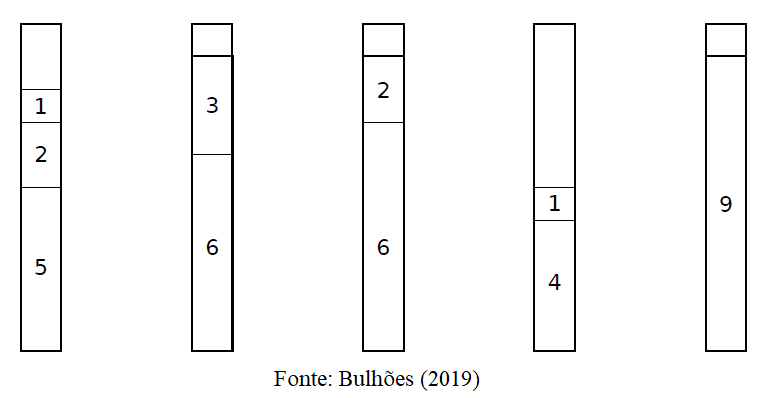
\includegraphics[scale=0.9]{imagens/ExemploBPP.png}
%    \caption{Exemplo de solução para o BPP.}
%    \label{fig:BPP_example}
%\end{figure}

% cores
\definecolor{Orange}{HTML}{ffd6a5}
\definecolor{Red}{HTML}{ffadad}
\definecolor{Yellow}{HTML}{fdffb6}
\definecolor{Blue}{HTML}{9bf6ff}
\definecolor{Green}{HTML}{caffbf}
\definecolor{Dark_blue}{HTML}{a0c4ff}
\definecolor{Violet}{HTML}{bdb2ff}

\pgfdeclarelayer{nodelayer}
\pgfsetlayers{nodelayer}

\begin{figure}[htpb!]
    \centering
    \scalebox{1.0}{
        \begin{tikzpicture}
        	\begin{pgfonlayer}{nodelayer}
        	    % bin 1
        		\node [rectangle, draw = black, minimum height = 2cm, outer sep = 0pt, minimum width = 1cm, thick] (45) at (-4, 4) {};
        		\node [rectangle, draw = black, minimum height = 1cm, outer sep = 0pt, fill=Orange, minimum width = 1cm, thick] (40) at (-4, 2.5) {$w_8$};
        		\node [rectangle, draw = black, minimum height = 2cm, outer sep = 0pt, fill=Blue, minimum width = 1cm, thick] (41) at (-4, 1) {$w_6$};
        		\node [rectangle, draw = black, minimum height = 5cm, outer sep = 0pt, fill=Red, minimum width = 1cm, thick] (42) at (-4, -2.5) {$w_3$};
        		% bin 2
        		\node [rectangle, draw = black, minimum height = 1cm, outer sep = 0pt, minimum width = 1cm, thick] (46) at (-2, 4.5) {};
        		\node [rectangle, draw = black, minimum height = 3cm, outer sep = 0pt, fill=Yellow, minimum width = 1cm, thick] (44) at (-2, 2.5) {$w_4$};
        		\node [rectangle, draw = black, minimum height = 6cm, outer sep = 0pt, fill=Green, minimum width = 1cm, thick] (43) at (-2, -2) {$w_5$};
        		% bin 3
        		\node [rectangle, draw = black, minimum height = 2cm, outer sep = 0pt, minimum width = 1cm, thick] (47) at (0, 4) {};
        		\node [rectangle, draw = black, minimum height = 2cm, outer sep = 0pt, fill=Blue, minimum width = 1cm, thick] (48) at (0, 2) {$w_2$};
        		\node [rectangle, draw = black, minimum height = 6cm, outer sep = 0pt, fill=Green, minimum width = 1cm, thick] (49) at (0, -2) {$w_7$};
        		% bin 4
        		\node[rectangle, draw = black, minimum height = 1cm, outer sep = 0pt, minimum width = 1cm, thick] (54) at (2, 4.5) {};
        		\node [rectangle, draw = black, minimum height = 9cm, outer sep = 0pt, fill=Dark_blue, minimum width = 1cm, thick] (50) at (2, -0.5) {$w_{10}$};
        		% bin 5
        		\node [rectangle, draw = black, minimum height = 5cm, outer sep = 0pt, minimum width = 1cm, thick] (53) at (4, 2.5) {};
        		\node [rectangle, draw = black, minimum height = 1cm, outer sep = 0pt, fill=Orange, minimum width = 1cm, thick] (51) at (4, -0.5) {$w_1$};
        		\node [rectangle, draw = black, minimum height = 4cm, outer sep = 0pt, fill=Violet, minimum width = 1cm, thick] (52) at (4, -3) {$w_9$};
        	\end{pgfonlayer}
        \end{tikzpicture}
    }
    \caption{Exemplo de solução para o BPP.}
    \label{fig:BPP_example}
\end{figure}


\section{Fundamentação teórica do algoritmo} \label{sec:algoritmo}
    \subsection{Simplex Revisado}
        O Simplex Revisado pode ser entendido como uma versão menos computacionalmente custosa do tradicional algoritmo Simplex desenvolvido por George Dantzig(REF). Utilizando-se de métodos eficientes na resolução de sistemas lineares e na atualização da matriz Básica inversa, é possível reduzir a complexidade de $O(m^{3} + mn)$ para $O(m^{2} + mn)$, sendo $m$ e $n$ os números de restrições e de variáveis, respectivamente. Um breve resumo do algoritmo pode ser encontrada a seguir (ref da Tabela do SR):
        % Utilizando-se apenas operações de multiplicação entre matriz e vetor na resolução de sistemas lineares e obtendo um método eficiente para atualizar a matriz Básica inversa
        
        %A seguir, as definições necessárias:
        
% NOTE(victor): nao sei se essa eh a melhor maneira de definir esses itens ae. tlvz seja necessário rever a necessidade dessas definicoes posteriormente 
        %\begin{itemize}
        %   \item $B$: matriz Básica;
        %    \item $\overline{B}$: matriz Básica atualizada;
        %    \item $A$: matriz de coeficientes;
        %    \item $b$: mão-direita;
        %    \item $x_B$: variáveis primais básicas;
        %    \item $\pi$: variáveis duais;
        %    \item $d$: direção;
        %    \item $t$: escalar positivo associado a $d$;
        %\end{itemize}
        
        %O algoritmo pode ser resumido da seguinte maneira:
        
        \begin{table}[htpb!]
        \centering
        \begin{tabular}{|p{0.015\textwidth}p{.85\textwidth}p{0.015\textwidth}|}
        \hline
         &         &  \\
         & \begin{description}
            \item[1a etapa/passo:] Define-se uma solução básica inicial $x_B$, uma matriz básica $B$ e calcula-se $B^{-1}$.
            
            \item[2o passo:] São calculados os custos reduzidos $\overline{c}$ das variáveis não básicas, por meio de $ \overline{c}_j = c_j - \pi A_j $, onde $ \pi = c_B B^{-1}$ , de maneira a selecionar qual irá fazer parte da base -- no caso, a variável que possuir o menor custo reduzido. A otimalidade é alcançada se nenhuma das possuir custo reduzido negativo. Essa etapa é conhecida como \textit{pricing}.
            
            \item[3o passo:] O vetor $ u $ que a determina direção de uma próxima solução básica $x_{\overline{B}}$ é dado por $ u = B^{-1} A_j $, sendo $A_j$ a coluna referente à variável selecionada no 2o passo/etapa.
            
            \item[4o passo:] Determina-se o escalar positivo $ t $ associado a $ u $ e à variável $x_{B(\ell)}$ que sairá da base.
            \end{description}
            
                $$\begin{aligned}
                    && t = \text{min}_{\{i = 1...m | u_i > 0\}}& \frac{x_{B(i)}}{u_i} &
                \end{aligned}$$
                
            \begin{description}
            \item[5o passo:] Seja $\overline{B} $ a matriz básica da próxima solução. Obtém-se uma nova solução básica $ x_{\overline{B}}$, onde $ x_{\overline{B}(\ell)} = t $ e $        x_{\overline{B}(i)} = x_{B(i)} - t u_i, \ \ i \neq \ell $.
                %$$ x_{\overline{B}(i)} = x_{B(i)} - t u_i, \ \ i \neq \ell $$
                %$$ x_{\overline{B}(\ell)} = t $$
            
            \item[6o passo:] $\overline{B}^{-1} $ é calculada de maneira eficiente. Essa etapa consiste na aplicação de um certo conjunto de operações elementares de linha à/na matriz $ B^{-1} $ de mareira que $\overline{B}^{-1} $ seja obtida após o processo. Tal conjunto é o mesmo necessário para que $ e_{\ell} $ seja obtido a partir de $ u $, sendo $ e_{\ell} $ um vetor unitário onde o $\ell$-ésimo elemento é igual a 1 e os demais iguais a 0. Retornasse ao 2o passo.
            
            \end{description} &  \\
         &    &  \\
 
        \hline
        \end{tabular}
        \caption{Descrição Simplex Revisado.}
        % citar o bertsimas ae
        \end{table}
        
        %Realizar o 6o passo requer aplicar um certo conjunto de operações elementares de linha na matriz $ B^{-1} $ de mareira que $\overline{B}^{-1} $ seja obtida após o processo. Tal conjunto é o mesmo necessário para que $ e_{\ell} $ seja obtido a partir de $ u $, sendo $ e_{\ell} $ um vetor unitário onde o $\ell$-ésimo elemento é igual a 1 e os demais iguais a 0.

            % 1) Solução básica inicial e cálculo prévio de B^-1
            % 2) Pricing
                % Calcular custos reduzidos e selecionar  variável para entrar na base
            % 3) Definir direção d
            % 4) Teste da razão mínima (definir escalar t)
            % 5) Atualizar Base e solução básica
            % 6) Calcular \overline{B^-1} de maneira eficiente
            
    %\subsection{Decomposição \textit{Dantzig-Wolfe}}
    %\subsection{Geração de Colunas}

\section{Implementando a Geração de Colunas} \label{sec:implementandoGC}

\section{Implementando a estrutura do \textit{branching}} \label{sec:implementandoBranching}

\section{Conjunto de instâncias} \label{sec:instancias}

Instâncias, e suas soluções ótimas, para o \textit{BPP} podem ser encontradas em \cite{bpplib}\footnote{Link direto: \url{http://or.dei.unibo.it/library/bpplib}} e possuem o seguinte formato:

\begin{table}[htpb!]
\centering
\begin{tabular}{|llll|}
\hline
 &         &                          &  \\
 & $ n $   &                          &  \\
 & $ Q $   &                          &  \\
 & $ w_i $ & $ \ \forall  i  \in  I $ &  \\
 &         &                          &  \\ \hline
\end{tabular}
\caption{Instância do \textit{BPP}.}
\end{table}

Devido a fácil compreensão das instâncias, a leitura pode ser realizada de maneira simples.

%\appendix

\chapter{Repositório}
O repositório se encontra neste \textit{link}: \url{https://github.com/carlosvinicius01/kit-opt}


\nocite{*}
\bibliographystyle{plain}
\bibliography{references}

\end{document}
